% DBMS project report: Smart Hospital Management System.
% Build (from docs/report):  node gen/gen-er.js && node gen/gen-tables.js && tectonic -X compile main.tex
% The structure follows the course template (DBMS_Project.pdf): title page, contents, general instructions,
% chapters 1-11, references, appendices A-D and the evaluation scheme.
\documentclass[10pt,a4paper,oneside]{report}
\usepackage[a4paper,left=2cm,right=2cm,top=1.9cm,bottom=1.9cm,footskip=0.9cm]{geometry}
\usepackage[T1]{fontenc}
\usepackage{lmodern}
\usepackage[english]{babel}
\usepackage{microtype}
\usepackage{amsmath,amssymb}
\usepackage{graphicx}
\usepackage{xcolor}
\usepackage{booktabs,longtable,tabularx,array,multirow}
\usepackage{enumitem}
\usepackage{caption}
\usepackage{float}
\usepackage[normalem]{ulem}
\usepackage{listings}
\usepackage{titlesec}
\usepackage{tikz}
\usetikzlibrary{shapes.geometric,positioning,calc,arrows.meta,fit}
\usepackage{etoolbox}
% chapters follow on from the previous one (after a gap) instead of always starting a new page; this keeps the
% report within its page budget. Chapter 1 and the appendices start on a new page explicitly.
\makeatletter\patchcmd{\chapter}{\if@openright\cleardoublepage\else\clearpage\fi}{\par\addvspace{16pt}}{}{\PackageWarning{report}{chapter patch failed}}\makeatother
\usepackage[hidelinks]{hyperref}
\usepackage{xurl}
\usepackage{adjustbox}
\newcolumntype{R}[1]{>{\raggedright\arraybackslash}p{#1}}
\newcolumntype{Y}{>{\raggedright\arraybackslash}X}

\graphicspath{{figures/}}
% Chen-notation styles for the ER diagrams (figures/er/*.tex).
\tikzset{
  ent/.style={draw, line width=0.6pt, minimum width=2.25cm, minimum height=0.62cm, inner sep=2pt, font=\sffamily\scriptsize\bfseries, fill=white},
  weakent/.style={ent, double, double distance=1.3pt},
  refent/.style={ent, dashed, align=center, fill=gray!7, font=\sffamily\scriptsize\bfseries, minimum height=0.66cm, inner sep=1.5pt},
  rel/.style={draw, line width=0.6pt, diamond, aspect=2.6, inner sep=0.9pt, font=\sffamily\tiny\bfseries, fill=white},
  idrel/.style={rel, double, double distance=1.1pt},
  att/.style={draw, ellipse, inner xsep=0.3pt, inner ysep=0.1pt, font=\sffamily\tiny, fill=white, minimum height=0.34cm},
  total/.style={draw, double, double distance=1.3pt, line width=0.45pt},
  partial/.style={draw, line width=0.5pt},
  card/.style={font=\sffamily\tiny\bfseries, fill=white, inner sep=0.6pt},
}
% A one-line key under each module diagram.
\newcommand{\minilegend}{\par\smallskip{\tiny\centering
\tikz[baseline=-0.6ex]\node[ent,minimum width=0.8cm,minimum height=0.3cm]{};~entity\quad
\tikz[baseline=-0.6ex]\node[weakent,minimum width=0.8cm,minimum height=0.3cm]{};~weak entity\quad
\tikz[baseline=-0.6ex]\node[refent,minimum width=0.8cm,minimum height=0.3cm]{};~entity on another page\quad
\tikz[baseline=-0.6ex]\node[rel,minimum width=0.7cm]{};~relationship\quad
\tikz[baseline=-0.6ex]\node[idrel,minimum width=0.7cm]{};~identifying\quad
\tikz[baseline=-0.6ex]\node[att]{\underline{key}};\enspace
\tikz[baseline=-0.6ex]\node[att]{\dashuline{partial key}};\enspace
\tikz[baseline=-0.6ex]\node[att,double,double distance=0.8pt]{multivalued};\enspace
\tikz[baseline=-0.6ex]\node[att,dashed]{derived};\quad
\tikz[baseline=-0.6ex]\draw[total](0,0)--(0.6,0);~total\enspace
\tikz[baseline=-0.6ex]\draw[partial](0,0)--(0.6,0);~partial participation\par}}


% ---- layout: compact chapter heads in the template's "Chapter N / Title" form
\titleformat{\chapter}[display]{\normalfont\bfseries}{\Large\chaptertitlename\ \thechapter}{4pt}{\LARGE}
\titlespacing*{\chapter}{0pt}{0pt}{10pt}
\titleformat{\section}{\normalfont\large\bfseries}{\thesection}{0.6em}{}
\titlespacing*{\section}{0pt}{9pt plus 2pt}{4pt}
\titleformat{\subsection}{\normalfont\normalsize\bfseries}{\thesubsection}{0.6em}{}
\titlespacing*{\subsection}{0pt}{6pt plus 2pt}{2pt}
\setlength{\parskip}{3pt}
\setlength{\parindent}{0pt}
\setlist{nosep, leftmargin=1.3em}
\captionsetup{font=small, labelfont=bf, skip=4pt}
\captionsetup[lstlisting]{font=small, labelfont=bf, skip=2pt}
\renewcommand{\lstlistingname}{Listing}
\setcounter{tocdepth}{1}
\renewcommand{\arraystretch}{1.12}

\lstdefinestyle{sql}{language=SQL, basicstyle=\ttfamily\scriptsize, keywordstyle=\bfseries, columns=fullflexible,
  breaklines=true, breakatwhitespace=false, frame=single, framerule=0.4pt, rulecolor=\color{gray!60},
  xleftmargin=2pt, xrightmargin=2pt, aboveskip=4pt, belowskip=4pt, showstringspaces=false, upquote=true,
  morekeywords={REFERENCES, ENGINE, AUTO_INCREMENT, ENUM, CONSTRAINT, CHECK, IF, SIGNAL, TRIGGER, EACH, ROW, BEGIN, END, GENERATED, ALWAYS, VIRTUAL, LIMIT, ANY, ALL, EXISTS, CURDATE, ROLLBACK, COMMIT}}
\lstset{style=sql}

% ---- macros used by the generated files
\newcommand{\placeholder}[1]{\fbox{\textcolor{red!70!black}{\textit{[#1]}}}}
\newcommand{\fk}[2]{\textit{#1}\textsuperscript{\tiny FK\ifx\relax#2\relax\else$\to$#2\fi}}
\newcommand{\gen}{\textsuperscript{\tiny G}}
\newcommand{\relation}[3]{\noindent\textbf{\texttt{#1}}(#2)\ifx\relax#3\relax\else{} \textsc{uk} #3\fi\par\vspace{1.5pt}}
\newcommand{\tbl}[1]{\texttt{#1}}
% generated table rows are read with TeX's primitive \input, which works between rows of a table
\makeatletter\newcommand{\rows}[1]{\@@input #1 }\makeatother
% one query of section 8.6: SQL on the left, its real output (hospital_db_test) on the right
\newcommand{\query}[4]{\par\noindent\begin{minipage}[t]{0.5\textwidth}\vspace{0pt}
  \captionof{lstlisting}{Query #1 (#2). #3}\lstinputlisting{generated/#4.sql}\end{minipage}\hfill
  \begin{minipage}[t]{0.47\textwidth}\vspace{2pt}\captionof{table}{Output of Query #1}\centering\begin{adjustbox}{max width=\linewidth}\begin{tabular}{@{}c@{}}\input{generated/#4-out.tex}\end{tabular}\end{adjustbox}\end{minipage}\par\medskip}

% long identifiers (table and column names) may break after an underscore; a little extra stretch avoids overfull lines
\makeatletter\let\hms@us\_\renewcommand{\_}{\hms@us\allowbreak}\makeatother
\setlength{\emergencystretch}{2.5em}
\hypersetup{pdftitle={Smart Hospital Management System: DBMS Project Report}, pdfauthor={}}

\begin{document}
\pagenumbering{roman}
% ================= title page
\begin{titlepage}
\centering
\vspace*{2.2cm}
{\Large\bfseries Database Management Systems (DBMS)\par}
\vspace{2cm}
{\huge\bfseries Project Report\par}
\vspace{0.8cm}
{\LARGE Smart Hospital Management System\par}
\vspace{2.2cm}
\begin{tabular}{@{}p{4.3cm}p{8cm}@{}}
\textbf{Student Name(s):} & \placeholder{to be filled in} \\[14pt]
\textbf{Roll Number(s):} & \placeholder{to be filled in} \\[14pt]
\textbf{Branch \& Section:} & \placeholder{to be filled in} \\[14pt]
\textbf{Course Instructor:} & Priyankar \\[14pt]
\textbf{Academic Session:} & 2026-2027 (Monsoon Semester) \\
\end{tabular}
\vfill
{\large Department of Computer Science\\ Indian Institute of Information Technology Bhopal\par}
\vspace{1cm}
\end{titlepage}

% ================= contents
\tableofcontents

% ================= general instructions (from the template, with where this report meets each one)
\chapter*{General Instructions}
\addcontentsline{toc}{chapter}{General Instructions}
The course template sets these instructions. The right-hand column says where this report and its submission meet each one.

\begin{tabularx}{\textwidth}{@{}rYY@{}}
\toprule
& \textbf{Instruction} & \textbf{In this project} \\\midrule
1 & The front end may use any language or framework. & React 18 single-page app with a Node.js/Express API (Chapter 9). \\
2 & MySQL is mandatory for creation, storage and queries. & MySQL 9.7.1 (InnoDB) is the only database; every table, constraint, view, trigger and procedure is in MySQL (Chapters 7, 8). \\
3 & Design the database before the application. & ER model (Chapter 3), mapping (Chapter 4), dependencies and normalization (Chapters 5, 6) precede the implementation chapters; schema changes are versioned migrations. \\
4 & Demonstrate the DBMS concepts of the course. & Keys, constraints, joins, subqueries, views, triggers, transactions and locking (Chapters 7, 8). \\
5 & Include diagrams, dependencies, normalization steps, SQL and results. & All outputs shown are from real runs on the test database. \\
6 & Submit the report, source code and a complete MySQL script. & Appendix A (\texttt{hospital\_db\_full.sql}) and Appendix B (repository). \\
7 & Every member must understand the design. & Chapter 3.4 and Chapter 6 explain every design decision in words. \\
\bottomrule
\end{tabularx}

\cleardoublepage
\pagenumbering{arabic}
\chapter{Introduction}

\section{Project Overview}
The \textbf{Smart Hospital Management System} is a web application that runs the daily work of a hospital
on one MySQL database. It covers the path of a patient from registration to discharge: appointments and
visits, triage vital signs, doctors' notes, laboratory orders and results, prescriptions dispensed from a
batch-tracked pharmacy, medication given on the ward, bed and emergency allocation, admissions, billing and
an audit trail of who did what.

Its users are the hospital's staff, each with a role that decides what they may see and do:
\begin{itemize}
\item \textbf{Receptionist:} registers patients, books appointments, marks arrivals, raises bills.
\item \textbf{Nurse:} works the wards they are assigned to: triage, vital signs, the medication administration record (MAR).
\item \textbf{Doctor:} sees the patients in their care, writes notes, orders tests, prescribes, admits and discharges.
\item \textbf{Laboratory staff:} process lab orders and record results with optional report files.
\item \textbf{Pharmacy staff:} dispense prescriptions and receive or adjust stock by batch.
\item \textbf{Administrator:} manages staff accounts, nurse assignments, and reads the audit log and reports.
\end{itemize}

\section{Problem Statement}
In many hospitals these records live on paper or in separate systems: a register at the front desk, a ward
book, a pharmacy stock ledger and a lab file. This causes problems that a shared database prevents:
\begin{itemize}
\item \textbf{Inconsistent copies:} a patient's details are written several times and drift apart.
\item \textbf{Unsafe concurrent use:} two clerks can allocate the same last ICU bed, or two pharmacists dispense the same stock.
\item \textbf{No integrity checks:} a dose can be recorded for the wrong patient, stock can go negative, a result can be filed without an order.
\item \textbf{No accountability:} it is hard to tell who changed or viewed a record.
\end{itemize}

\section{Objectives}
\begin{enumerate}
\item Design a normalized relational schema (BCNF where sound) for hospital operations, from an ER model.
\item Enforce the hospital's rules in the database itself: keys, foreign keys, CHECK constraints, triggers and transactions.
\item Keep concurrent operations correct: bed allocation, dispensing and status changes use row locks in a fixed order.
\item Give each role a web front end that reads and writes the database only through a restricted MySQL account.
\item Record every data change and refused access in an append-only audit log.
\item Verify all of this with automated tests that run against a separate test database.
\end{enumerate}

\section{Scope of the Project}
\textbf{Covered:} patient registration (including the 14-digit ABHA number), appointments, the encounter (visit)
lifecycle, vital signs, consultations, surgery requests, laboratory orders and results with attachments,
prescriptions with structured dosing, a batch-level pharmacy with first-expiry-first-out dispensing, the MAR,
wards, beds, admissions and discharges, emergency cases with ambulances and automatic bed and doctor allocation,
billing, staff accounts, nurse ward assignments, doctor schedules and daily statistics, and the audit log.
\textbf{Not covered:} payments through a gateway, insurance claims, live integration with the national ABDM
health-record network, and multi-hospital operation (Section 11.2).

\section{Software and Hardware Requirements}
\begin{tabularx}{\textwidth}{@{}lY@{}}
\toprule
\textbf{Item} & \textbf{Used in this project} \\\midrule
Database & MySQL 9.7.1, InnoDB, isolation level REPEATABLE READ, \texttt{utf8mb4\_0900\_ai\_ci}, strict SQL mode \\
Back end & Node.js 25 with Express 4, \texttt{mysql2} (promise API, connection pool), JSON Web Tokens, bcrypt, Multer (uploads), Socket.IO 4 \\
Front end & React 18, React Router 6, Vite 4, Axios, Socket.IO client \\
Testing & Node's built-in test runner (\texttt{node:test}); Puppeteer for browser tests \\
Tools & Git and GitHub, Visual Studio Code, MySQL command-line client and \texttt{mysqldump}, draw.io, \LaTeX{} \\
Deployment & Docker Compose on an Azure B2als\_v2 virtual machine (2 vCPU, 4 GiB RAM), Caddy for HTTPS \\
Minimum hardware & 2 CPU cores, 4 GB RAM and 2 GB of disk for MySQL, the API and the browser client; any modern browser for users \\
\bottomrule
\end{tabularx}

\chapter{System Requirements and Analysis}

\section{Functional Requirements}
The system must support these operations (the role that performs each is in brackets):
\begin{itemize}
\item \textbf{Patients:} register, search (name, phone, MRN, ABHA), view and edit a patient; record an age when the date of birth is unknown [Receptionist, Administrator].
\item \textbf{Appointments and visits:} book an appointment with a doctor's slot, mark arrival, triage, start and finish the visit, or cancel it [Receptionist, Nurse, Doctor].
\item \textbf{Clinical records:} record vital signs [Nurse]; write consultation notes, order lab tests, prescribe, request surgery [Doctor].
\item \textbf{Laboratory:} move an order to processing, record the result (auto-flagged against reference ranges), attach the report file [Laboratory].
\item \textbf{Pharmacy:} dispense a prescription from non-expired batches, earliest expiry first; receive and adjust stock by batch; low-stock and expiry views [Pharmacy].
\item \textbf{Ward care:} see assigned wards and beds, record each scheduled dose as given, refused or missed [Nurse].
\item \textbf{Beds, admissions and emergencies:} admit to a free bed, discharge, register emergencies and allocate a bed and doctor [Doctor, Receptionist, Administrator].
\item \textbf{Billing:} create bills, add line items, record payments [Receptionist, Administrator].
\item \textbf{Administration:} manage staff accounts and nurse ward assignments; read the audit log; dashboards and reports [Administrator].
\end{itemize}

\section{Business Rules}
Every rule below is enforced by the schema or by the application code, as stated in the last column.

{\small
\begin{longtable}{@{}R{0.5cm}R{8.2cm}R{7.6cm}@{}}
\toprule
& \textbf{Rule} & \textbf{Enforced by} \\\midrule\endhead
1 & Every patient has a unique MRN (the patient id); an ABHA number, when given, is 14 digits and unique. & PK \tbl{patients.patient\_id}; UNIQUE \tbl{uq\_patients\_abha}; CHECK \tbl{chk\_patients\_abha\_format} \\
2 & A date of birth cannot be in the future. & API validation (\tbl{POST/PUT /api/patients}, 400) \\
3 & A doctor cannot be booked twice for the same date and time. & UNIQUE (\tbl{doctor\_id, appointment\_date, appointment\_time}) \\
4 & A visit moves only ARRIVED $\to$ (TRIAGED) $\to$ IN\_PROGRESS $\to$ FINISHED; it can be CANCELLED before it starts or marked ENTERED\_IN\_ERROR before it finishes; its appointment's status follows it. & State machine in \tbl{utils/encounters.js}, in one transaction with the appointment row locked \\
5 & A patient has at most one ACTIVE admission, and a bed holds at most one. & Locking reads (\tbl{SELECT \dots{} FOR UPDATE}) in the admission and emergency services; triggers mark the bed OCCUPIED / AVAILABLE \\
6 & A doctor's workload counts their ACTIVE admissions and never exceeds their maximum. & Trigger \tbl{after\_admission\_insert} / \tbl{after\_admission\_discharge}; CHECK \tbl{doctors\_chk\_1} \\
7 & Stock can never become negative. & CHECK on \tbl{medicines} and \tbl{medicine\_batches}; trigger \tbl{before\_medicine\_stock\_update} \\
8 & A medicine's stock is the sum of its batches; dispensing takes non-expired batches, earliest expiry first. & Same-transaction updates with rows locked in medicine-id order (\tbl{dispenseService}) \\
9 & A prescription item is dispensed at most once, and a dispense time implies it was dispensed. & Guard \tbl{AND dispensed = FALSE} (409 on a second dispense); CHECK \tbl{chk\_prescription\_items\_dispensed} \\
10 & A record filed under a visit, admission, note or batch belongs to the same patient (or medicine). & Composite foreign keys \tbl{fk\_ctx\_*} (15) and API checks (400) \\
11 & A bill's paid amount never exceeds its total; a line's total is quantity $\times$ unit price. & CHECK \tbl{bills\_chk\_2}; generated column \tbl{bill\_items.total\_price} \\
12 & An order has at most one result. & UNIQUE \tbl{lab\_results.order\_id} \\
13 & A dose recorded as given has a time; a scheduled dose exists once per order and slot. & CHECK \tbl{chk\_mar\_given}; UNIQUE (\tbl{prescription\_item\_id, scheduled\_at\_utc}) \\
14 & Vital signs are within physiological ranges and belong to a visit or an admission. & Eleven CHECKs \tbl{chk\_vitals\_*} \\
15 & Discharge is not before admission; a visit does not end before it starts. & CHECK \tbl{admissions\_chk\_1}, \tbl{chk\_encounters\_times} \\
16 & A user account has at most one doctor profile. & UNIQUE \tbl{uq\_doctors\_user\_id} \\
17 & Each action is limited to the roles that may perform it; a doctor sees only patients in their care. & \tbl{authorize(...)} middleware on every route; care-set check in \tbl{utils/patientAccess.js} \\
18 & The audit log can only grow. & Triggers \tbl{audit\_logs\_no\_update} and \tbl{audit\_logs\_no\_delete} \\
\bottomrule
\end{longtable}}

\chapter{Entity--Relationship (ER) Modeling}

\section{Identification of Entities}
The model has 30 entity types in six modules. Each becomes one table (Chapter 4); the two M:N and
ternary relationships with attributes become the other two tables, and \tbl{schema\_migrations} records applied
schema versions and is not part of the domain. Table~\ref{tab:entities} lists every entity with its identifier;
the diagrams show each entity's principal attributes, and Section~4.3 lists all 342 columns.
Four entities are \textbf{weak} (Section~3.4).

{\scriptsize
\begin{longtable}{@{}llllp{4.2cm}@{}}
\caption{Entities, their module, table and identifier}\label{tab:entities}\\
\toprule
\textbf{Entity} & \textbf{Mod.} & \textbf{Table} & \textbf{Type} & \textbf{Identifier (key / partial key)} \\\midrule\endfirsthead
\toprule\textbf{Entity} & \textbf{Mod.} & \textbf{Table} & \textbf{Type} & \textbf{Identifier} \\\midrule\endhead
\rows{figures/er/entity-table.tex}
\bottomrule
\end{longtable}}

\section{Identification of Relationships}
There are 69 relationship types. 64 are binary 1:N, three are binary 1:1 (\textsc{becomes},
\textsc{yields}, \textsc{is\_doctor}) and two carry attributes: \textsc{filled\_from} is M:N (a prescription line can be filled
from several batches, and a batch fills many lines) and \textsc{occupies} is ternary (bed, admission, patient).
Together they account for every one of the 72 relationship foreign keys of the schema; a script checks this,
and checks each participation and cardinality below against the column's nullability and unique keys.
In Table~\ref{tab:rels} the ratio and participation are given in the order the entities are listed
(T = total, P = partial); $^{\ast}$ marks an identifying relationship.

{\tiny\setlength{\tabcolsep}{2.2pt}
\begin{longtable}{@{}llll|llll@{}}
\caption{Relationships, cardinality ratios and participation}\label{tab:rels}\\
\toprule
\textbf{Relationship} & \textbf{Entities} & \textbf{Ratio} & \textbf{Part.} & \textbf{Relationship} & \textbf{Entities} & \textbf{Ratio} & \textbf{Part.} \\\midrule\endfirsthead
\toprule\textbf{Relationship} & \textbf{Entities} & \textbf{Ratio} & \textbf{Part.} & \textbf{Relationship} & \textbf{Entities} & \textbf{Ratio} & \textbf{Part.} \\\midrule\endhead
\rows{figures/er/rel-table.tex}
\bottomrule
\end{longtable}}

\section{ER Diagram}
The diagrams use Chen notation (legend in Figure~\ref{fig:legend}). Figure~\ref{fig:overview} shows the six
modules and the 39 relationships between modules. Figures~\ref{fig:m1a}--\ref{fig:m6b} show the modules one
page at a time; three modules take two pages. An entity drawn in another module appears as a dashed reference box
(``see Module $n$''), and every relationship between two modules is drawn in both, with the same name and cardinality.

\begin{figure}[p]
\centering
% Full legend of the Chen notation used in Figures 3.2 to 3.11.
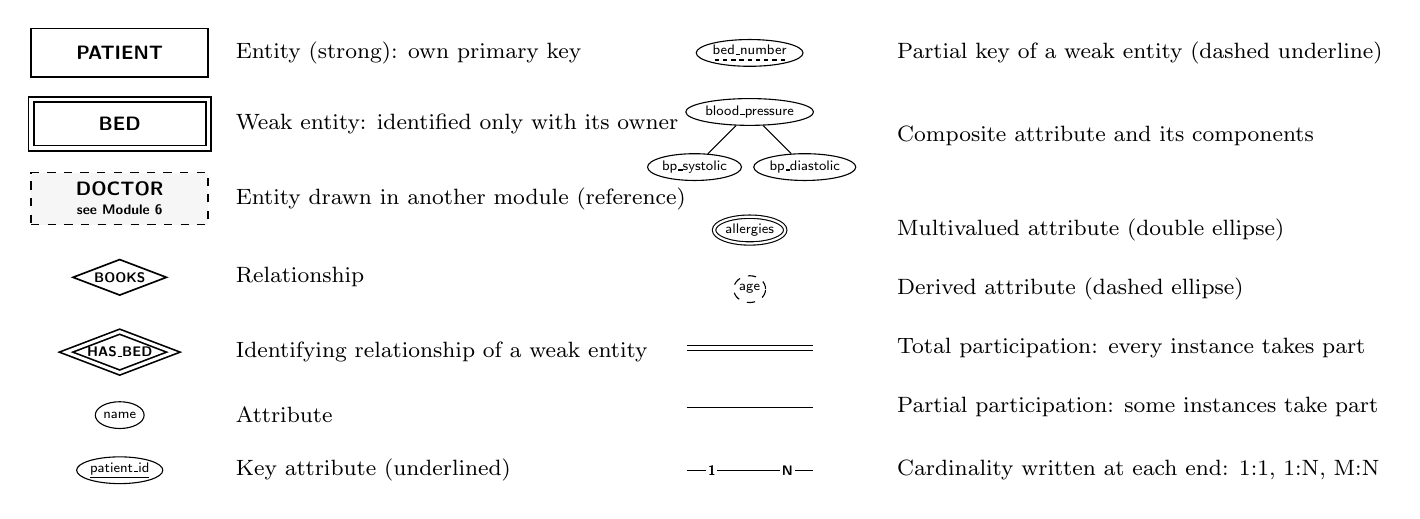
\begin{tikzpicture}[x=1cm,y=1cm, every node/.append style={}]
  \def\row#1#2#3{\node[anchor=west, font=\footnotesize] at (#1+2.35, #2) {#3};}
  % column 1
  \node[ent] at (1,0) {PATIENT};                         \row{0}{0}{Entity (strong): own primary key}
  \node[weakent] at (1,-0.9) {BED};                      \row{0}{-0.9}{Weak entity: identified only with its owner}
  \node[refent] at (1,-1.85) {DOCTOR\\[-1pt]{\tiny see Module 6}}; \row{0}{-1.85}{Entity drawn in another module (reference)}
  \node[rel] at (1,-2.85) {BOOKS};                       \row{0}{-2.85}{Relationship}
  \node[idrel] at (1,-3.8) {HAS\_BED};                   \row{0}{-3.8}{Identifying relationship of a weak entity}
  \node[att] at (1,-4.6) {name};                         \row{0}{-4.6}{Attribute}
  \node[att] at (1,-5.3) {\underline{patient\_id}};      \row{0}{-5.3}{Key attribute (underlined)}
  % column 2
  \node[att] at (9.0,0) {\dashuline{bed\_number}};       \row{8.4}{0}{Partial key of a weak entity (dashed underline)}
  \node[att] (c) at (9.0,-0.75) {blood\_pressure};
  \node[att] (c1) at (8.3,-1.45) {bp\_systolic}; \node[att] (c2) at (9.7,-1.45) {bp\_diastolic}; \draw (c)--(c1) (c)--(c2);
                                                          \row{8.4}{-1.05}{Composite attribute and its components}
  \node[att,double,double distance=0.8pt] at (9.0,-2.25) {allergies}; \row{8.4}{-2.25}{Multivalued attribute (double ellipse)}
  \node[att,dashed] at (9.0,-3.0) {age};                 \row{8.4}{-3.0}{Derived attribute (dashed ellipse)}
  \draw[total] (8.2,-3.75) -- (9.8,-3.75);              \row{8.4}{-3.75}{Total participation: every instance takes part}
  \draw[partial] (8.2,-4.5) -- (9.8,-4.5);              \row{8.4}{-4.5}{Partial participation: some instances take part}
  \draw[partial] (8.2,-5.3) -- node[card,pos=0.2]{1} node[card,pos=0.8]{N} (9.8,-5.3); \row{8.4}{-5.3}{Cardinality written at each end: 1:1, 1:N, M:N}
\end{tikzpicture}

\caption{Legend of the Chen notation used in all ER diagrams}\label{fig:legend}
\vspace{6mm}
% Overview: the six modules and every relationship between two modules (labels: figures/er/overview-labels.tex,
% generated from gen/er-model.js). Module 2 sits inside the triangle 1-5-6 and Module 4 outside it, so no
% two module links cross.
\newcommand{\ovlAB}{PRESCRIBED 1:N\\RX\_IN 1:N\\RX\_FROM 1:N\\SURGERY\_OF 1:N\\SURGERY\_IN 1:N}
\newcommand{\ovlAD}{TESTED 1:N\\LAB\_IN 1:N\\LAB\_FROM 1:N}
\newcommand{\ovlAE}{STAY\_VISIT 1:N\\TAKEN\_ON 1:N\\STAY\_NOTE 1:N\\ADMITTED 1:N\\OCCUPIES N:M:1\\ARRIVES 1:N\\BILLED 1:N}
\newcommand{\ovlAF}{ATTENDS 1:N\\CONDUCTS 1:N\\OPENS 1:N\\RECORDS 1:N\\WRITES 1:N}
\newcommand{\ovlBC}{OF\_DRUG 1:N\\FILLED\_FROM M:N}
\newcommand{\ovlBE}{STAY\_RX 1:N\\STAY\_DOSE 1:N}
\newcommand{\ovlBF}{PRESCRIBES 1:N\\GIVEN\_BY 1:N\\REQUESTS 1:N}
\newcommand{\ovlCF}{RECEIVES 1:N\\PERFORMS 1:N}
\newcommand{\ovlDE}{STAY\_LAB 1:N}
\newcommand{\ovlDF}{OFFERS 1:N\\ORDERS 1:N\\ANALYSES 1:N\\UPLOADS 1:N}
\newcommand{\ovlEF}{IN\_DEPT 1:N\\ADMITS 1:N\\ADMITTED\_TO 1:N\\ASSIGNED 1:N\\COVERS 1:N}
\newcommand{\ovcount}{39}

\newcommand{\ovmA}{\textbf{Module 1: Patients and visits}\\[1pt]{\tiny PATIENT, APPOINTMENT, ENCOUNTER, VITAL\textunderscore{}SIGN, CONSULTATION}}
\newcommand{\ovmB}{\textbf{Module 2: Clinical orders}\\[1pt]{\tiny PRESCRIPTION, PRESCRIPTION\textunderscore{}ITEM, MED\textunderscore{}ADMINISTRATION, SURGERY\textunderscore{}REQUEST}}
\newcommand{\ovmC}{\textbf{Module 3: Pharmacy}\\[1pt]{\tiny MEDICINE, MEDICINE\textunderscore{}BATCH, STOCK\textunderscore{}MOVEMENT}}
\newcommand{\ovmD}{\textbf{Module 4: Laboratory}\\[1pt]{\tiny LAB\textunderscore{}TEST, LAB\textunderscore{}ORDER, LAB\textunderscore{}RESULT, LAB\textunderscore{}ATTACHMENT}}
\newcommand{\ovmE}{\textbf{Module 5: Beds and admissions}\\[1pt]{\tiny WARD, BED, ADMISSION, EMERGENCY\textunderscore{}CASE, AMBULANCE, BILL, BILL\textunderscore{}ITEM}}
\newcommand{\ovmF}{\textbf{Module 6: Staff and audit}\\[1pt]{\tiny USER, DOCTOR, DEPARTMENT, DOCTOR\textunderscore{}SCHEDULE, DAILY\textunderscore{}ANALYTICS, WARD\textunderscore{}ASSIGNMENT, AUDIT\textunderscore{}LOG}}

\begin{tikzpicture}[x=1cm,y=0.78cm,
  mod/.style={draw, line width=0.9pt, rounded corners=3pt, fill=#1, align=center, text width=3.7cm, inner sep=4pt, font=\sffamily\scriptsize, execute at begin node={\hyphenpenalty=10000\exhyphenpenalty=10000}},
  link/.style={line width=0.7pt, gray!70!black},
  lab/.style={fill=white, draw=gray!60, rounded corners=1pt, align=center, font=\sffamily\tiny, inner sep=1.5pt}]
  \node[mod=blue!8]   (M1) at (8.5, 0)     {\ovmA};
  \node[mod=orange!10] (M2) at (8.5, -8.3)  {\ovmB};
  \node[mod=yellow!12] (M3) at (8.3, -12.9) {\ovmC};
  \node[mod=violet!8]  (M4) at (14.4, -4.6) {\ovmD};
  \node[mod=green!9]   (M5) at (14.0, -16.4) {\ovmE};
  \node[mod=gray!12]   (M6) at (3.0, -16.4)  {\ovmF};
  \draw[link] (M1) -- node[lab, pos=0.5] {\ovlAB} (M2);
  \draw[link] (M1) -- node[lab, pos=0.42] {\ovlAF} (M6);
  \draw[link] (M1) -- node[lab, pos=0.47] {\ovlAE} (M5);
  \draw[link] (M1) -- node[lab, pos=0.5] {\ovlAD} (M4);
  \draw[link] (M2) -- node[lab, pos=0.55] {\ovlBE} (M5);
  \draw[link] (M2) -- node[lab, pos=0.5] {\ovlBF} (M6);
  \draw[link] (M2) -- node[lab, pos=0.5] {\ovlBC} (M3);
  \draw[link] (M3) -- node[lab, pos=0.5] {\ovlCF} (M6);
  \draw[link] (M4) -- node[lab, pos=0.45] {\ovlDE} (M5);
  \draw[link] (M5) -- node[lab, pos=0.5] {\ovlEF} (M6);
  \draw[link] (M4.east) -- ++(0.5,0) |- node[lab, pos=0.75] {\ovlDF} ($(M6.south)+(0,-1.2)$) -- (M6.south);
\end{tikzpicture}

\caption{Overview: the six modules and every relationship that crosses between two modules (name and cardinality ratio)}\label{fig:overview}
\end{figure}

\begin{figure}[p]\centering
% Generated by docs/report/gen/gen-er.js: diagram 1a (Module 1)
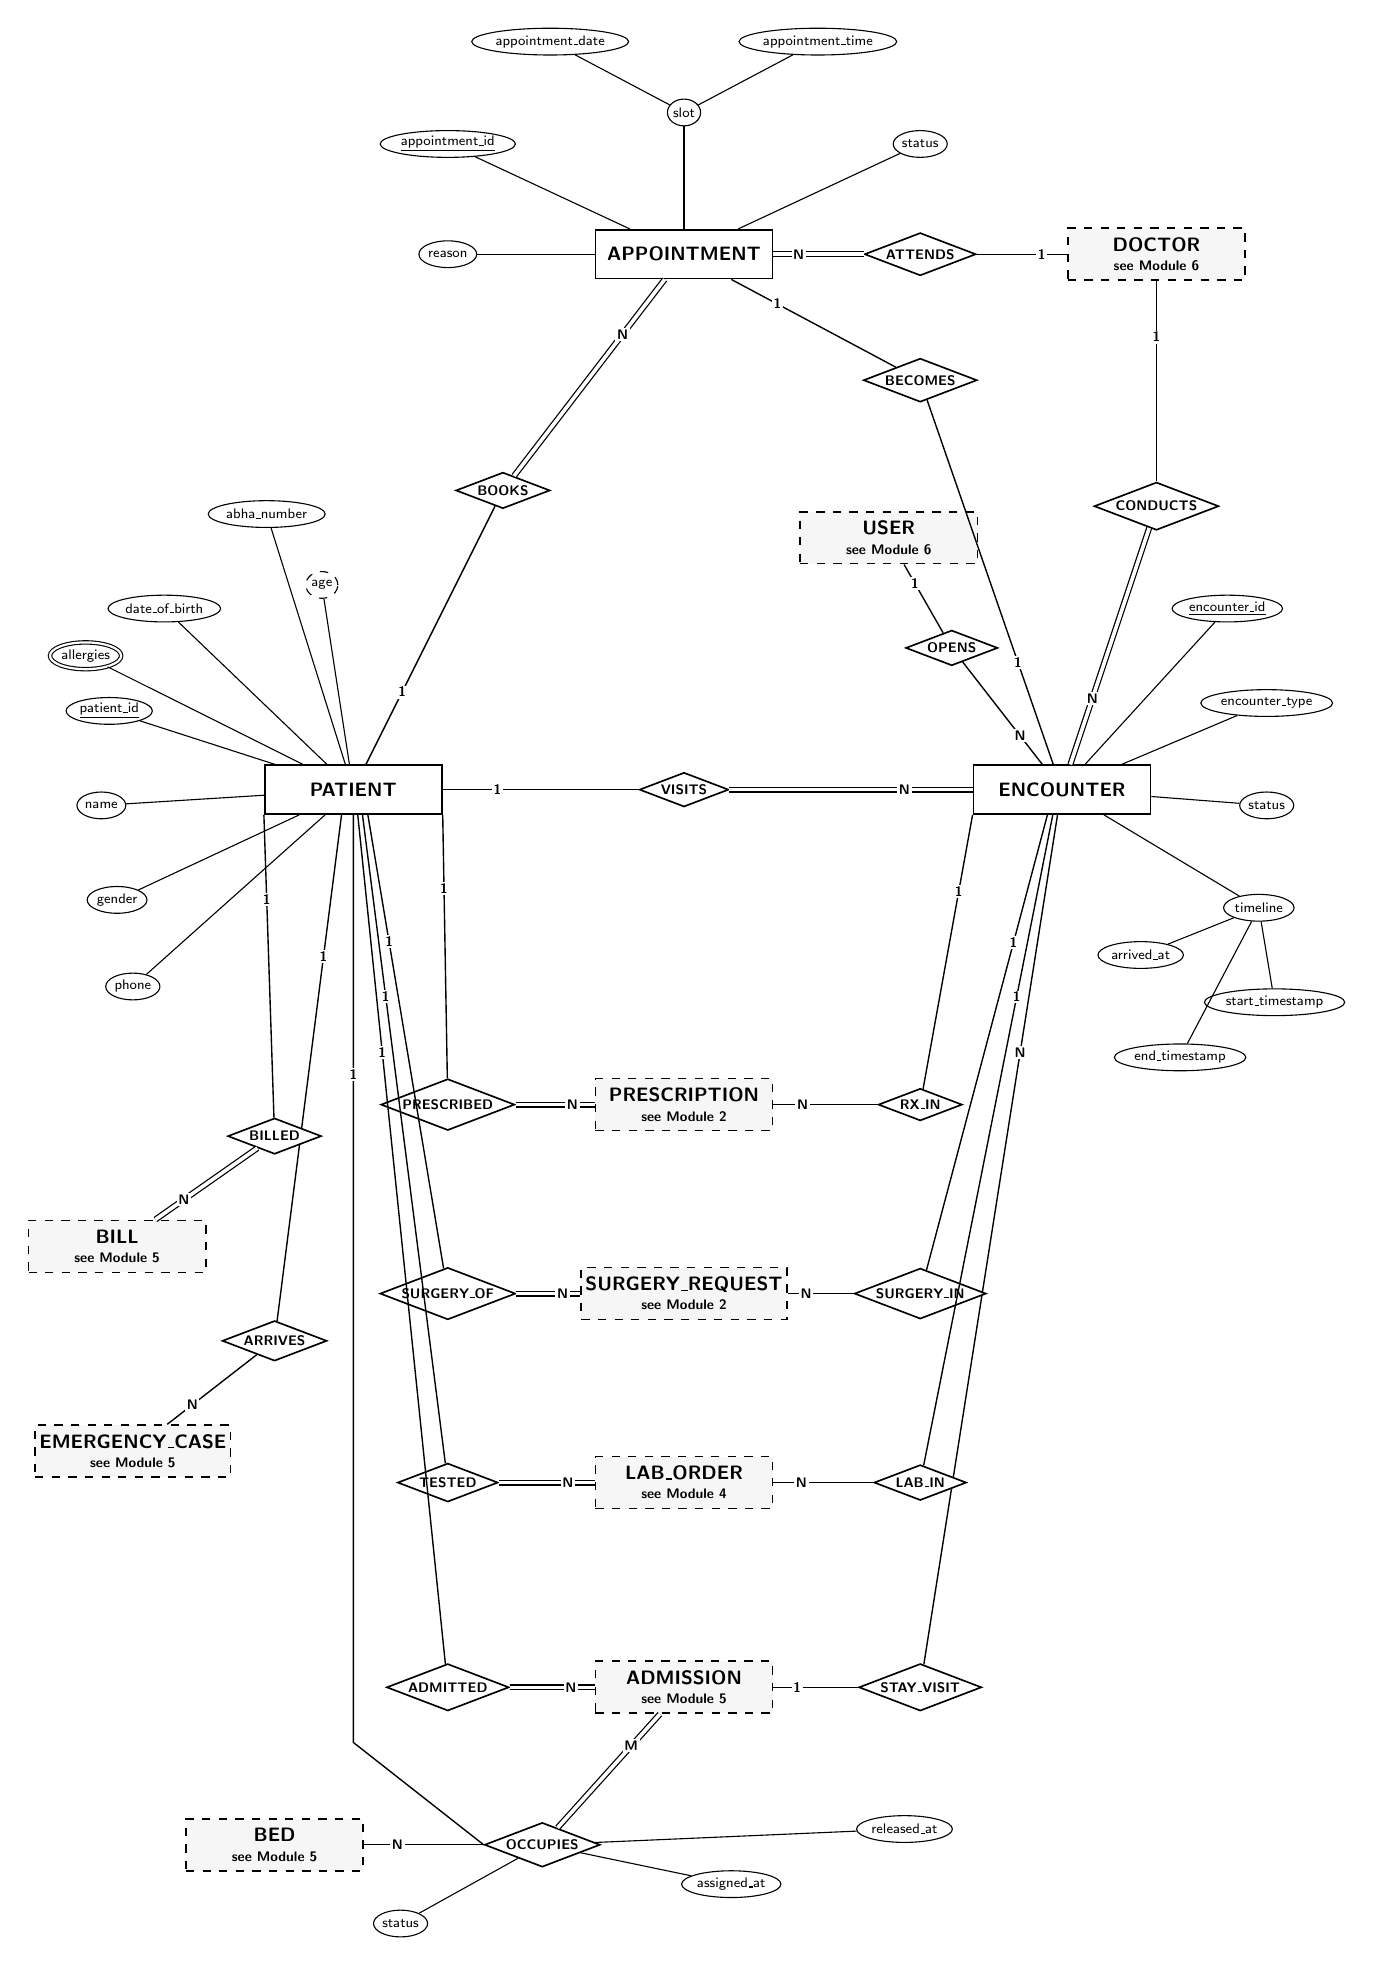
\begin{tikzpicture}[x=1cm,y=1cm]
\node[ent] (PATIENT) at (4.4,-9.2) {PATIENT};
\node[att] (PATIENT-patient_id) at (1.3,-8.2) {\underline{patient\_id}};
\draw (PATIENT-patient_id) -- (PATIENT);
\node[att] (PATIENT-name) at (1.2,-9.4) {name};
\draw (PATIENT-name) -- (PATIENT);
\node[att] (PATIENT-date_of_birth) at (2,-6.9) {date\_of\_birth};
\draw (PATIENT-date_of_birth) -- (PATIENT);
\node[att,dashed] (PATIENT-age) at (4,-6.6) {age};
\draw (PATIENT-age) -- (PATIENT);
\node[att] (PATIENT-gender) at (1.4,-10.6) {gender};
\draw (PATIENT-gender) -- (PATIENT);
\node[att,double,double distance=0.8pt] (PATIENT-allergies) at (1,-7.5) {allergies};
\draw (PATIENT-allergies) -- (PATIENT);
\node[att] (PATIENT-abha_number) at (3.3,-5.7) {abha\_number};
\draw (PATIENT-abha_number) -- (PATIENT);
\node[att] (PATIENT-phone) at (1.6,-11.7) {phone};
\draw (PATIENT-phone) -- (PATIENT);
\node[ent] (APPOINTMENT) at (8.6,-2.4) {APPOINTMENT};
\node[att] (APPOINTMENT-appointment_id) at (5.6,-1) {\underline{appointment\_id}};
\draw (APPOINTMENT-appointment_id) -- (APPOINTMENT);
\node[att] (APPOINTMENT-slot) at (8.6,-0.6) {slot};
\draw (APPOINTMENT-slot) -- (APPOINTMENT);
\node[att] (APPOINTMENT-slot-appointment_date) at (6.9,0.3) {appointment\_date};
\draw (APPOINTMENT-slot-appointment_date) -- (APPOINTMENT-slot);
\node[att] (APPOINTMENT-slot-appointment_time) at (10.3,0.3) {appointment\_time};
\draw (APPOINTMENT-slot-appointment_time) -- (APPOINTMENT-slot);
\node[att] (APPOINTMENT-status) at (11.6,-1) {status};
\draw (APPOINTMENT-status) -- (APPOINTMENT);
\node[att] (APPOINTMENT-reason) at (5.6,-2.4) {reason};
\draw (APPOINTMENT-reason) -- (APPOINTMENT);
\node[ent] (ENCOUNTER) at (13.4,-9.2) {ENCOUNTER};
\node[att] (ENCOUNTER-encounter_id) at (15.5,-6.9) {\underline{encounter\_id}};
\draw (ENCOUNTER-encounter_id) -- (ENCOUNTER);
\node[att] (ENCOUNTER-encounter_type) at (16,-8.1) {encounter\_type};
\draw (ENCOUNTER-encounter_type) -- (ENCOUNTER);
\node[att] (ENCOUNTER-status) at (16,-9.4) {status};
\draw (ENCOUNTER-status) -- (ENCOUNTER);
\node[att] (ENCOUNTER-timeline) at (15.9,-10.7) {timeline};
\draw (ENCOUNTER-timeline) -- (ENCOUNTER);
\node[att] (ENCOUNTER-timeline-arrived_at) at (14.4,-11.3) {arrived\_at};
\draw (ENCOUNTER-timeline-arrived_at) -- (ENCOUNTER-timeline);
\node[att] (ENCOUNTER-timeline-start_timestamp) at (16.1,-11.9) {start\_timestamp};
\draw (ENCOUNTER-timeline-start_timestamp) -- (ENCOUNTER-timeline);
\node[att] (ENCOUNTER-timeline-end_timestamp) at (14.9,-12.6) {end\_timestamp};
\draw (ENCOUNTER-timeline-end_timestamp) -- (ENCOUNTER-timeline);
\node[refent] (DOCTOR) at (14.6,-2.4) {DOCTOR\\[-1pt]{\tiny see Module 6}};
\node[refent] (USER) at (11.2,-6) {USER\\[-1pt]{\tiny see Module 6}};
\node[refent] (PRESCRIPTION) at (8.6,-13.2) {PRESCRIPTION\\[-1pt]{\tiny see Module 2}};
\node[refent] (SURGERY_REQUEST) at (8.6,-15.6) {SURGERY\_REQUEST\\[-1pt]{\tiny see Module 2}};
\node[refent] (LAB_ORDER) at (8.6,-18) {LAB\_ORDER\\[-1pt]{\tiny see Module 4}};
\node[refent] (ADMISSION) at (8.6,-20.6) {ADMISSION\\[-1pt]{\tiny see Module 5}};
\node[refent] (BILL) at (1.4,-15) {BILL\\[-1pt]{\tiny see Module 5}};
\node[refent] (EMERGENCY_CASE) at (1.6,-17.6) {EMERGENCY\_CASE\\[-1pt]{\tiny see Module 5}};
\node[refent] (BED) at (3.4,-22.6) {BED\\[-1pt]{\tiny see Module 5}};
\node[rel] (BOOKS) at (6.3,-5.4) {BOOKS};
\draw[partial] (BOOKS) -- node[card,pos=0.72] {1} (PATIENT);
\draw[total] (BOOKS) -- node[card,pos=0.72] {N} (APPOINTMENT);
\node[rel] (ATTENDS) at (11.6,-2.4) {ATTENDS};
\draw[partial] (ATTENDS) -- node[card,pos=0.72] {1} (DOCTOR);
\draw[total] (ATTENDS) -- node[card,pos=0.72] {N} (APPOINTMENT);
\node[rel] (VISITS) at (8.6,-9.2) {VISITS};
\draw[partial] (VISITS) -- node[card,pos=0.72] {1} (PATIENT);
\draw[total] (VISITS) -- node[card,pos=0.72] {N} (ENCOUNTER);
\node[rel] (CONDUCTS) at (14.6,-5.6) {CONDUCTS};
\draw[partial] (CONDUCTS) -- node[card,pos=0.72] {1} (DOCTOR);
\draw[total] (CONDUCTS) -- node[card,pos=0.72] {N} (ENCOUNTER);
\node[rel] (BECOMES) at (11.6,-4) {BECOMES};
\draw[partial] (BECOMES) -- node[card,pos=0.72] {1} (APPOINTMENT);
\draw[partial] (BECOMES) -- node[card,pos=0.72] {1} (ENCOUNTER);
\node[rel] (OPENS) at (12,-7.4) {OPENS};
\draw[partial] (OPENS) -- node[card,pos=0.72] {1} (USER);
\draw[partial] (OPENS) -- node[card,pos=0.72] {N} (ENCOUNTER);
\node[rel] (STAY_VISIT) at (11.6,-20.6) {STAY\_VISIT};
\draw[partial] (STAY_VISIT) -- node[card,pos=0.72] {1} (ADMISSION);
\draw[partial] (STAY_VISIT) -- node[card,pos=0.72] {N} (ENCOUNTER.-100);
\node[rel] (PRESCRIBED) at (5.6,-13.2) {PRESCRIBED};
\draw[partial] (PRESCRIBED) -- node[card,pos=0.72] {1} (PATIENT.south east);
\draw[total] (PRESCRIBED) -- node[card,pos=0.72] {N} (PRESCRIPTION);
\node[rel] (RX_IN) at (11.6,-13.2) {RX\_IN};
\draw[partial] (RX_IN) -- node[card,pos=0.72] {1} (ENCOUNTER.south west);
\draw[partial] (RX_IN) -- node[card,pos=0.72] {N} (PRESCRIPTION);
\node[rel] (SURGERY_OF) at (5.6,-15.6) {SURGERY\_OF};
\draw[partial] (SURGERY_OF) -- node[card,pos=0.72] {1} (PATIENT.-60);
\draw[total] (SURGERY_OF) -- node[card,pos=0.72] {N} (SURGERY_REQUEST);
\node[rel] (SURGERY_IN) at (11.6,-15.6) {SURGERY\_IN};
\draw[partial] (SURGERY_IN) -- node[card,pos=0.72] {1} (ENCOUNTER.-120);
\draw[partial] (SURGERY_IN) -- node[card,pos=0.72] {N} (SURGERY_REQUEST);
\node[rel] (TESTED) at (5.6,-18) {TESTED};
\draw[partial] (TESTED) -- node[card,pos=0.72] {1} (PATIENT.-70);
\draw[total] (TESTED) -- node[card,pos=0.72] {N} (LAB_ORDER);
\node[rel] (LAB_IN) at (11.6,-18) {LAB\_IN};
\draw[partial] (LAB_IN) -- node[card,pos=0.72] {1} (ENCOUNTER.-110);
\draw[partial] (LAB_IN) -- node[card,pos=0.72] {N} (LAB_ORDER);
\node[rel] (ADMITTED) at (5.6,-20.6) {ADMITTED};
\draw[partial] (ADMITTED) -- node[card,pos=0.72] {1} (PATIENT.-80);
\draw[total] (ADMITTED) -- node[card,pos=0.72] {N} (ADMISSION);
\node[rel] (OCCUPIES) at (6.8,-22.6) {OCCUPIES};
\draw[partial] (OCCUPIES) -- node[card,pos=0.72] {N} (BED);
\draw[total] (OCCUPIES) -- node[card,pos=0.72] {M} (ADMISSION);
\draw[partial] (OCCUPIES.west) -- (4.4,-21.3) -- node[card,pos=0.72] {1} (PATIENT);
\node[att] (OCCUPIES-assigned_at) at (9.2,-23.1) {assigned\_at};
\draw (OCCUPIES-assigned_at) -- (OCCUPIES);
\node[att] (OCCUPIES-released_at) at (11.4,-22.4) {released\_at};
\draw (OCCUPIES-released_at) -- (OCCUPIES);
\node[att] (OCCUPIES-status) at (5,-23.6) {status};
\draw (OCCUPIES-status) -- (OCCUPIES);
\node[rel] (ARRIVES) at (3.4,-16.2) {ARRIVES};
\draw[partial] (ARRIVES) -- node[card,pos=0.72] {1} (PATIENT.-115);
\draw[partial] (ARRIVES) -- node[card,pos=0.72] {N} (EMERGENCY_CASE);
\node[rel] (BILLED) at (3.4,-13.6) {BILLED};
\draw[partial] (BILLED) -- node[card,pos=0.72] {1} (PATIENT.south west);
\draw[total] (BILLED) -- node[card,pos=0.72] {N} (BILL);
\end{tikzpicture}
\minilegend
\caption{Module 1, Patients and visits (page 1 of 2): patients, appointments and encounters}\label{fig:m1a}
\end{figure}

\begin{figure}[p]\centering
% Generated by docs/report/gen/gen-er.js: diagram 1b (Module 1)
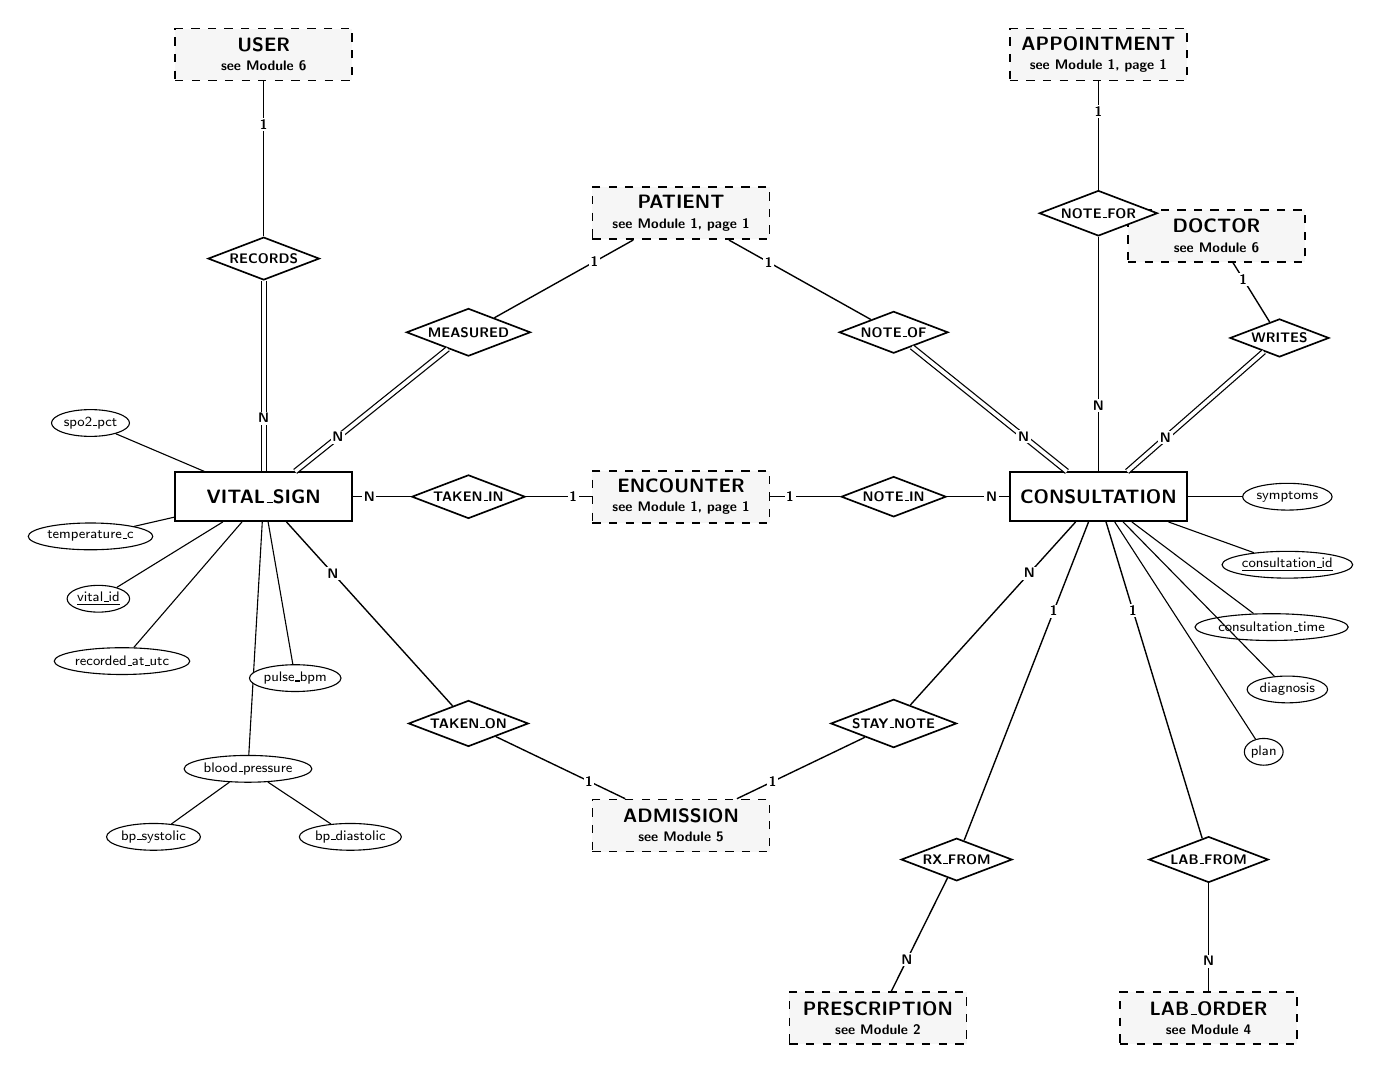
\begin{tikzpicture}[x=1cm,y=0.72cm]
\node[ent] (VITAL_SIGN) at (3.2,-9.2) {VITAL\_SIGN};
\node[att] (VITAL_SIGN-vital_id) at (1.1,-11) {\underline{vital\_id}};
\draw (VITAL_SIGN-vital_id) -- (VITAL_SIGN);
\node[att] (VITAL_SIGN-recorded_at_utc) at (1.4,-12.1) {recorded\_at\_utc};
\draw (VITAL_SIGN-recorded_at_utc) -- (VITAL_SIGN);
\node[att] (VITAL_SIGN-blood_pressure) at (3,-14) {blood\_pressure};
\draw (VITAL_SIGN-blood_pressure) -- (VITAL_SIGN);
\node[att] (VITAL_SIGN-blood_pressure-bp_systolic) at (1.8,-15.2) {bp\_systolic};
\draw (VITAL_SIGN-blood_pressure-bp_systolic) -- (VITAL_SIGN-blood_pressure);
\node[att] (VITAL_SIGN-blood_pressure-bp_diastolic) at (4.3,-15.2) {bp\_diastolic};
\draw (VITAL_SIGN-blood_pressure-bp_diastolic) -- (VITAL_SIGN-blood_pressure);
\node[att] (VITAL_SIGN-pulse_bpm) at (3.6,-12.4) {pulse\_bpm};
\draw (VITAL_SIGN-pulse_bpm) -- (VITAL_SIGN);
\node[att] (VITAL_SIGN-temperature_c) at (1,-9.9) {temperature\_c};
\draw (VITAL_SIGN-temperature_c) -- (VITAL_SIGN);
\node[att] (VITAL_SIGN-spo2_pct) at (1,-7.9) {spo2\_pct};
\draw (VITAL_SIGN-spo2_pct) -- (VITAL_SIGN);
\node[ent] (CONSULTATION) at (13.8,-9.2) {CONSULTATION};
\node[att] (CONSULTATION-consultation_id) at (16.2,-10.4) {\underline{consultation\_id}};
\draw (CONSULTATION-consultation_id) -- (CONSULTATION);
\node[att] (CONSULTATION-consultation_time) at (16,-11.5) {consultation\_time};
\draw (CONSULTATION-consultation_time) -- (CONSULTATION);
\node[att] (CONSULTATION-symptoms) at (16.2,-9.2) {symptoms};
\draw (CONSULTATION-symptoms) -- (CONSULTATION);
\node[att] (CONSULTATION-diagnosis) at (16.2,-12.6) {diagnosis};
\draw (CONSULTATION-diagnosis) -- (CONSULTATION);
\node[att] (CONSULTATION-plan) at (15.9,-13.7) {plan};
\draw (CONSULTATION-plan) -- (CONSULTATION);
\node[refent] (PATIENT) at (8.5,-4.2) {PATIENT\\[-1pt]{\tiny see Module 1, page 1}};
\node[refent] (ENCOUNTER) at (8.5,-9.2) {ENCOUNTER\\[-1pt]{\tiny see Module 1, page 1}};
\node[refent] (APPOINTMENT) at (13.8,-1.4) {APPOINTMENT\\[-1pt]{\tiny see Module 1, page 1}};
\node[refent] (ADMISSION) at (8.5,-15) {ADMISSION\\[-1pt]{\tiny see Module 5}};
\node[refent] (USER) at (3.2,-1.4) {USER\\[-1pt]{\tiny see Module 6}};
\node[refent] (DOCTOR) at (15.299999999999999,-4.6) {DOCTOR\\[-1pt]{\tiny see Module 6}};
\node[refent] (PRESCRIPTION) at (11,-18.4) {PRESCRIPTION\\[-1pt]{\tiny see Module 2}};
\node[refent] (LAB_ORDER) at (15.2,-18.4) {LAB\_ORDER\\[-1pt]{\tiny see Module 4}};
\node[rel] (MEASURED) at (5.8,-6.3) {MEASURED};
\draw[partial] (MEASURED) -- node[card,pos=0.72] {1} (PATIENT);
\draw[total] (MEASURED) -- node[card,pos=0.72] {N} (VITAL_SIGN);
\node[rel] (TAKEN_IN) at (5.8,-9.2) {TAKEN\_IN};
\draw[partial] (TAKEN_IN) -- node[card,pos=0.72] {1} (ENCOUNTER);
\draw[partial] (TAKEN_IN) -- node[card,pos=0.72] {N} (VITAL_SIGN);
\node[rel] (TAKEN_ON) at (5.8,-13.2) {TAKEN\_ON};
\draw[partial] (TAKEN_ON) -- node[card,pos=0.72] {1} (ADMISSION);
\draw[partial] (TAKEN_ON) -- node[card,pos=0.72] {N} (VITAL_SIGN);
\node[rel] (RECORDS) at (3.2,-5) {RECORDS};
\draw[partial] (RECORDS) -- node[card,pos=0.72] {1} (USER);
\draw[total] (RECORDS) -- node[card,pos=0.72] {N} (VITAL_SIGN);
\node[rel] (NOTE_OF) at (11.2,-6.3) {NOTE\_OF};
\draw[partial] (NOTE_OF) -- node[card,pos=0.72] {1} (PATIENT);
\draw[total] (NOTE_OF) -- node[card,pos=0.72] {N} (CONSULTATION);
\node[rel] (WRITES) at (16.1,-6.4) {WRITES};
\draw[partial] (WRITES) -- node[card,pos=0.72] {1} (DOCTOR);
\draw[total] (WRITES) -- node[card,pos=0.72] {N} (CONSULTATION);
\node[rel] (NOTE_IN) at (11.2,-9.2) {NOTE\_IN};
\draw[partial] (NOTE_IN) -- node[card,pos=0.72] {1} (ENCOUNTER);
\draw[partial] (NOTE_IN) -- node[card,pos=0.72] {N} (CONSULTATION);
\node[rel] (NOTE_FOR) at (13.8,-4.2) {NOTE\_FOR};
\draw[partial] (NOTE_FOR) -- node[card,pos=0.72] {1} (APPOINTMENT);
\draw[partial] (NOTE_FOR) -- node[card,pos=0.72] {N} (CONSULTATION);
\node[rel] (STAY_NOTE) at (11.2,-13.2) {STAY\_NOTE};
\draw[partial] (STAY_NOTE) -- node[card,pos=0.72] {1} (ADMISSION);
\draw[partial] (STAY_NOTE) -- node[card,pos=0.72] {N} (CONSULTATION);
\node[rel] (RX_FROM) at (12,-15.6) {RX\_FROM};
\draw[partial] (RX_FROM) -- node[card,pos=0.72] {1} (CONSULTATION);
\draw[partial] (RX_FROM) -- node[card,pos=0.72] {N} (PRESCRIPTION);
\node[rel] (LAB_FROM) at (15.2,-15.6) {LAB\_FROM};
\draw[partial] (LAB_FROM) -- node[card,pos=0.72] {1} (CONSULTATION);
\draw[partial] (LAB_FROM) -- node[card,pos=0.72] {N} (LAB_ORDER);
\end{tikzpicture}
\minilegend
\caption{Module 1, Patients and visits (page 2 of 2): vital signs and consultations}\label{fig:m1b}
\vspace{5mm}
% Generated by docs/report/gen/gen-er.js: diagram 3 (Module 3)
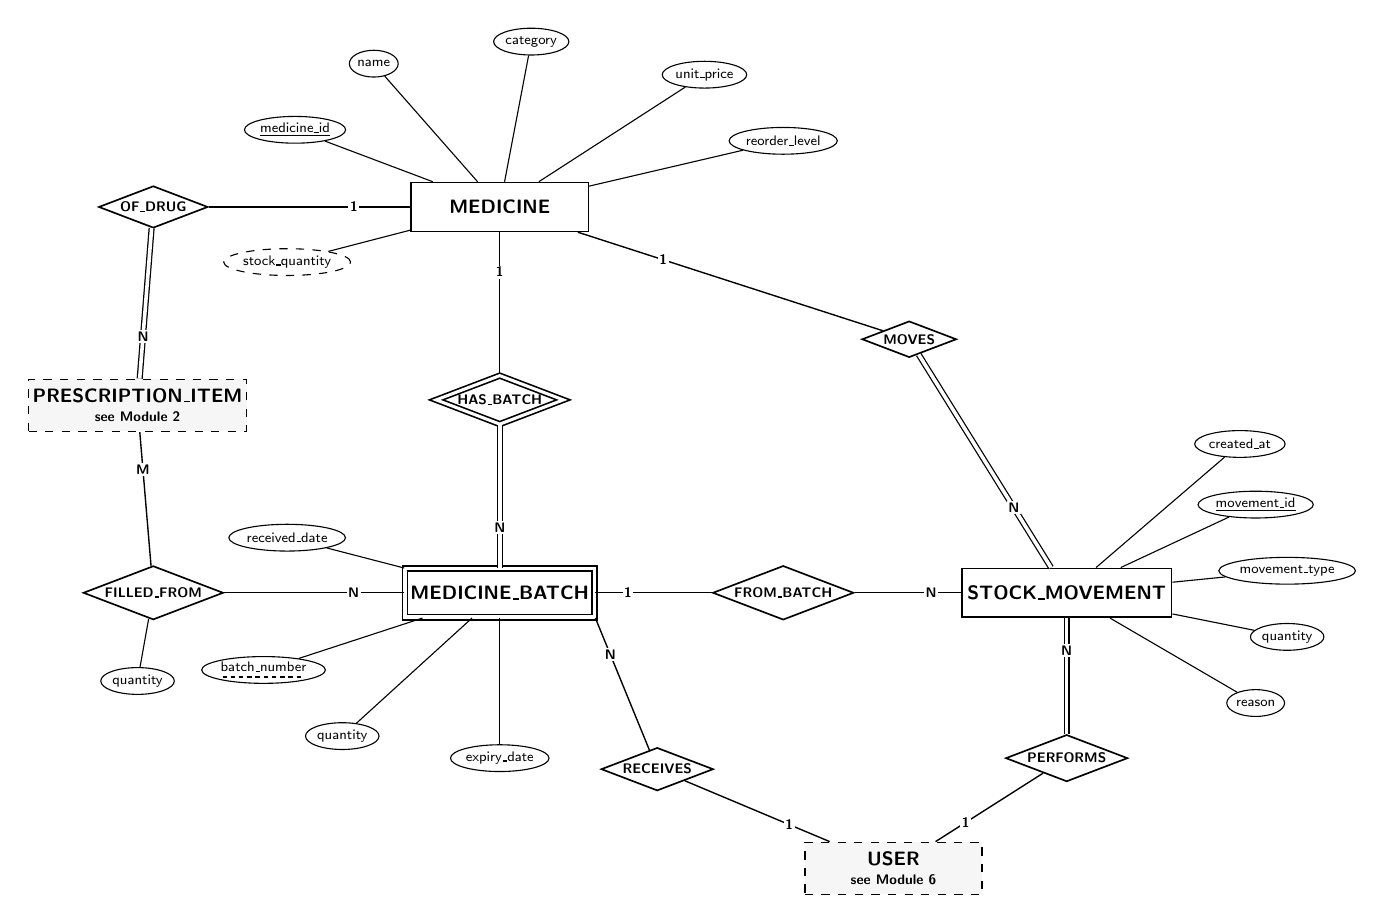
\begin{tikzpicture}[x=1cm,y=0.7cm]
\node[ent] (MEDICINE) at (6,-4) {MEDICINE};
\node[att] (MEDICINE-medicine_id) at (3.4,-2.6) {\underline{medicine\_id}};
\draw (MEDICINE-medicine_id) -- (MEDICINE);
\node[att] (MEDICINE-name) at (4.4,-1.4) {name};
\draw (MEDICINE-name) -- (MEDICINE);
\node[att] (MEDICINE-category) at (6.4,-1) {category};
\draw (MEDICINE-category) -- (MEDICINE);
\node[att] (MEDICINE-unit_price) at (8.6,-1.6) {unit\_price};
\draw (MEDICINE-unit_price) -- (MEDICINE);
\node[att] (MEDICINE-reorder_level) at (9.6,-2.8) {reorder\_level};
\draw (MEDICINE-reorder_level) -- (MEDICINE);
\node[att,dashed] (MEDICINE-stock_quantity) at (3.3,-5) {stock\_quantity};
\draw (MEDICINE-stock_quantity) -- (MEDICINE);
\node[weakent] (MEDICINE_BATCH) at (6,-11) {MEDICINE\_BATCH};
\node[att] (MEDICINE_BATCH-batch_number) at (3,-12.4) {\dashuline{batch\_number}};
\draw (MEDICINE_BATCH-batch_number) -- (MEDICINE_BATCH);
\node[att] (MEDICINE_BATCH-quantity) at (4,-13.6) {quantity};
\draw (MEDICINE_BATCH-quantity) -- (MEDICINE_BATCH);
\node[att] (MEDICINE_BATCH-expiry_date) at (6,-14) {expiry\_date};
\draw (MEDICINE_BATCH-expiry_date) -- (MEDICINE_BATCH);
\node[att] (MEDICINE_BATCH-received_date) at (3.3,-10) {received\_date};
\draw (MEDICINE_BATCH-received_date) -- (MEDICINE_BATCH);
\node[ent] (STOCK_MOVEMENT) at (13.2,-11) {STOCK\_MOVEMENT};
\node[att] (STOCK_MOVEMENT-movement_id) at (15.6,-9.4) {\underline{movement\_id}};
\draw (STOCK_MOVEMENT-movement_id) -- (STOCK_MOVEMENT);
\node[att] (STOCK_MOVEMENT-movement_type) at (16,-10.6) {movement\_type};
\draw (STOCK_MOVEMENT-movement_type) -- (STOCK_MOVEMENT);
\node[att] (STOCK_MOVEMENT-quantity) at (16,-11.8) {quantity};
\draw (STOCK_MOVEMENT-quantity) -- (STOCK_MOVEMENT);
\node[att] (STOCK_MOVEMENT-reason) at (15.6,-13) {reason};
\draw (STOCK_MOVEMENT-reason) -- (STOCK_MOVEMENT);
\node[att] (STOCK_MOVEMENT-created_at) at (15.4,-8.3) {created\_at};
\draw (STOCK_MOVEMENT-created_at) -- (STOCK_MOVEMENT);
\node[refent] (PRESCRIPTION_ITEM) at (1.4,-7.6) {PRESCRIPTION\_ITEM\\[-1pt]{\tiny see Module 2}};
\node[refent] (USER) at (11,-16) {USER\\[-1pt]{\tiny see Module 6}};
\node[rel] (OF_DRUG) at (1.6,-4) {OF\_DRUG};
\draw[partial] (OF_DRUG) -- node[card,pos=0.72] {1} (MEDICINE.west);
\draw[total] (OF_DRUG) -- node[card,pos=0.72] {N} (PRESCRIPTION_ITEM);
\node[rel] (FILLED_FROM) at (1.6,-11) {FILLED\_FROM};
\draw[partial] (FILLED_FROM) -- node[card,pos=0.72] {M} (PRESCRIPTION_ITEM);
\draw[partial] (FILLED_FROM) -- node[card,pos=0.72] {N} (MEDICINE_BATCH.west);
\node[att] (FILLED_FROM-quantity) at (1.4,-12.6) {quantity};
\draw (FILLED_FROM-quantity) -- (FILLED_FROM);
\node[idrel] (HAS_BATCH) at (6,-7.5) {HAS\_BATCH};
\draw[partial] (HAS_BATCH) -- node[card,pos=0.72] {1} (MEDICINE);
\draw[total] (HAS_BATCH) -- node[card,pos=0.72] {N} (MEDICINE_BATCH);
\node[rel] (RECEIVES) at (8,-14.2) {RECEIVES};
\draw[partial] (RECEIVES) -- node[card,pos=0.72] {1} (USER);
\draw[partial] (RECEIVES) -- node[card,pos=0.72] {N} (MEDICINE_BATCH.south east);
\node[rel] (MOVES) at (11.2,-6.4) {MOVES};
\draw[partial] (MOVES) -- node[card,pos=0.72] {1} (MEDICINE);
\draw[total] (MOVES) -- node[card,pos=0.72] {N} (STOCK_MOVEMENT);
\node[rel] (FROM_BATCH) at (9.6,-11) {FROM\_BATCH};
\draw[partial] (FROM_BATCH) -- node[card,pos=0.72] {1} (MEDICINE_BATCH);
\draw[partial] (FROM_BATCH) -- node[card,pos=0.72] {N} (STOCK_MOVEMENT);
\node[rel] (PERFORMS) at (13.2,-14) {PERFORMS};
\draw[partial] (PERFORMS) -- node[card,pos=0.72] {1} (USER);
\draw[total] (PERFORMS) -- node[card,pos=0.72] {N} (STOCK_MOVEMENT);
\end{tikzpicture}
\minilegend
\caption{Module 3, Pharmacy: medicines, batches and stock movements}\label{fig:m3}
\end{figure}

\begin{figure}[p]\centering
% Generated by docs/report/gen/gen-er.js: diagram 2 (Module 2)
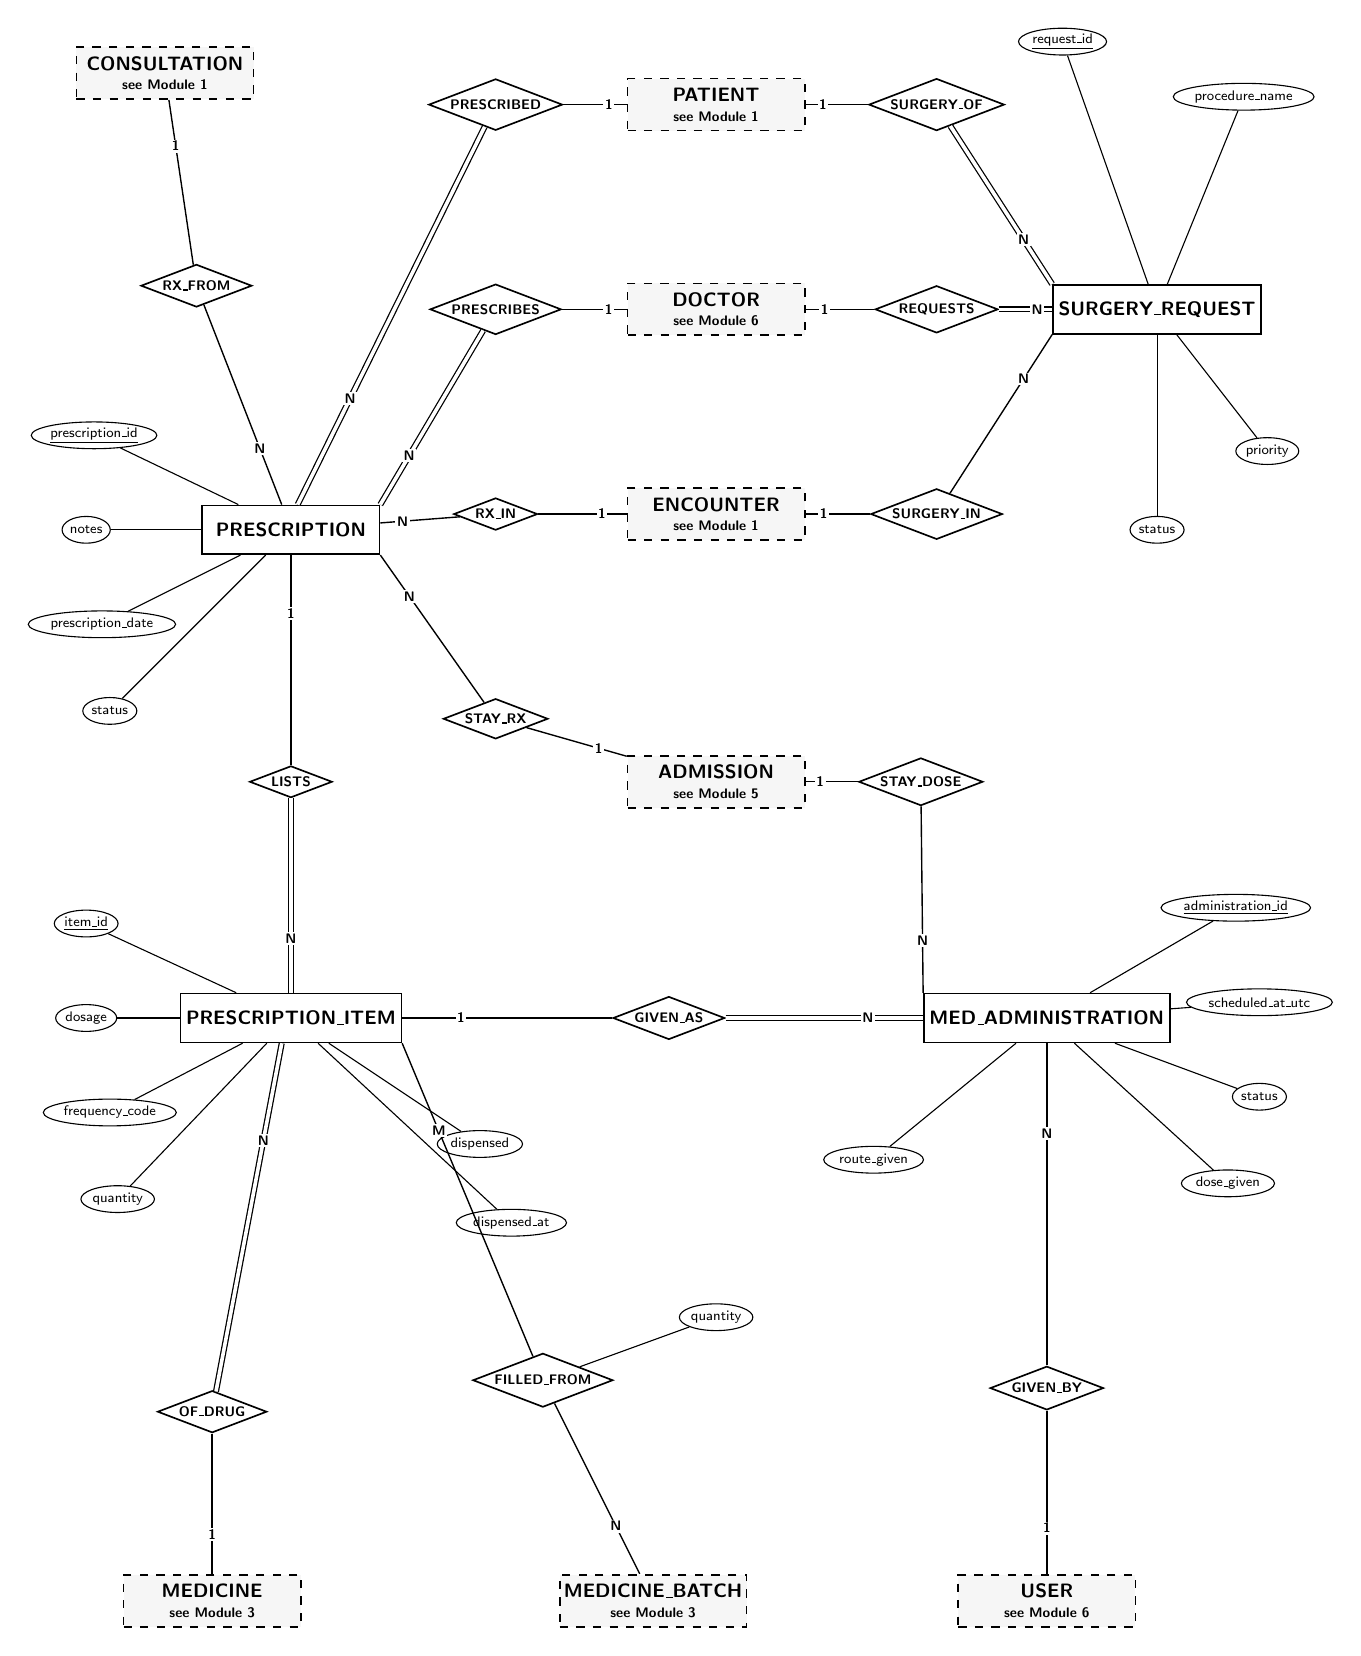
\begin{tikzpicture}[x=1cm,y=1cm]
\node[ent] (PRESCRIPTION) at (3.6,-7.4) {PRESCRIPTION};
\node[att] (PRESCRIPTION-prescription_id) at (1.1,-6.2) {\underline{prescription\_id}};
\draw (PRESCRIPTION-prescription_id) -- (PRESCRIPTION);
\node[att] (PRESCRIPTION-prescription_date) at (1.2,-8.6) {prescription\_date};
\draw (PRESCRIPTION-prescription_date) -- (PRESCRIPTION);
\node[att] (PRESCRIPTION-status) at (1.3,-9.7) {status};
\draw (PRESCRIPTION-status) -- (PRESCRIPTION);
\node[att] (PRESCRIPTION-notes) at (1,-7.4) {notes};
\draw (PRESCRIPTION-notes) -- (PRESCRIPTION);
\node[ent] (PRESCRIPTION_ITEM) at (3.6,-13.6) {PRESCRIPTION\_ITEM};
\node[att] (PRESCRIPTION_ITEM-item_id) at (1,-12.4) {\underline{item\_id}};
\draw (PRESCRIPTION_ITEM-item_id) -- (PRESCRIPTION_ITEM);
\node[att] (PRESCRIPTION_ITEM-dosage) at (1,-13.6) {dosage};
\draw (PRESCRIPTION_ITEM-dosage) -- (PRESCRIPTION_ITEM);
\node[att] (PRESCRIPTION_ITEM-frequency_code) at (1.3,-14.8) {frequency\_code};
\draw (PRESCRIPTION_ITEM-frequency_code) -- (PRESCRIPTION_ITEM);
\node[att] (PRESCRIPTION_ITEM-quantity) at (1.4,-15.9) {quantity};
\draw (PRESCRIPTION_ITEM-quantity) -- (PRESCRIPTION_ITEM);
\node[att] (PRESCRIPTION_ITEM-dispensed) at (6,-15.2) {dispensed};
\draw (PRESCRIPTION_ITEM-dispensed) -- (PRESCRIPTION_ITEM);
\node[att] (PRESCRIPTION_ITEM-dispensed_at) at (6.4,-16.2) {dispensed\_at};
\draw (PRESCRIPTION_ITEM-dispensed_at) -- (PRESCRIPTION_ITEM);
\node[ent] (MED_ADMINISTRATION) at (13.2,-13.6) {MED\_ADMINISTRATION};
\node[att] (MED_ADMINISTRATION-administration_id) at (15.6,-12.2) {\underline{administration\_id}};
\draw (MED_ADMINISTRATION-administration_id) -- (MED_ADMINISTRATION);
\node[att] (MED_ADMINISTRATION-scheduled_at_utc) at (15.9,-13.4) {scheduled\_at\_utc};
\draw (MED_ADMINISTRATION-scheduled_at_utc) -- (MED_ADMINISTRATION);
\node[att] (MED_ADMINISTRATION-status) at (15.9,-14.6) {status};
\draw (MED_ADMINISTRATION-status) -- (MED_ADMINISTRATION);
\node[att] (MED_ADMINISTRATION-dose_given) at (15.5,-15.7) {dose\_given};
\draw (MED_ADMINISTRATION-dose_given) -- (MED_ADMINISTRATION);
\node[att] (MED_ADMINISTRATION-route_given) at (11,-15.4) {route\_given};
\draw (MED_ADMINISTRATION-route_given) -- (MED_ADMINISTRATION);
\node[ent] (SURGERY_REQUEST) at (14.6,-4.6) {SURGERY\_REQUEST};
\node[att] (SURGERY_REQUEST-request_id) at (13.4,-1.2) {\underline{request\_id}};
\draw (SURGERY_REQUEST-request_id) -- (SURGERY_REQUEST);
\node[att] (SURGERY_REQUEST-procedure_name) at (15.7,-1.9) {procedure\_name};
\draw (SURGERY_REQUEST-procedure_name) -- (SURGERY_REQUEST);
\node[att] (SURGERY_REQUEST-priority) at (16,-6.4) {priority};
\draw (SURGERY_REQUEST-priority) -- (SURGERY_REQUEST);
\node[att] (SURGERY_REQUEST-status) at (14.6,-7.4) {status};
\draw (SURGERY_REQUEST-status) -- (SURGERY_REQUEST);
\node[refent] (PATIENT) at (9,-2) {PATIENT\\[-1pt]{\tiny see Module 1}};
\node[refent] (DOCTOR) at (9,-4.6) {DOCTOR\\[-1pt]{\tiny see Module 6}};
\node[refent] (ENCOUNTER) at (9,-7.2) {ENCOUNTER\\[-1pt]{\tiny see Module 1}};
\node[refent] (CONSULTATION) at (2,-1.6) {CONSULTATION\\[-1pt]{\tiny see Module 1}};
\node[refent] (ADMISSION) at (9,-10.6) {ADMISSION\\[-1pt]{\tiny see Module 5}};
\node[refent] (MEDICINE) at (2.6,-21) {MEDICINE\\[-1pt]{\tiny see Module 3}};
\node[refent] (MEDICINE_BATCH) at (8.2,-21) {MEDICINE\_BATCH\\[-1pt]{\tiny see Module 3}};
\node[refent] (USER) at (13.2,-21) {USER\\[-1pt]{\tiny see Module 6}};
\node[rel] (PRESCRIBED) at (6.2,-2) {PRESCRIBED};
\draw[partial] (PRESCRIBED) -- node[card,pos=0.72] {1} (PATIENT);
\draw[total] (PRESCRIBED) -- node[card,pos=0.72] {N} (PRESCRIPTION.75);
\node[rel] (PRESCRIBES) at (6.2,-4.6) {PRESCRIBES};
\draw[partial] (PRESCRIBES) -- node[card,pos=0.72] {1} (DOCTOR);
\draw[total] (PRESCRIBES) -- node[card,pos=0.72] {N} (PRESCRIPTION.north east);
\node[rel] (RX_IN) at (6.2,-7.2) {RX\_IN};
\draw[partial] (RX_IN) -- node[card,pos=0.72] {1} (ENCOUNTER);
\draw[partial] (RX_IN) -- node[card,pos=0.72] {N} (PRESCRIPTION);
\node[rel] (RX_FROM) at (2.4,-4.3) {RX\_FROM};
\draw[partial] (RX_FROM) -- node[card,pos=0.72] {1} (CONSULTATION);
\draw[partial] (RX_FROM) -- node[card,pos=0.72] {N} (PRESCRIPTION.110);
\node[rel] (STAY_RX) at (6.2,-9.8) {STAY\_RX};
\draw[partial] (STAY_RX) -- node[card,pos=0.72] {1} (ADMISSION);
\draw[partial] (STAY_RX) -- node[card,pos=0.72] {N} (PRESCRIPTION.south east);
\node[rel] (LISTS) at (3.6,-10.6) {LISTS};
\draw[partial] (LISTS) -- node[card,pos=0.72] {1} (PRESCRIPTION);
\draw[total] (LISTS) -- node[card,pos=0.72] {N} (PRESCRIPTION_ITEM);
\node[rel] (OF_DRUG) at (2.6,-18.6) {OF\_DRUG};
\draw[partial] (OF_DRUG) -- node[card,pos=0.72] {1} (MEDICINE);
\draw[total] (OF_DRUG) -- node[card,pos=0.72] {N} (PRESCRIPTION_ITEM.-110);
\node[rel] (FILLED_FROM) at (6.8,-18.2) {FILLED\_FROM};
\draw[partial] (FILLED_FROM) -- node[card,pos=0.72] {M} (PRESCRIPTION_ITEM.south east);
\draw[partial] (FILLED_FROM) -- node[card,pos=0.72] {N} (MEDICINE_BATCH);
\node[att] (FILLED_FROM-quantity) at (9,-17.4) {quantity};
\draw (FILLED_FROM-quantity) -- (FILLED_FROM);
\node[rel] (GIVEN_AS) at (8.4,-13.6) {GIVEN\_AS};
\draw[partial] (GIVEN_AS) -- node[card,pos=0.72] {1} (PRESCRIPTION_ITEM);
\draw[total] (GIVEN_AS) -- node[card,pos=0.72] {N} (MED_ADMINISTRATION);
\node[rel] (STAY_DOSE) at (11.6,-10.6) {STAY\_DOSE};
\draw[partial] (STAY_DOSE) -- node[card,pos=0.72] {1} (ADMISSION);
\draw[partial] (STAY_DOSE) -- node[card,pos=0.72] {N} (MED_ADMINISTRATION.north west);
\node[rel] (GIVEN_BY) at (13.2,-18.3) {GIVEN\_BY};
\draw[partial] (GIVEN_BY) -- node[card,pos=0.72] {1} (USER);
\draw[partial] (GIVEN_BY) -- node[card,pos=0.72] {N} (MED_ADMINISTRATION);
\node[rel] (SURGERY_OF) at (11.8,-2) {SURGERY\_OF};
\draw[partial] (SURGERY_OF) -- node[card,pos=0.72] {1} (PATIENT);
\draw[total] (SURGERY_OF) -- node[card,pos=0.72] {N} (SURGERY_REQUEST.north west);
\node[rel] (REQUESTS) at (11.8,-4.6) {REQUESTS};
\draw[partial] (REQUESTS) -- node[card,pos=0.72] {1} (DOCTOR);
\draw[total] (REQUESTS) -- node[card,pos=0.72] {N} (SURGERY_REQUEST);
\node[rel] (SURGERY_IN) at (11.8,-7.2) {SURGERY\_IN};
\draw[partial] (SURGERY_IN) -- node[card,pos=0.72] {1} (ENCOUNTER);
\draw[partial] (SURGERY_IN) -- node[card,pos=0.72] {N} (SURGERY_REQUEST.south west);
\end{tikzpicture}
\minilegend
\caption{Module 2, Clinical orders: prescriptions, prescription lines, medication administration and surgery requests}\label{fig:m2}
\end{figure}

\begin{figure}[p]\centering
% Generated by docs/report/gen/gen-er.js: diagram 4 (Module 4)
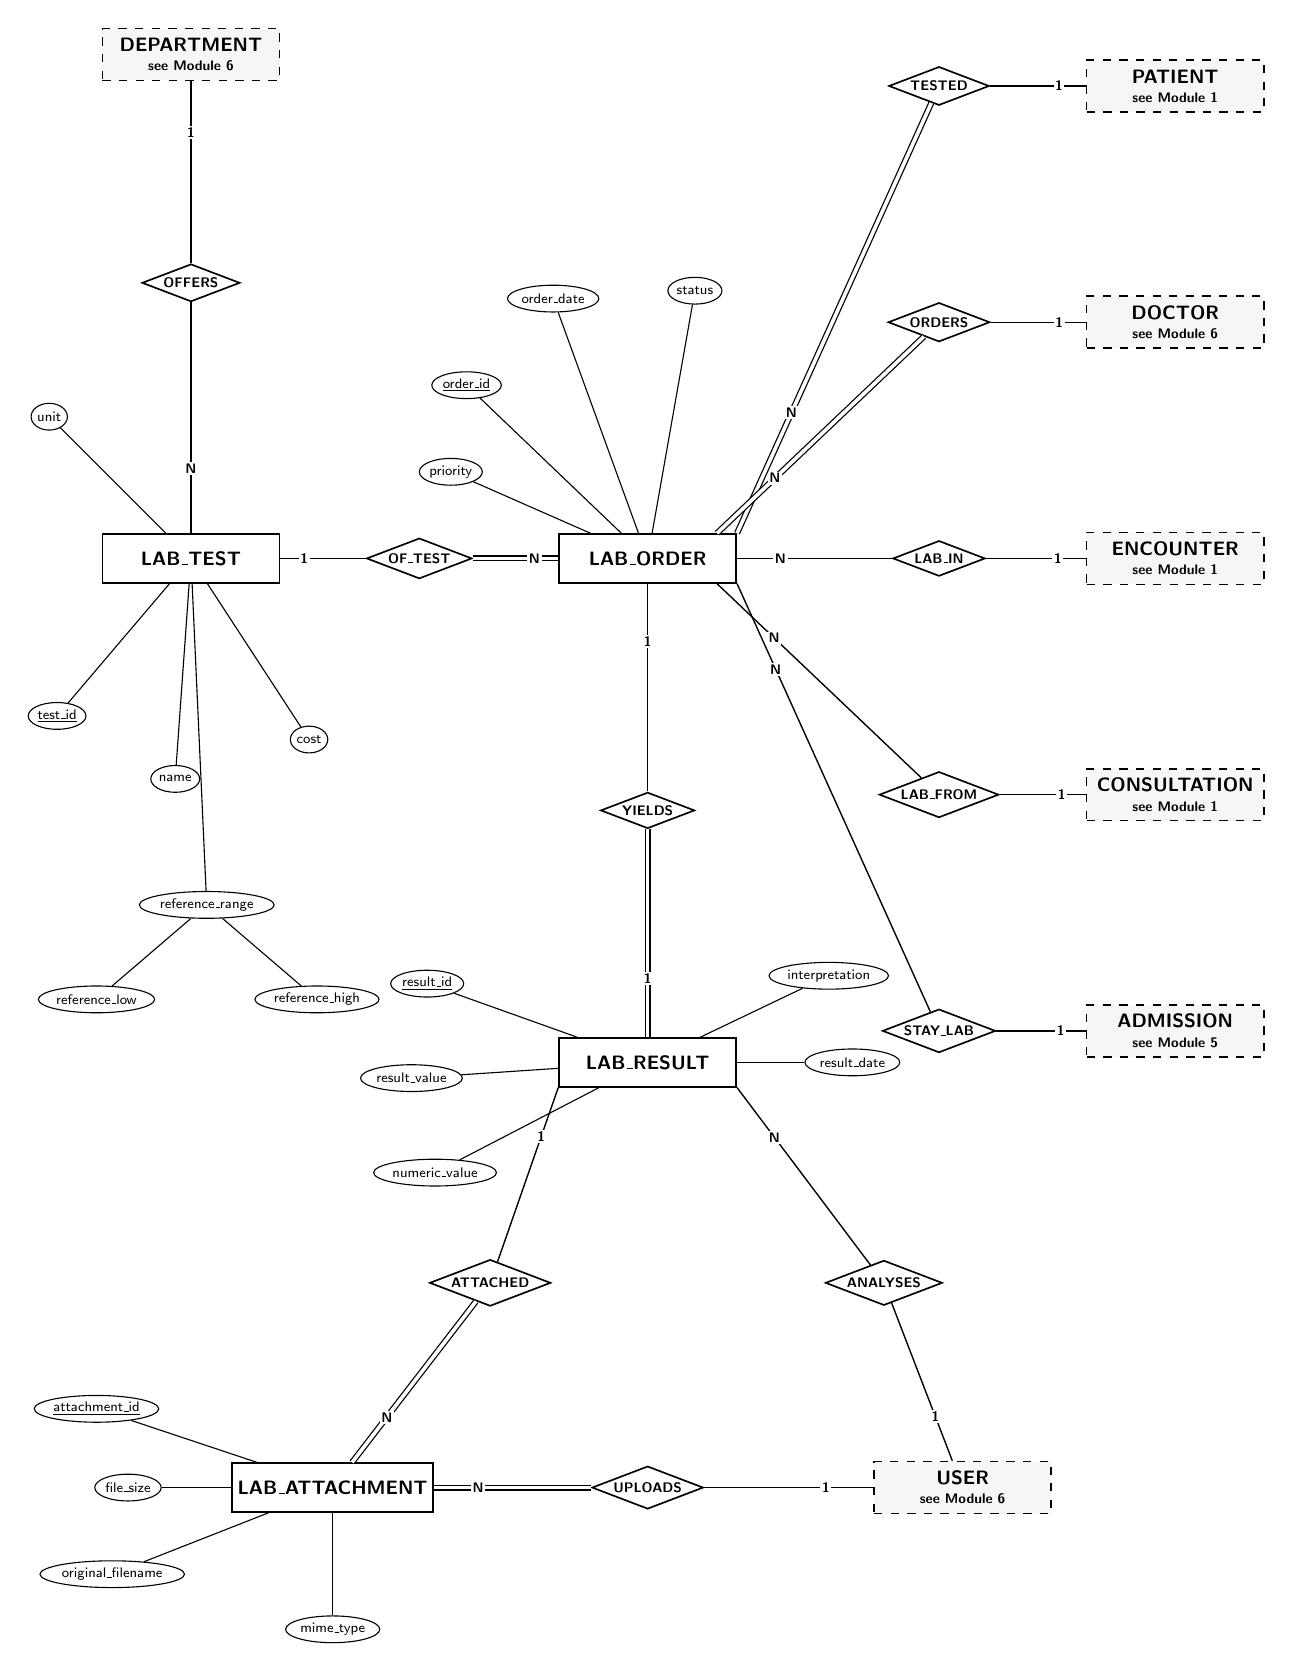
\begin{tikzpicture}[x=1cm,y=1cm]
\node[ent] (LAB_TEST) at (2.8,-8.6) {LAB\_TEST};
\node[att] (LAB_TEST-test_id) at (1.1,-10.6) {\underline{test\_id}};
\draw (LAB_TEST-test_id) -- (LAB_TEST);
\node[att] (LAB_TEST-name) at (2.6,-11.4) {name};
\draw (LAB_TEST-name) -- (LAB_TEST);
\node[att] (LAB_TEST-cost) at (4.3,-10.9) {cost};
\draw (LAB_TEST-cost) -- (LAB_TEST);
\node[att] (LAB_TEST-unit) at (1,-6.8) {unit};
\draw (LAB_TEST-unit) -- (LAB_TEST);
\node[att] (LAB_TEST-reference_range) at (3,-13) {reference\_range};
\draw (LAB_TEST-reference_range) -- (LAB_TEST);
\node[att] (LAB_TEST-reference_range-reference_low) at (1.6,-14.2) {reference\_low};
\draw (LAB_TEST-reference_range-reference_low) -- (LAB_TEST-reference_range);
\node[att] (LAB_TEST-reference_range-reference_high) at (4.4,-14.2) {reference\_high};
\draw (LAB_TEST-reference_range-reference_high) -- (LAB_TEST-reference_range);
\node[ent] (LAB_ORDER) at (8.6,-8.6) {LAB\_ORDER};
\node[att] (LAB_ORDER-order_id) at (6.3,-6.4) {\underline{order\_id}};
\draw (LAB_ORDER-order_id) -- (LAB_ORDER);
\node[att] (LAB_ORDER-order_date) at (7.4,-5.3) {order\_date};
\draw (LAB_ORDER-order_date) -- (LAB_ORDER);
\node[att] (LAB_ORDER-status) at (9.2,-5.2) {status};
\draw (LAB_ORDER-status) -- (LAB_ORDER);
\node[att] (LAB_ORDER-priority) at (6.1,-7.5) {priority};
\draw (LAB_ORDER-priority) -- (LAB_ORDER);
\node[ent] (LAB_RESULT) at (8.6,-15) {LAB\_RESULT};
\node[att] (LAB_RESULT-result_id) at (5.8,-14) {\underline{result\_id}};
\draw (LAB_RESULT-result_id) -- (LAB_RESULT);
\node[att] (LAB_RESULT-result_value) at (5.6,-15.2) {result\_value};
\draw (LAB_RESULT-result_value) -- (LAB_RESULT);
\node[att] (LAB_RESULT-numeric_value) at (5.9,-16.4) {numeric\_value};
\draw (LAB_RESULT-numeric_value) -- (LAB_RESULT);
\node[att] (LAB_RESULT-interpretation) at (10.9,-13.9) {interpretation};
\draw (LAB_RESULT-interpretation) -- (LAB_RESULT);
\node[att] (LAB_RESULT-result_date) at (11.2,-15) {result\_date};
\draw (LAB_RESULT-result_date) -- (LAB_RESULT);
\node[ent] (LAB_ATTACHMENT) at (4.6,-20.4) {LAB\_ATTACHMENT};
\node[att] (LAB_ATTACHMENT-attachment_id) at (1.6,-19.4) {\underline{attachment\_id}};
\draw (LAB_ATTACHMENT-attachment_id) -- (LAB_ATTACHMENT);
\node[att] (LAB_ATTACHMENT-original_filename) at (1.8,-21.5) {original\_filename};
\draw (LAB_ATTACHMENT-original_filename) -- (LAB_ATTACHMENT);
\node[att] (LAB_ATTACHMENT-mime_type) at (4.6,-22.2) {mime\_type};
\draw (LAB_ATTACHMENT-mime_type) -- (LAB_ATTACHMENT);
\node[att] (LAB_ATTACHMENT-file_size) at (2,-20.4) {file\_size};
\draw (LAB_ATTACHMENT-file_size) -- (LAB_ATTACHMENT);
\node[refent] (DEPARTMENT) at (2.8,-2.2) {DEPARTMENT\\[-1pt]{\tiny see Module 6}};
\node[refent] (PATIENT) at (15.3,-2.6) {PATIENT\\[-1pt]{\tiny see Module 1}};
\node[refent] (DOCTOR) at (15.3,-5.6) {DOCTOR\\[-1pt]{\tiny see Module 6}};
\node[refent] (ENCOUNTER) at (15.3,-8.6) {ENCOUNTER\\[-1pt]{\tiny see Module 1}};
\node[refent] (CONSULTATION) at (15.3,-11.6) {CONSULTATION\\[-1pt]{\tiny see Module 1}};
\node[refent] (ADMISSION) at (15.3,-14.6) {ADMISSION\\[-1pt]{\tiny see Module 5}};
\node[refent] (USER) at (12.6,-20.4) {USER\\[-1pt]{\tiny see Module 6}};
\node[rel] (OF_TEST) at (5.7,-8.6) {OF\_TEST};
\draw[partial] (OF_TEST) -- node[card,pos=0.72] {1} (LAB_TEST);
\draw[total] (OF_TEST) -- node[card,pos=0.72] {N} (LAB_ORDER);
\node[rel] (OFFERS) at (2.8,-5.1) {OFFERS};
\draw[partial] (OFFERS) -- node[card,pos=0.72] {1} (DEPARTMENT);
\draw[partial] (OFFERS) -- node[card,pos=0.72] {N} (LAB_TEST);
\node[rel] (TESTED) at (12.3,-2.6) {TESTED};
\draw[partial] (TESTED) -- node[card,pos=0.72] {1} (PATIENT);
\draw[total] (TESTED) -- node[card,pos=0.72] {N} (LAB_ORDER.north east);
\node[rel] (ORDERS) at (12.3,-5.6) {ORDERS};
\draw[partial] (ORDERS) -- node[card,pos=0.72] {1} (DOCTOR);
\draw[total] (ORDERS) -- node[card,pos=0.72] {N} (LAB_ORDER.20);
\node[rel] (LAB_IN) at (12.3,-8.6) {LAB\_IN};
\draw[partial] (LAB_IN) -- node[card,pos=0.72] {1} (ENCOUNTER);
\draw[partial] (LAB_IN) -- node[card,pos=0.72] {N} (LAB_ORDER);
\node[rel] (LAB_FROM) at (12.3,-11.6) {LAB\_FROM};
\draw[partial] (LAB_FROM) -- node[card,pos=0.72] {1} (CONSULTATION);
\draw[partial] (LAB_FROM) -- node[card,pos=0.72] {N} (LAB_ORDER.-20);
\node[rel] (STAY_LAB) at (12.3,-14.6) {STAY\_LAB};
\draw[partial] (STAY_LAB) -- node[card,pos=0.72] {1} (ADMISSION);
\draw[partial] (STAY_LAB) -- node[card,pos=0.8] {N} (LAB_ORDER.south east);
\node[rel] (YIELDS) at (8.6,-11.8) {YIELDS};
\draw[partial] (YIELDS) -- node[card,pos=0.72] {1} (LAB_ORDER);
\draw[total] (YIELDS) -- node[card,pos=0.72] {1} (LAB_RESULT);
\node[rel] (ANALYSES) at (11.6,-17.8) {ANALYSES};
\draw[partial] (ANALYSES) -- node[card,pos=0.72] {1} (USER);
\draw[partial] (ANALYSES) -- node[card,pos=0.72] {N} (LAB_RESULT.south east);
\node[rel] (ATTACHED) at (6.6,-17.8) {ATTACHED};
\draw[partial] (ATTACHED) -- node[card,pos=0.72] {1} (LAB_RESULT.south west);
\draw[total] (ATTACHED) -- node[card,pos=0.72] {N} (LAB_ATTACHMENT);
\node[rel] (UPLOADS) at (8.6,-20.4) {UPLOADS};
\draw[partial] (UPLOADS) -- node[card,pos=0.72] {1} (USER);
\draw[total] (UPLOADS) -- node[card,pos=0.72] {N} (LAB_ATTACHMENT);
\end{tikzpicture}
\minilegend
\caption{Module 4, Laboratory: tests, orders, results and report files}\label{fig:m4}
\end{figure}

\begin{figure}[p]\centering
% Generated by docs/report/gen/gen-er.js: diagram 5a (Module 5)
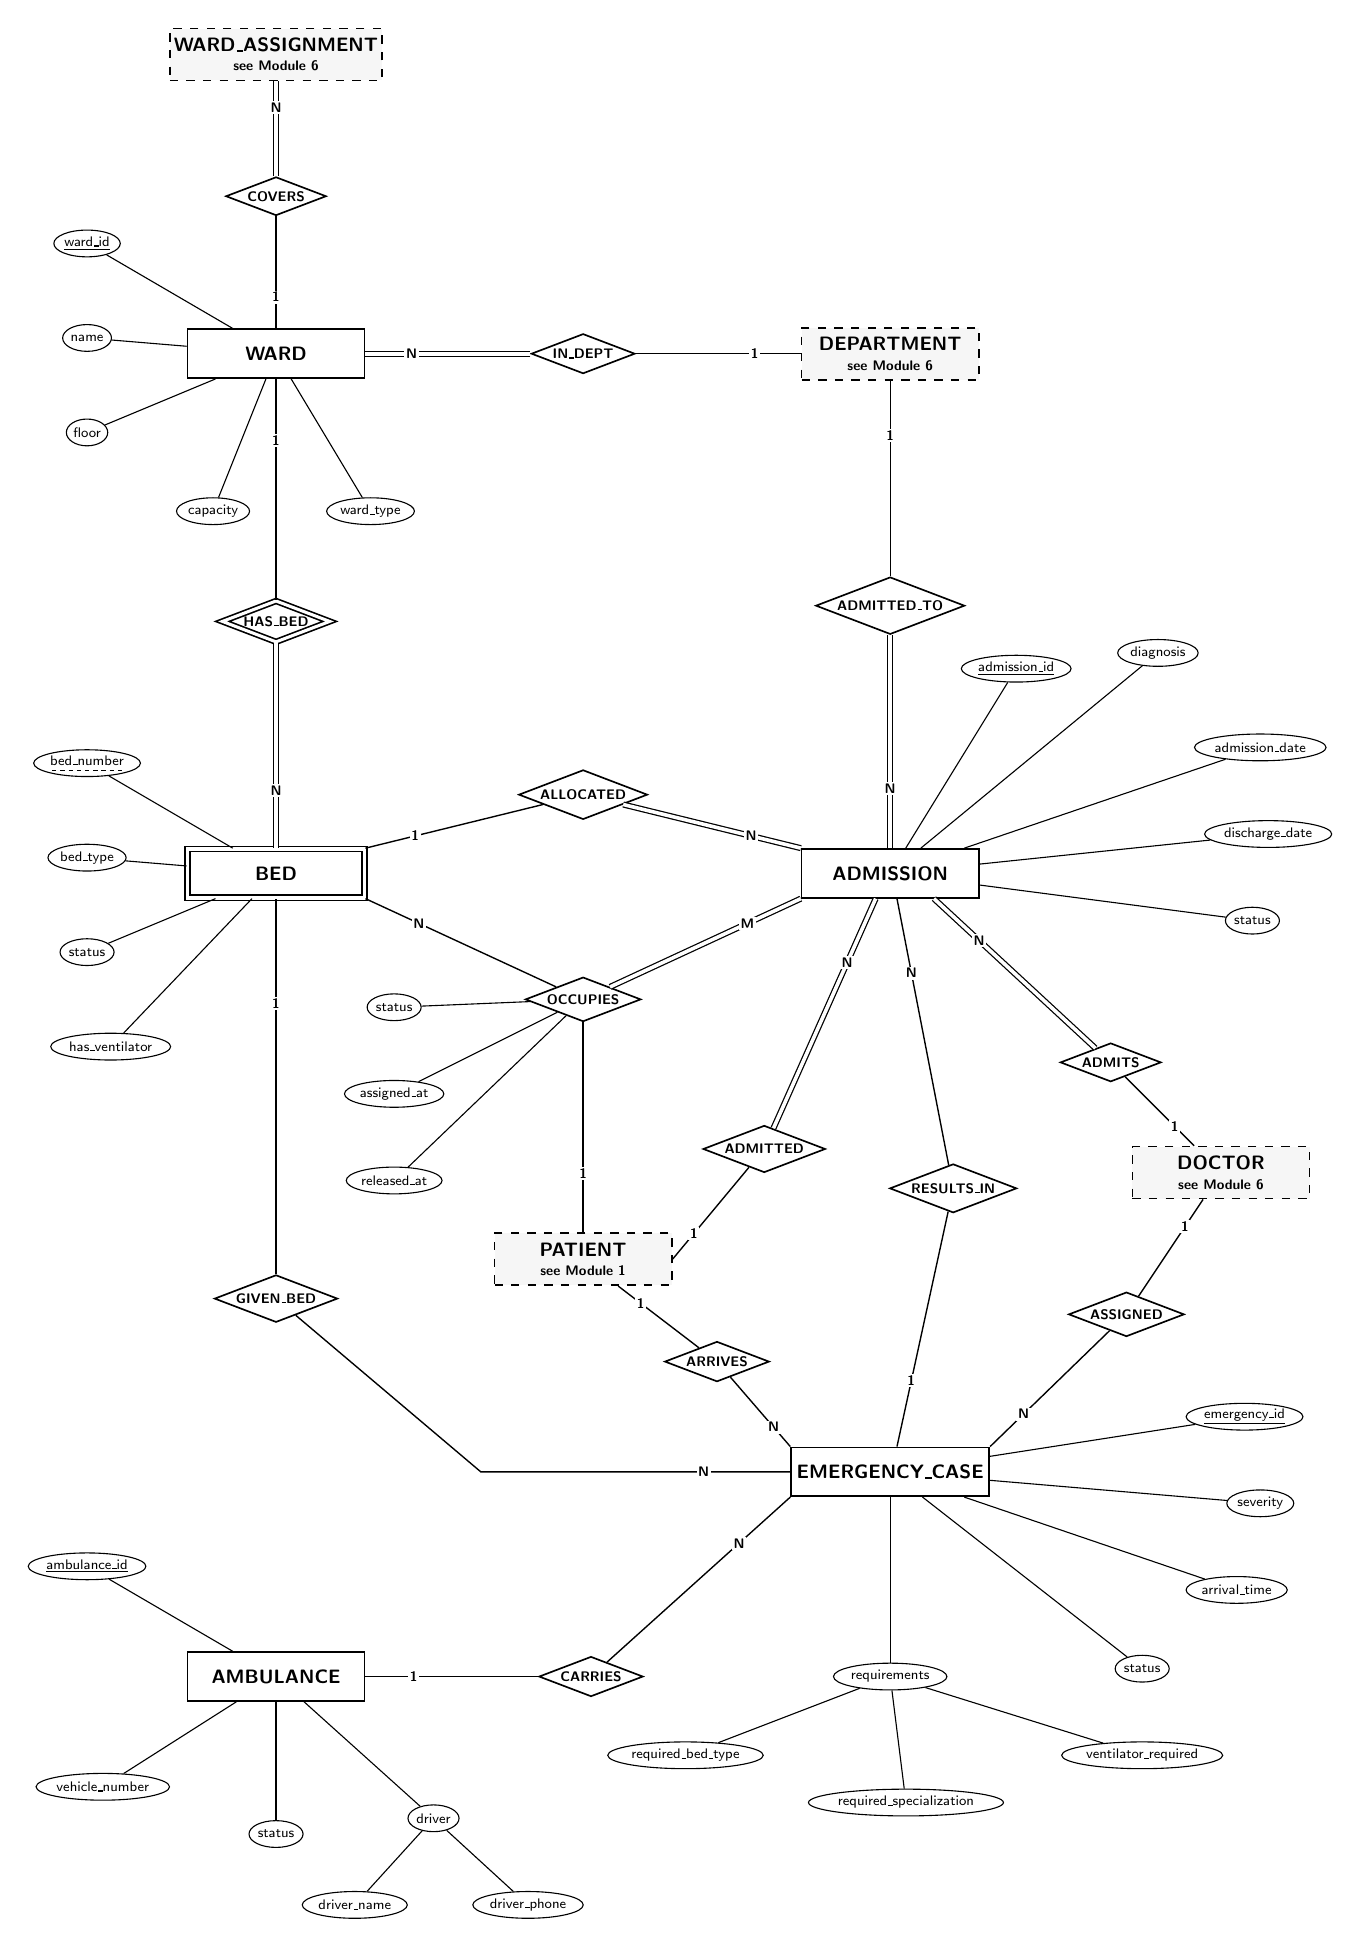
\begin{tikzpicture}[x=1cm,y=1cm]
\node[ent] (WARD) at (3.4,-4.4) {WARD};
\node[att] (WARD-ward_id) at (1,-3) {\underline{ward\_id}};
\draw (WARD-ward_id) -- (WARD);
\node[att] (WARD-name) at (1,-4.2) {name};
\draw (WARD-name) -- (WARD);
\node[att] (WARD-floor) at (1,-5.4) {floor};
\draw (WARD-floor) -- (WARD);
\node[att] (WARD-capacity) at (2.6,-6.4) {capacity};
\draw (WARD-capacity) -- (WARD);
\node[att] (WARD-ward_type) at (4.6,-6.4) {ward\_type};
\draw (WARD-ward_type) -- (WARD);
\node[weakent] (BED) at (3.4,-11) {BED};
\node[att] (BED-bed_number) at (1,-9.6) {\dashuline{bed\_number}};
\draw (BED-bed_number) -- (BED);
\node[att] (BED-bed_type) at (1,-10.8) {bed\_type};
\draw (BED-bed_type) -- (BED);
\node[att] (BED-status) at (1,-12) {status};
\draw (BED-status) -- (BED);
\node[att] (BED-has_ventilator) at (1.3,-13.2) {has\_ventilator};
\draw (BED-has_ventilator) -- (BED);
\node[ent] (ADMISSION) at (11.2,-11) {ADMISSION};
\node[att] (ADMISSION-admission_id) at (12.8,-8.4) {\underline{admission\_id}};
\draw (ADMISSION-admission_id) -- (ADMISSION);
\node[att] (ADMISSION-admission_date) at (15.9,-9.4) {admission\_date};
\draw (ADMISSION-admission_date) -- (ADMISSION);
\node[att] (ADMISSION-discharge_date) at (16,-10.5) {discharge\_date};
\draw (ADMISSION-discharge_date) -- (ADMISSION);
\node[att] (ADMISSION-status) at (15.8,-11.6) {status};
\draw (ADMISSION-status) -- (ADMISSION);
\node[att] (ADMISSION-diagnosis) at (14.6,-8.2) {diagnosis};
\draw (ADMISSION-diagnosis) -- (ADMISSION);
\node[ent] (EMERGENCY_CASE) at (11.2,-18.6) {EMERGENCY\_CASE};
\node[att] (EMERGENCY_CASE-emergency_id) at (15.7,-17.9) {\underline{emergency\_id}};
\draw (EMERGENCY_CASE-emergency_id) -- (EMERGENCY_CASE);
\node[att] (EMERGENCY_CASE-severity) at (15.9,-19) {severity};
\draw (EMERGENCY_CASE-severity) -- (EMERGENCY_CASE);
\node[att] (EMERGENCY_CASE-arrival_time) at (15.6,-20.1) {arrival\_time};
\draw (EMERGENCY_CASE-arrival_time) -- (EMERGENCY_CASE);
\node[att] (EMERGENCY_CASE-status) at (14.4,-21.1) {status};
\draw (EMERGENCY_CASE-status) -- (EMERGENCY_CASE);
\node[att] (EMERGENCY_CASE-requirements) at (11.2,-21.2) {requirements};
\draw (EMERGENCY_CASE-requirements) -- (EMERGENCY_CASE);
\node[att] (EMERGENCY_CASE-requirements-required_bed_type) at (8.6,-22.2) {required\_bed\_type};
\draw (EMERGENCY_CASE-requirements-required_bed_type) -- (EMERGENCY_CASE-requirements);
\node[att] (EMERGENCY_CASE-requirements-required_specialization) at (11.4,-22.8) {required\_specialization};
\draw (EMERGENCY_CASE-requirements-required_specialization) -- (EMERGENCY_CASE-requirements);
\node[att] (EMERGENCY_CASE-requirements-ventilator_required) at (14.4,-22.2) {ventilator\_required};
\draw (EMERGENCY_CASE-requirements-ventilator_required) -- (EMERGENCY_CASE-requirements);
\node[ent] (AMBULANCE) at (3.4,-21.2) {AMBULANCE};
\node[att] (AMBULANCE-ambulance_id) at (1,-19.8) {\underline{ambulance\_id}};
\draw (AMBULANCE-ambulance_id) -- (AMBULANCE);
\node[att] (AMBULANCE-vehicle_number) at (1.2,-22.6) {vehicle\_number};
\draw (AMBULANCE-vehicle_number) -- (AMBULANCE);
\node[att] (AMBULANCE-driver) at (5.4,-23) {driver};
\draw (AMBULANCE-driver) -- (AMBULANCE);
\node[att] (AMBULANCE-driver-driver_name) at (4.4,-24.1) {driver\_name};
\draw (AMBULANCE-driver-driver_name) -- (AMBULANCE-driver);
\node[att] (AMBULANCE-driver-driver_phone) at (6.6,-24.1) {driver\_phone};
\draw (AMBULANCE-driver-driver_phone) -- (AMBULANCE-driver);
\node[att] (AMBULANCE-status) at (3.4,-23.2) {status};
\draw (AMBULANCE-status) -- (AMBULANCE);
\node[refent] (DEPARTMENT) at (11.2,-4.4) {DEPARTMENT\\[-1pt]{\tiny see Module 6}};
\node[refent] (WARD_ASSIGNMENT) at (3.4,-0.6) {WARD\_ASSIGNMENT\\[-1pt]{\tiny see Module 6}};
\node[refent] (PATIENT) at (7.3,-15.9) {PATIENT\\[-1pt]{\tiny see Module 1}};
\node[refent] (DOCTOR) at (15.4,-14.8) {DOCTOR\\[-1pt]{\tiny see Module 6}};
\node[idrel] (HAS_BED) at (3.4,-7.8) {HAS\_BED};
\draw[partial] (HAS_BED) -- node[card,pos=0.72] {1} (WARD);
\draw[total] (HAS_BED) -- node[card,pos=0.72] {N} (BED);
\node[rel] (IN_DEPT) at (7.3,-4.4) {IN\_DEPT};
\draw[partial] (IN_DEPT) -- node[card,pos=0.72] {1} (DEPARTMENT);
\draw[total] (IN_DEPT) -- node[card,pos=0.72] {N} (WARD);
\node[rel] (ADMITTED) at (9.6,-14.5) {ADMITTED};
\draw[partial] (ADMITTED) -- node[card,pos=0.72] {1} (PATIENT.east);
\draw[total] (ADMITTED) -- node[card,pos=0.72] {N} (ADMISSION.-120);
\node[rel] (ADMITS) at (14,-13.4) {ADMITS};
\draw[partial] (ADMITS) -- node[card,pos=0.72] {1} (DOCTOR);
\draw[total] (ADMITS) -- node[card,pos=0.72] {N} (ADMISSION.-30);
\node[rel] (ADMITTED_TO) at (11.2,-7.6) {ADMITTED\_TO};
\draw[partial] (ADMITTED_TO) -- node[card,pos=0.72] {1} (DEPARTMENT);
\draw[total] (ADMITTED_TO) -- node[card,pos=0.72] {N} (ADMISSION);
\node[rel] (ALLOCATED) at (7.3,-10) {ALLOCATED};
\draw[partial] (ALLOCATED) -- node[card,pos=0.72] {1} (BED.north east);
\draw[total] (ALLOCATED) -- node[card,pos=0.72] {N} (ADMISSION.north west);
\node[rel] (OCCUPIES) at (7.3,-12.6) {OCCUPIES};
\draw[partial] (OCCUPIES) -- node[card,pos=0.72] {N} (BED.south east);
\draw[total] (OCCUPIES) -- node[card,pos=0.72] {M} (ADMISSION.south west);
\draw[partial] (OCCUPIES) -- node[card,pos=0.72] {1} (PATIENT);
\node[att] (OCCUPIES-assigned_at) at (4.9,-13.8) {assigned\_at};
\draw (OCCUPIES-assigned_at) -- (OCCUPIES);
\node[att] (OCCUPIES-released_at) at (4.9,-14.9) {released\_at};
\draw (OCCUPIES-released_at) -- (OCCUPIES);
\node[att] (OCCUPIES-status) at (4.9,-12.7) {status};
\draw (OCCUPIES-status) -- (OCCUPIES);
\node[rel] (RESULTS_IN) at (12,-15) {RESULTS\_IN};
\draw[partial] (RESULTS_IN) -- node[card,pos=0.72] {1} (EMERGENCY_CASE.75);
\draw[partial] (RESULTS_IN) -- node[card,pos=0.72] {N} (ADMISSION.-75);
\node[rel] (ARRIVES) at (9,-17.2) {ARRIVES};
\draw[partial] (ARRIVES) -- node[card,pos=0.72] {1} (PATIENT);
\draw[partial] (ARRIVES) -- node[card,pos=0.72] {N} (EMERGENCY_CASE.north west);
\node[rel] (CARRIES) at (7.4,-21.2) {CARRIES};
\draw[partial] (CARRIES) -- node[card,pos=0.72] {1} (AMBULANCE);
\draw[partial] (CARRIES) -- node[card,pos=0.72] {N} (EMERGENCY_CASE.south west);
\node[rel] (ASSIGNED) at (14.2,-16.6) {ASSIGNED};
\draw[partial] (ASSIGNED) -- node[card,pos=0.72] {1} (DOCTOR);
\draw[partial] (ASSIGNED) -- node[card,pos=0.72] {N} (EMERGENCY_CASE.north east);
\node[rel] (GIVEN_BED) at (3.4,-16.4) {GIVEN\_BED};
\draw[partial] (GIVEN_BED) -- node[card,pos=0.72] {1} (BED.south);
\draw[partial] (GIVEN_BED) -- (6,-18.6) -- node[card,pos=0.72] {N} (EMERGENCY_CASE.west);
\node[rel] (COVERS) at (3.4,-2.4) {COVERS};
\draw[partial] (COVERS) -- node[card,pos=0.72] {1} (WARD);
\draw[total] (COVERS) -- node[card,pos=0.72] {N} (WARD_ASSIGNMENT);
\end{tikzpicture}
\minilegend
\caption{Module 5, Beds and admissions (page 1 of 2): wards, beds, admissions, emergencies and ambulances}\label{fig:m5a}
\end{figure}

\begin{figure}[p]\centering
% Generated by docs/report/gen/gen-er.js: diagram 5b (Module 5)
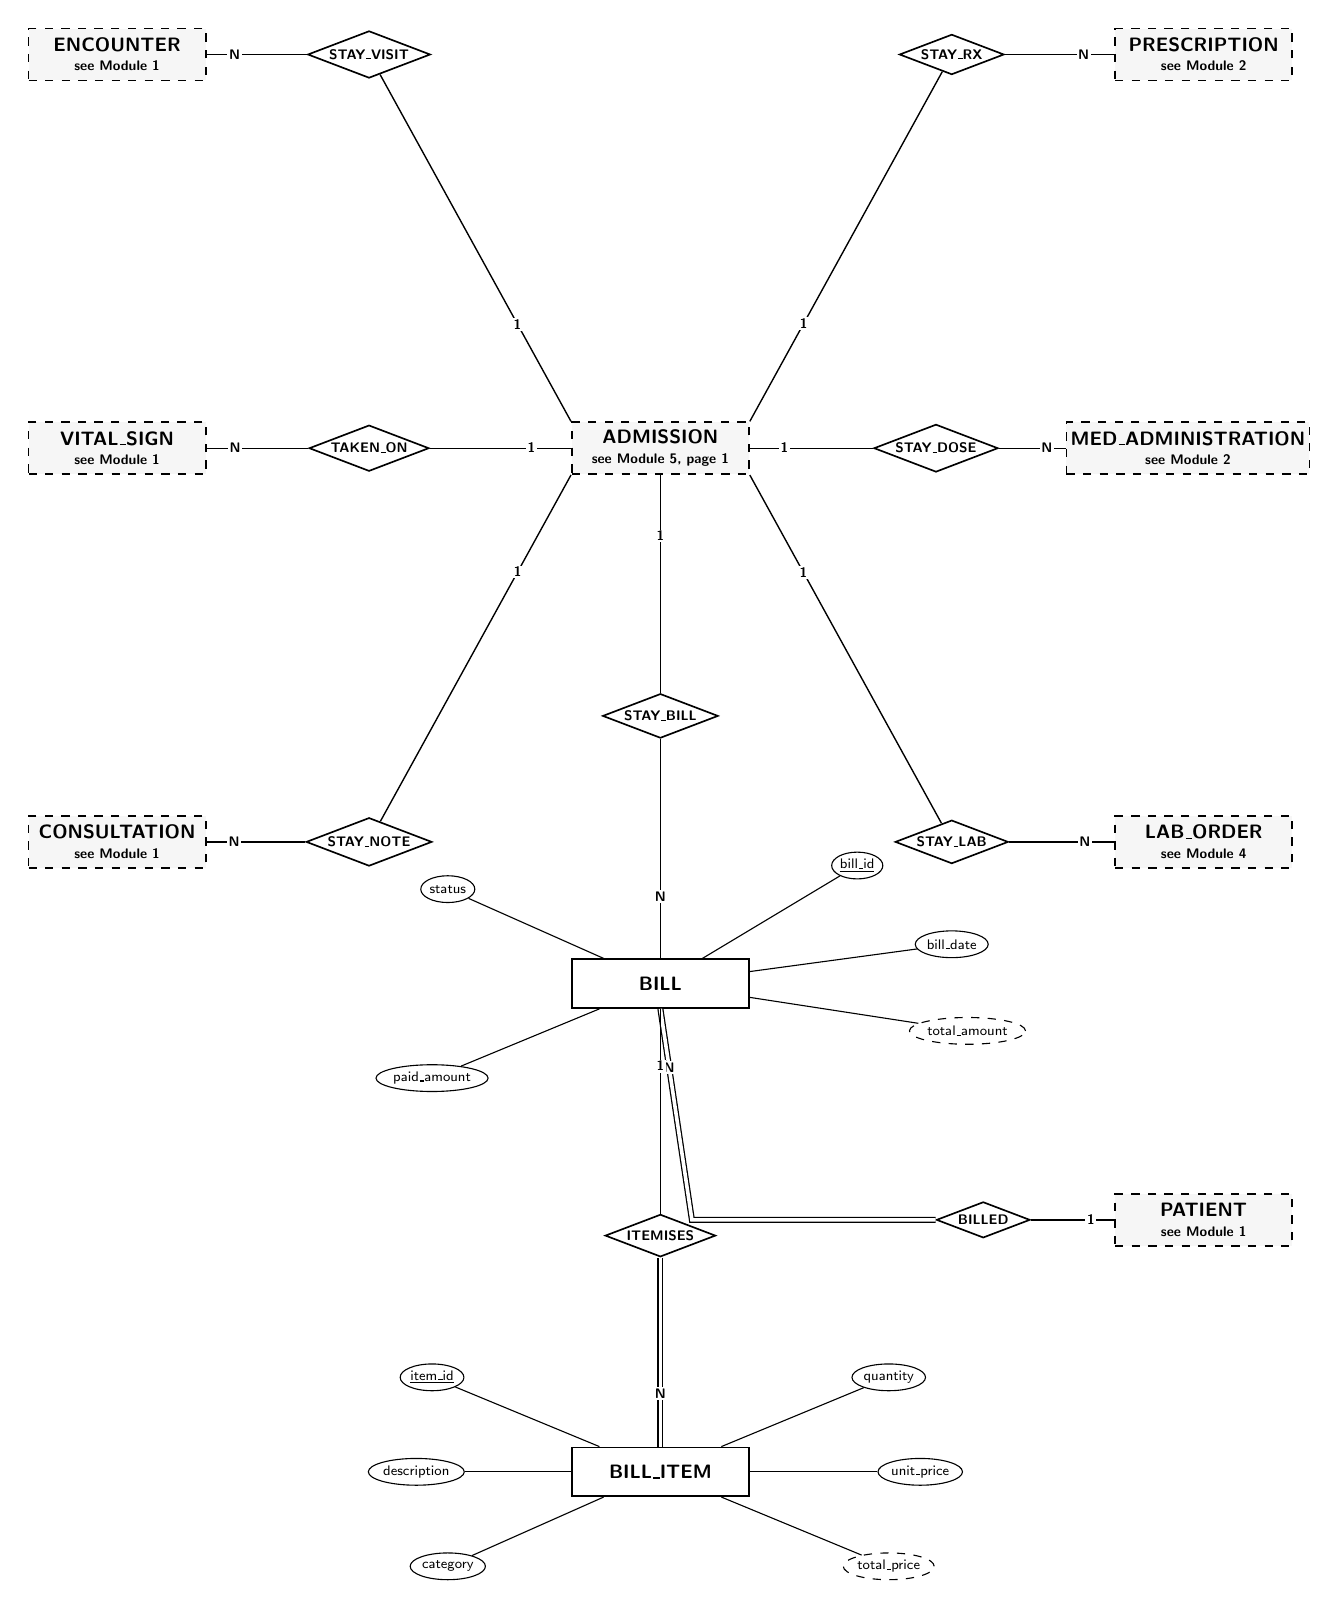
\begin{tikzpicture}[x=1cm,y=1cm]
\node[refent] (ADMISSION) at (8.5,-7.6) {ADMISSION\\[-1pt]{\tiny see Module 5, page 1}};
\node[ent] (BILL) at (8.5,-14.4) {BILL};
\node[att] (BILL-bill_id) at (11,-12.9) {\underline{bill\_id}};
\draw (BILL-bill_id) -- (BILL);
\node[att] (BILL-bill_date) at (12.2,-13.9) {bill\_date};
\draw (BILL-bill_date) -- (BILL);
\node[att,dashed] (BILL-total_amount) at (12.4,-15) {total\_amount};
\draw (BILL-total_amount) -- (BILL);
\node[att] (BILL-paid_amount) at (5.6,-15.6) {paid\_amount};
\draw (BILL-paid_amount) -- (BILL);
\node[att] (BILL-status) at (5.8,-13.2) {status};
\draw (BILL-status) -- (BILL);
\node[ent] (BILL_ITEM) at (8.5,-20.6) {BILL\_ITEM};
\node[att] (BILL_ITEM-item_id) at (5.6,-19.4) {\underline{item\_id}};
\draw (BILL_ITEM-item_id) -- (BILL_ITEM);
\node[att] (BILL_ITEM-description) at (5.4,-20.6) {description};
\draw (BILL_ITEM-description) -- (BILL_ITEM);
\node[att] (BILL_ITEM-category) at (5.8,-21.8) {category};
\draw (BILL_ITEM-category) -- (BILL_ITEM);
\node[att] (BILL_ITEM-quantity) at (11.4,-19.4) {quantity};
\draw (BILL_ITEM-quantity) -- (BILL_ITEM);
\node[att] (BILL_ITEM-unit_price) at (11.8,-20.6) {unit\_price};
\draw (BILL_ITEM-unit_price) -- (BILL_ITEM);
\node[att,dashed] (BILL_ITEM-total_price) at (11.4,-21.8) {total\_price};
\draw (BILL_ITEM-total_price) -- (BILL_ITEM);
\node[refent] (ENCOUNTER) at (1.6,-2.6) {ENCOUNTER\\[-1pt]{\tiny see Module 1}};
\node[refent] (VITAL_SIGN) at (1.6,-7.6) {VITAL\_SIGN\\[-1pt]{\tiny see Module 1}};
\node[refent] (CONSULTATION) at (1.6,-12.6) {CONSULTATION\\[-1pt]{\tiny see Module 1}};
\node[refent] (PRESCRIPTION) at (15.4,-2.6) {PRESCRIPTION\\[-1pt]{\tiny see Module 2}};
\node[refent] (MED_ADMINISTRATION) at (15.2,-7.6) {MED\_ADMINISTRATION\\[-1pt]{\tiny see Module 2}};
\node[refent] (LAB_ORDER) at (15.4,-12.6) {LAB\_ORDER\\[-1pt]{\tiny see Module 4}};
\node[refent] (PATIENT) at (15.4,-17.4) {PATIENT\\[-1pt]{\tiny see Module 1}};
\node[rel] (STAY_VISIT) at (4.8,-2.6) {STAY\_VISIT};
\draw[partial] (STAY_VISIT) -- node[card,pos=0.72] {1} (ADMISSION.north west);
\draw[partial] (STAY_VISIT) -- node[card,pos=0.72] {N} (ENCOUNTER);
\node[rel] (TAKEN_ON) at (4.8,-7.6) {TAKEN\_ON};
\draw[partial] (TAKEN_ON) -- node[card,pos=0.72] {1} (ADMISSION);
\draw[partial] (TAKEN_ON) -- node[card,pos=0.72] {N} (VITAL_SIGN);
\node[rel] (STAY_NOTE) at (4.8,-12.6) {STAY\_NOTE};
\draw[partial] (STAY_NOTE) -- node[card,pos=0.72] {1} (ADMISSION.south west);
\draw[partial] (STAY_NOTE) -- node[card,pos=0.72] {N} (CONSULTATION);
\node[rel] (STAY_RX) at (12.2,-2.6) {STAY\_RX};
\draw[partial] (STAY_RX) -- node[card,pos=0.72] {1} (ADMISSION.north east);
\draw[partial] (STAY_RX) -- node[card,pos=0.72] {N} (PRESCRIPTION);
\node[rel] (STAY_DOSE) at (12,-7.6) {STAY\_DOSE};
\draw[partial] (STAY_DOSE) -- node[card,pos=0.72] {1} (ADMISSION);
\draw[partial] (STAY_DOSE) -- node[card,pos=0.72] {N} (MED_ADMINISTRATION);
\node[rel] (STAY_LAB) at (12.2,-12.6) {STAY\_LAB};
\draw[partial] (STAY_LAB) -- node[card,pos=0.72] {1} (ADMISSION.south east);
\draw[partial] (STAY_LAB) -- node[card,pos=0.72] {N} (LAB_ORDER);
\node[rel] (BILLED) at (12.6,-17.4) {BILLED};
\draw[partial] (BILLED) -- node[card,pos=0.72] {1} (PATIENT);
\draw[total] (BILLED) -- (8.9,-17.4) -- node[card,pos=0.72] {N} (BILL.south);
\node[rel] (STAY_BILL) at (8.5,-11) {STAY\_BILL};
\draw[partial] (STAY_BILL) -- node[card,pos=0.72] {1} (ADMISSION);
\draw[partial] (STAY_BILL) -- node[card,pos=0.72] {N} (BILL);
\node[rel] (ITEMISES) at (8.5,-17.6) {ITEMISES};
\draw[partial] (ITEMISES) -- node[card,pos=0.72] {1} (BILL);
\draw[total] (ITEMISES) -- node[card,pos=0.72] {N} (BILL_ITEM);
\end{tikzpicture}
\minilegend
\caption{Module 5, Beds and admissions (page 2 of 2): what an admission covers, and billing}\label{fig:m5b}
\end{figure}

\begin{figure}[p]\centering
% Generated by docs/report/gen/gen-er.js: diagram 6a (Module 6)
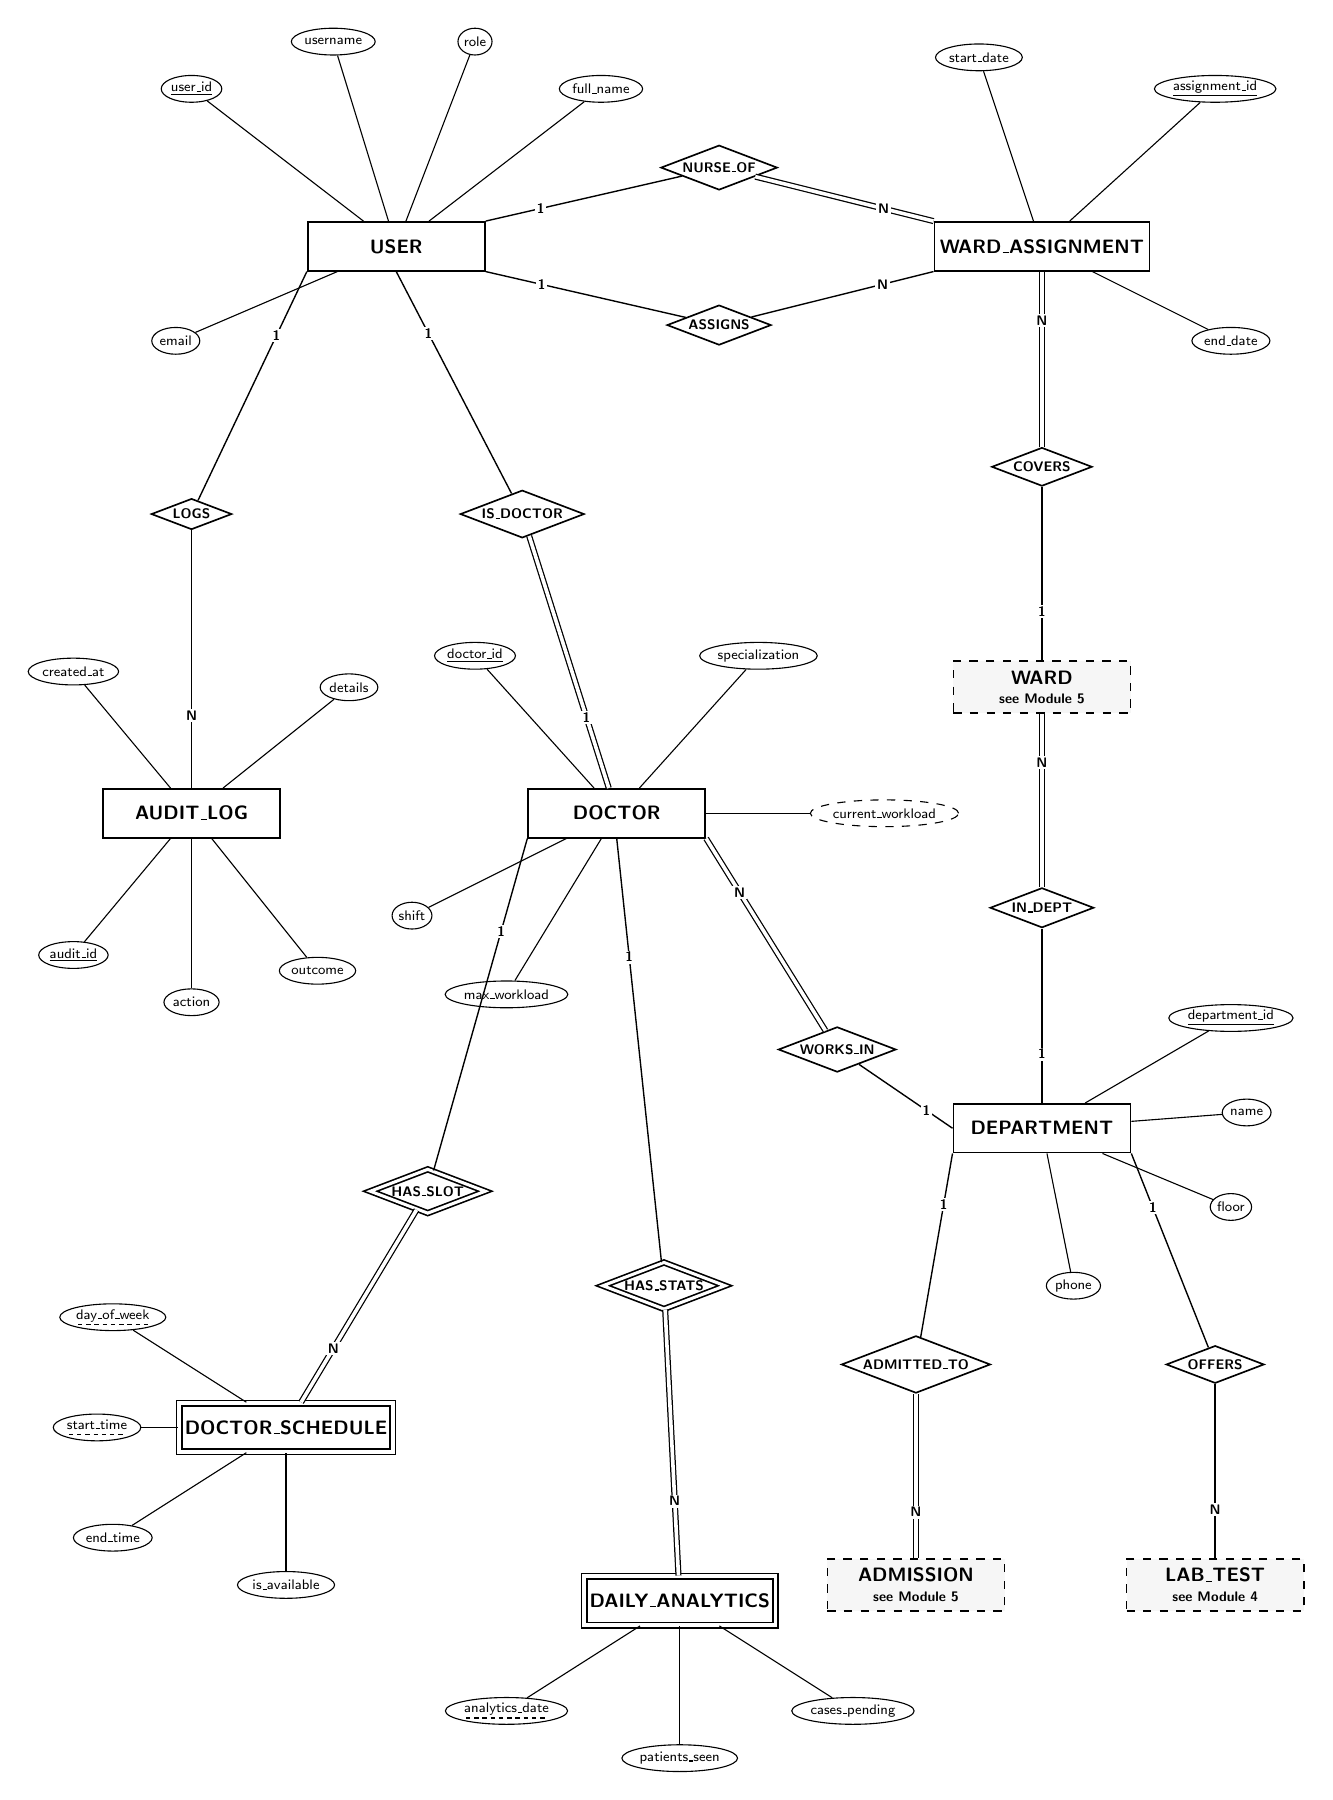
\begin{tikzpicture}[x=1cm,y=1cm]
\node[ent] (USER) at (5,-3.4) {USER};
\node[att] (USER-user_id) at (2.4,-1.4) {\underline{user\_id}};
\draw (USER-user_id) -- (USER);
\node[att] (USER-username) at (4.2,-0.8) {username};
\draw (USER-username) -- (USER);
\node[att] (USER-role) at (6,-0.8) {role};
\draw (USER-role) -- (USER);
\node[att] (USER-full_name) at (7.6,-1.4) {full\_name};
\draw (USER-full_name) -- (USER);
\node[att] (USER-email) at (2.2,-4.6) {email};
\draw (USER-email) -- (USER);
\node[ent] (WARD_ASSIGNMENT) at (13.2,-3.4) {WARD\_ASSIGNMENT};
\node[att] (WARD_ASSIGNMENT-assignment_id) at (15.4,-1.4) {\underline{assignment\_id}};
\draw (WARD_ASSIGNMENT-assignment_id) -- (WARD_ASSIGNMENT);
\node[att] (WARD_ASSIGNMENT-start_date) at (12.4,-1) {start\_date};
\draw (WARD_ASSIGNMENT-start_date) -- (WARD_ASSIGNMENT);
\node[att] (WARD_ASSIGNMENT-end_date) at (15.6,-4.6) {end\_date};
\draw (WARD_ASSIGNMENT-end_date) -- (WARD_ASSIGNMENT);
\node[ent] (AUDIT_LOG) at (2.4,-10.6) {AUDIT\_LOG};
\node[att] (AUDIT_LOG-audit_id) at (0.9,-12.4) {\underline{audit\_id}};
\draw (AUDIT_LOG-audit_id) -- (AUDIT_LOG);
\node[att] (AUDIT_LOG-action) at (2.4,-13) {action};
\draw (AUDIT_LOG-action) -- (AUDIT_LOG);
\node[att] (AUDIT_LOG-outcome) at (4,-12.6) {outcome};
\draw (AUDIT_LOG-outcome) -- (AUDIT_LOG);
\node[att] (AUDIT_LOG-created_at) at (0.9,-8.8) {created\_at};
\draw (AUDIT_LOG-created_at) -- (AUDIT_LOG);
\node[att] (AUDIT_LOG-details) at (4.4,-9) {details};
\draw (AUDIT_LOG-details) -- (AUDIT_LOG);
\node[ent] (DOCTOR) at (7.8,-10.6) {DOCTOR};
\node[att] (DOCTOR-doctor_id) at (6,-8.6) {\underline{doctor\_id}};
\draw (DOCTOR-doctor_id) -- (DOCTOR);
\node[att] (DOCTOR-specialization) at (9.6,-8.6) {specialization};
\draw (DOCTOR-specialization) -- (DOCTOR);
\node[att] (DOCTOR-shift) at (5.2,-11.9) {shift};
\draw (DOCTOR-shift) -- (DOCTOR);
\node[att] (DOCTOR-max_workload) at (6.4,-12.9) {max\_workload};
\draw (DOCTOR-max_workload) -- (DOCTOR);
\node[att,dashed] (DOCTOR-current_workload) at (11.2,-10.6) {current\_workload};
\draw (DOCTOR-current_workload) -- (DOCTOR);
\node[ent] (DEPARTMENT) at (13.2,-14.6) {DEPARTMENT};
\node[att] (DEPARTMENT-department_id) at (15.6,-13.2) {\underline{department\_id}};
\draw (DEPARTMENT-department_id) -- (DEPARTMENT);
\node[att] (DEPARTMENT-name) at (15.8,-14.4) {name};
\draw (DEPARTMENT-name) -- (DEPARTMENT);
\node[att] (DEPARTMENT-floor) at (15.6,-15.6) {floor};
\draw (DEPARTMENT-floor) -- (DEPARTMENT);
\node[att] (DEPARTMENT-phone) at (13.6,-16.6) {phone};
\draw (DEPARTMENT-phone) -- (DEPARTMENT);
\node[weakent] (DOCTOR_SCHEDULE) at (3.6,-18.4) {DOCTOR\_SCHEDULE};
\node[att] (DOCTOR_SCHEDULE-day_of_week) at (1.4,-17) {\dashuline{day\_of\_week}};
\draw (DOCTOR_SCHEDULE-day_of_week) -- (DOCTOR_SCHEDULE);
\node[att] (DOCTOR_SCHEDULE-start_time) at (1.2,-18.4) {\dashuline{start\_time}};
\draw (DOCTOR_SCHEDULE-start_time) -- (DOCTOR_SCHEDULE);
\node[att] (DOCTOR_SCHEDULE-end_time) at (1.4,-19.8) {end\_time};
\draw (DOCTOR_SCHEDULE-end_time) -- (DOCTOR_SCHEDULE);
\node[att] (DOCTOR_SCHEDULE-is_available) at (3.6,-20.4) {is\_available};
\draw (DOCTOR_SCHEDULE-is_available) -- (DOCTOR_SCHEDULE);
\node[weakent] (DAILY_ANALYTICS) at (8.6,-20.6) {DAILY\_ANALYTICS};
\node[att] (DAILY_ANALYTICS-analytics_date) at (6.4,-22) {\dashuline{analytics\_date}};
\draw (DAILY_ANALYTICS-analytics_date) -- (DAILY_ANALYTICS);
\node[att] (DAILY_ANALYTICS-patients_seen) at (8.6,-22.6) {patients\_seen};
\draw (DAILY_ANALYTICS-patients_seen) -- (DAILY_ANALYTICS);
\node[att] (DAILY_ANALYTICS-cases_pending) at (10.8,-22) {cases\_pending};
\draw (DAILY_ANALYTICS-cases_pending) -- (DAILY_ANALYTICS);
\node[refent] (WARD) at (13.2,-9) {WARD\\[-1pt]{\tiny see Module 5}};
\node[refent] (LAB_TEST) at (15.4,-20.4) {LAB\_TEST\\[-1pt]{\tiny see Module 4}};
\node[refent] (ADMISSION) at (11.6,-20.4) {ADMISSION\\[-1pt]{\tiny see Module 5}};
\node[rel] (OFFERS) at (15.4,-17.6) {OFFERS};
\draw[partial] (OFFERS) -- node[card,pos=0.72] {1} (DEPARTMENT.south east);
\draw[partial] (OFFERS) -- node[card,pos=0.72] {N} (LAB_TEST);
\node[rel] (IN_DEPT) at (13.2,-11.8) {IN\_DEPT};
\draw[partial] (IN_DEPT) -- node[card,pos=0.72] {1} (DEPARTMENT);
\draw[total] (IN_DEPT) -- node[card,pos=0.72] {N} (WARD);
\node[rel] (ADMITTED_TO) at (11.6,-17.6) {ADMITTED\_TO};
\draw[partial] (ADMITTED_TO) -- node[card,pos=0.72] {1} (DEPARTMENT.south west);
\draw[total] (ADMITTED_TO) -- node[card,pos=0.72] {N} (ADMISSION);
\node[rel] (IS_DOCTOR) at (6.6,-6.8) {IS\_DOCTOR};
\draw[partial] (IS_DOCTOR) -- node[card,pos=0.72] {1} (USER.south);
\draw[total] (IS_DOCTOR) -- node[card,pos=0.72] {1} (DOCTOR);
\node[rel] (WORKS_IN) at (10.6,-13.6) {WORKS\_IN};
\draw[partial] (WORKS_IN) -- node[card,pos=0.72] {1} (DEPARTMENT.west);
\draw[total] (WORKS_IN) -- node[card,pos=0.72] {N} (DOCTOR.south east);
\node[idrel] (HAS_SLOT) at (5.4,-15.4) {HAS\_SLOT};
\draw[partial] (HAS_SLOT) -- node[card,pos=0.72] {1} (DOCTOR.south west);
\draw[total] (HAS_SLOT) -- node[card,pos=0.72] {N} (DOCTOR_SCHEDULE);
\node[idrel] (HAS_STATS) at (8.4,-16.6) {HAS\_STATS};
\draw[partial] (HAS_STATS) -- node[card,pos=0.72] {1} (DOCTOR.south);
\draw[total] (HAS_STATS) -- node[card,pos=0.72] {N} (DAILY_ANALYTICS);
\node[rel] (NURSE_OF) at (9.1,-2.4) {NURSE\_OF};
\draw[partial] (NURSE_OF) -- node[card,pos=0.72] {1} (USER.north east);
\draw[total] (NURSE_OF) -- node[card,pos=0.72] {N} (WARD_ASSIGNMENT.north west);
\node[rel] (ASSIGNS) at (9.1,-4.4) {ASSIGNS};
\draw[partial] (ASSIGNS) -- node[card,pos=0.72] {1} (USER.south east);
\draw[partial] (ASSIGNS) -- node[card,pos=0.72] {N} (WARD_ASSIGNMENT.south west);
\node[rel] (COVERS) at (13.2,-6.2) {COVERS};
\draw[partial] (COVERS) -- node[card,pos=0.72] {1} (WARD);
\draw[total] (COVERS) -- node[card,pos=0.72] {N} (WARD_ASSIGNMENT);
\node[rel] (LOGS) at (2.4,-6.8) {LOGS};
\draw[partial] (LOGS) -- node[card,pos=0.72] {1} (USER.south west);
\draw[partial] (LOGS) -- node[card,pos=0.72] {N} (AUDIT_LOG);
\end{tikzpicture}
\minilegend
\caption{Module 6, Staff and audit (page 1 of 2): accounts, doctors, departments, assignments, schedules and the audit log}\label{fig:m6a}
\end{figure}

\begin{figure}[p]\centering
% Generated by docs/report/gen/gen-er.js: diagram 6b (Module 6)
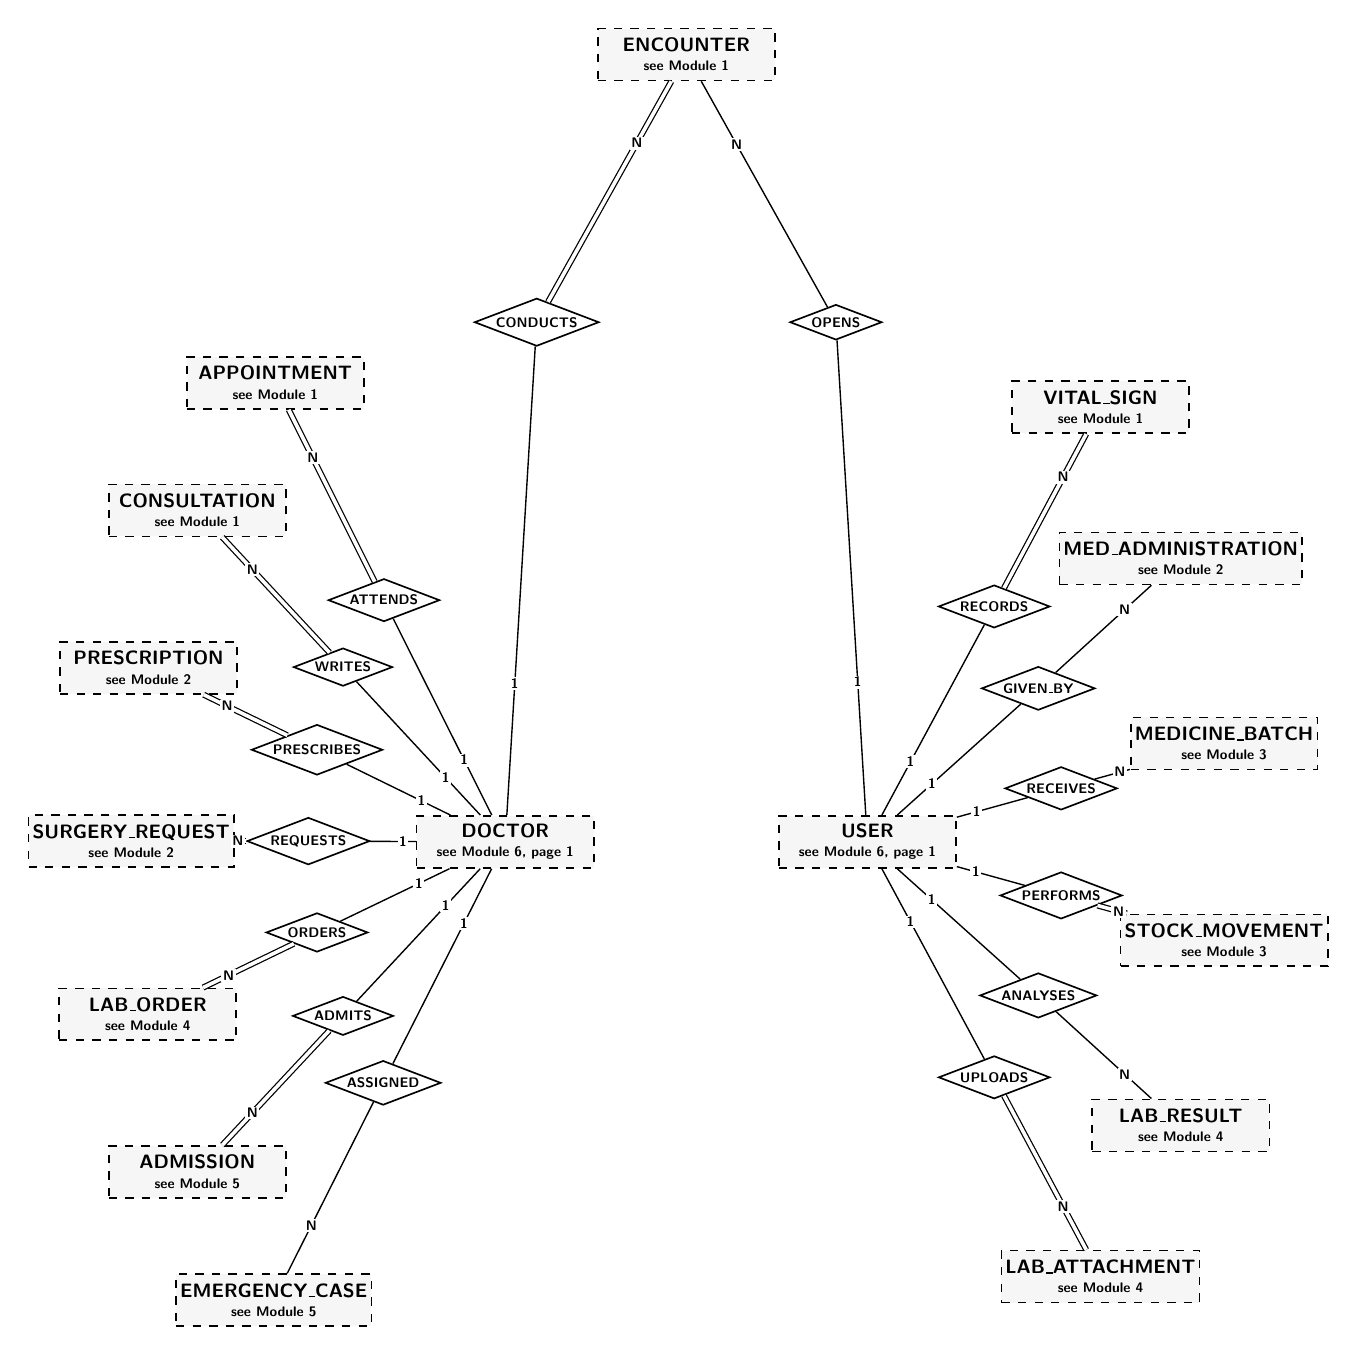
\begin{tikzpicture}[x=1cm,y=1cm]
\node[refent] (DOCTOR) at (6.2,-11.6) {DOCTOR\\[-1pt]{\tiny see Module 6, page 1}};
\node[refent] (USER) at (10.8,-11.6) {USER\\[-1pt]{\tiny see Module 6, page 1}};
\node[refent] (ENCOUNTER) at (8.5,-1.6) {ENCOUNTER\\[-1pt]{\tiny see Module 1}};
\node[refent] (APPOINTMENT) at (3.28,-5.77) {APPOINTMENT\\[-1pt]{\tiny see Module 1}};
\node[refent] (CONSULTATION) at (2.29,-7.39) {CONSULTATION\\[-1pt]{\tiny see Module 1}};
\node[refent] (PRESCRIPTION) at (1.67,-9.39) {PRESCRIPTION\\[-1pt]{\tiny see Module 2}};
\node[refent] (SURGERY_REQUEST) at (1.45,-11.59) {SURGERY\_REQUEST\\[-1pt]{\tiny see Module 2}};
\node[refent] (LAB_ORDER) at (1.66,-13.79) {LAB\_ORDER\\[-1pt]{\tiny see Module 4}};
\node[refent] (ADMISSION) at (2.29,-15.79) {ADMISSION\\[-1pt]{\tiny see Module 5}};
\node[refent] (EMERGENCY_CASE) at (3.26,-17.42) {EMERGENCY\_CASE\\[-1pt]{\tiny see Module 5}};
\node[refent] (VITAL_SIGN) at (13.76,-6.08) {VITAL\_SIGN\\[-1pt]{\tiny see Module 1}};
\node[refent] (MED_ADMINISTRATION) at (14.78,-8) {MED\_ADMINISTRATION\\[-1pt]{\tiny see Module 2}};
\node[refent] (MEDICINE_BATCH) at (15.33,-10.35) {MEDICINE\_BATCH\\[-1pt]{\tiny see Module 3}};
\node[refent] (STOCK_MOVEMENT) at (15.33,-12.85) {STOCK\_MOVEMENT\\[-1pt]{\tiny see Module 3}};
\node[refent] (LAB_RESULT) at (14.78,-15.2) {LAB\_RESULT\\[-1pt]{\tiny see Module 4}};
\node[refent] (LAB_ATTACHMENT) at (13.76,-17.12) {LAB\_ATTACHMENT\\[-1pt]{\tiny see Module 4}};
\node[rel] (ATTENDS) at (4.66,-8.53) {ATTENDS};
\draw[partial] (ATTENDS) -- node[card,pos=0.72] {1} (DOCTOR);
\draw[total] (ATTENDS) -- node[card,pos=0.72] {N} (APPOINTMENT);
\node[rel] (CONDUCTS) at (6.6,-5) {CONDUCTS};
\draw[partial] (CONDUCTS) -- node[card,pos=0.72] {1} (DOCTOR);
\draw[total] (CONDUCTS) -- node[card,pos=0.72] {N} (ENCOUNTER);
\node[rel] (OPENS) at (10.4,-5) {OPENS};
\draw[partial] (OPENS) -- node[card,pos=0.72] {1} (USER);
\draw[partial] (OPENS) -- node[card,pos=0.72] {N} (ENCOUNTER);
\node[rel] (RECORDS) at (12.41,-8.61) {RECORDS};
\draw[partial] (RECORDS) -- node[card,pos=0.72] {1} (USER);
\draw[total] (RECORDS) -- node[card,pos=0.72] {N} (VITAL_SIGN);
\node[rel] (WRITES) at (4.14,-9.38) {WRITES};
\draw[partial] (WRITES) -- node[card,pos=0.72] {1} (DOCTOR);
\draw[total] (WRITES) -- node[card,pos=0.72] {N} (CONSULTATION);
\node[rel] (PRESCRIBES) at (3.81,-10.43) {PRESCRIBES};
\draw[partial] (PRESCRIBES) -- node[card,pos=0.72] {1} (DOCTOR);
\draw[total] (PRESCRIBES) -- node[card,pos=0.72] {N} (PRESCRIPTION);
\node[rel] (GIVEN_BY) at (12.97,-9.65) {GIVEN\_BY};
\draw[partial] (GIVEN_BY) -- node[card,pos=0.72] {1} (USER);
\draw[partial] (GIVEN_BY) -- node[card,pos=0.72] {N} (MED_ADMINISTRATION);
\node[rel] (REQUESTS) at (3.7,-11.59) {REQUESTS};
\draw[partial] (REQUESTS) -- node[card,pos=0.72] {1} (DOCTOR);
\draw[total] (REQUESTS) -- node[card,pos=0.72] {N} (SURGERY_REQUEST);
\node[rel] (RECEIVES) at (13.26,-10.92) {RECEIVES};
\draw[partial] (RECEIVES) -- node[card,pos=0.72] {1} (USER);
\draw[partial] (RECEIVES) -- node[card,pos=0.72] {N} (MEDICINE_BATCH);
\node[rel] (PERFORMS) at (13.26,-12.28) {PERFORMS};
\draw[partial] (PERFORMS) -- node[card,pos=0.72] {1} (USER);
\draw[total] (PERFORMS) -- node[card,pos=0.72] {N} (STOCK_MOVEMENT);
\node[rel] (ORDERS) at (3.81,-12.75) {ORDERS};
\draw[partial] (ORDERS) -- node[card,pos=0.72] {1} (DOCTOR);
\draw[total] (ORDERS) -- node[card,pos=0.72] {N} (LAB_ORDER);
\node[rel] (ANALYSES) at (12.97,-13.55) {ANALYSES};
\draw[partial] (ANALYSES) -- node[card,pos=0.72] {1} (USER);
\draw[partial] (ANALYSES) -- node[card,pos=0.72] {N} (LAB_RESULT);
\node[rel] (UPLOADS) at (12.41,-14.59) {UPLOADS};
\draw[partial] (UPLOADS) -- node[card,pos=0.72] {1} (USER);
\draw[total] (UPLOADS) -- node[card,pos=0.72] {N} (LAB_ATTACHMENT);
\node[rel] (ADMITS) at (4.14,-13.81) {ADMITS};
\draw[partial] (ADMITS) -- node[card,pos=0.72] {1} (DOCTOR);
\draw[total] (ADMITS) -- node[card,pos=0.72] {N} (ADMISSION);
\node[rel] (ASSIGNED) at (4.65,-14.66) {ASSIGNED};
\draw[partial] (ASSIGNED) -- node[card,pos=0.72] {1} (DOCTOR);
\draw[partial] (ASSIGNED) -- node[card,pos=0.72] {N} (EMERGENCY_CASE);
\end{tikzpicture}
\minilegend
\caption{Module 6, Staff and audit (page 2 of 2): the records each doctor and each staff account is linked to}\label{fig:m6b}
\end{figure}

\section{Explanation of the ER Diagram}
\textbf{Reading the diagrams.} A line ends at an entity with the cardinality that entity has in the
relationship. For example, \textsc{books} reads ``one PATIENT books N APPOINTMENTs''. A double line means
every instance of that entity takes part: every appointment is for a patient (\tbl{appointments.patient\_id}
is NOT NULL), while a patient need not have an appointment (single line). Optional links, such as a
prescription written outside a visit, are partial on both sides.

\textbf{Weak entities.} An entity is weak here only when the schema identifies it within its owner, that is,
its natural identifier is unique only together with the owner's key and the owner is mandatory:
\begin{itemize}
\item \textbf{BED} (owner WARD, partial key \dashuline{bed\_number}): bed numbers are unique only within a ward, UNIQUE (\tbl{ward\_id, bed\_number}).
\item \textbf{MEDICINE\_BATCH} (owner MEDICINE, partial key \dashuline{batch\_number}): a supplier's batch number is unique only for one medicine, UNIQUE (\tbl{medicine\_id, batch\_number}).
\item \textbf{DOCTOR\_SCHEDULE} (owner DOCTOR, partial key \dashuline{day\_of\_week}, \dashuline{start\_time}): a slot exists only as a slot of one doctor, UNIQUE (\tbl{doctor\_id, day\_of\_week, start\_time}), deleted with the doctor (ON DELETE CASCADE).
\item \textbf{DAILY\_ANALYTICS} (owner DOCTOR, partial key \dashuline{analytics\_date}): one statistics row per doctor per day, UNIQUE (\tbl{doctor\_id, analytics\_date}), deleted with the doctor.
\end{itemize}
In the tables each also has a surrogate integer key, added during mapping (Section~4.2). Line items such as
BILL\_ITEM are \emph{not} modelled as weak: nothing in the schema identifies them within their bill, so their own
key identifies them.

\textbf{Module 1, Patients and visits} (Figures~\ref{fig:m1a}, \ref{fig:m1b}). PATIENT books APPOINTMENTs and has
ENCOUNTERs (visits). An appointment \textsc{becomes} at most one encounter and an encounter comes from at most one
appointment (1:1, both partial: walk-ins and emergencies have no appointment). VITAL\_SIGN readings and
CONSULTATION notes always name their patient (total) and are filed under a visit (\textsc{taken\_in},
\textsc{note\_in}) or, for inpatients, an admission (\textsc{taken\_on}, \textsc{stay\_note}). A consultation may
also refer to its appointment (\textsc{note\_for}). Attributes show the derived \emph{age} (computed from
\emph{date\_of\_birth}, never stored), the multivalued \emph{allergies}, and the composite \emph{slot},
\emph{timeline} and \emph{blood\_pressure}. Links to other modules: DOCTOR \textsc{attends} appointments,
\textsc{conducts} encounters and \textsc{writes} notes; USER \textsc{opens} an encounter and \textsc{records} vitals
(Module~6); PATIENT is \textsc{admitted}, \textsc{arrives} as an emergency, is \textsc{billed}, and appears in
\textsc{occupies} (Module~5); PATIENT, ENCOUNTER and CONSULTATION are linked to prescriptions and surgery requests
(Module~2) and lab orders (Module~4).

\textbf{Module 2, Clinical orders} (Figure~\ref{fig:m2}). A PRESCRIPTION \textsc{lists} its PRESCRIPTION\_ITEMs
(total on the item side). Each item is \textsc{of\_drug} one MEDICINE and is \textsc{filled\_from} one or more
MEDICINE\_BATCHes (M:N, with the relationship attribute \emph{quantity}). Every MED\_ADMINISTRATION (a dose on the
MAR) is \textsc{given\_as} part of one item (total) and optionally belongs to an admission and to the nurse who
recorded it. A prescription and a SURGERY\_REQUEST each belong to a patient and a doctor (total) and optionally to
the visit, note or admission they were written in.

\textbf{Module 3, Pharmacy} (Figure~\ref{fig:m3}). MEDICINE \textsc{has\_batch} MEDICINE\_BATCHes through an
identifying relationship. Every STOCK\_MOVEMENT \textsc{moves} one medicine (total) and, when it touched a batch,
comes \textsc{from\_batch} it; movements from before batches existed have none (partial). The medicine's
\emph{stock\_quantity} is drawn as derived: it is the sum of its batches, stored for speed and kept equal in the
same transaction (Section~6.6). USER links: \textsc{receives} (batches) and \textsc{performs} (movements).

\textbf{Module 4, Laboratory} (Figure~\ref{fig:m4}). A LAB\_ORDER is \textsc{of\_test} one LAB\_TEST, and
\textsc{yields} at most one LAB\_RESULT (1:1; every result has its order, total). A result has any number of
LAB\_ATTACHMENTs. Orders link to the patient and doctor (total) and optionally to the visit, note and admission;
tests to the DEPARTMENT that \textsc{offers} them; results and files to the USER who \textsc{analyses} and
\textsc{uploads} them.

\textbf{Module 5, Beds and admissions} (Figures~\ref{fig:m5a}, \ref{fig:m5b}). A WARD \textsc{has\_bed} BEDs
(identifying). An ADMISSION is \textsc{allocated} one bed, is \textsc{admitted} for one patient by one doctor
(\textsc{admits}) to one department (\textsc{admitted\_to}), all total. \textsc{occupies} is ternary: each row of
the bed history joins one bed, one admission and its patient, with the attributes \emph{assigned\_at},
\emph{released\_at} and \emph{status}; every admission takes part (total), because a trigger writes the row.
An EMERGENCY\_CASE may be \textsc{carried} by an AMBULANCE, \textsc{assigned} a doctor and \textsc{given\_bed}, and
\textsc{results\_in} an admission; all partial, because cases wait in a queue first. Figure~\ref{fig:m5b} shows the
six records an admission can cover (Modules 1, 2 and 4) and billing: a BILL is \textsc{billed} to one patient
(total), optionally for an admission, and \textsc{itemises} BILL\_ITEMs whose \emph{total\_price} is derived
(quantity $\times$ unit price); the bill's \emph{total\_amount} is the stored sum of its items.

\textbf{Module 6, Staff and audit} (Figures~\ref{fig:m6a}, \ref{fig:m6b}). A USER account \textsc{is\_doctor} for at
most one DOCTOR (1:1; every doctor has an account). A doctor \textsc{works\_in} one DEPARTMENT and has
DOCTOR\_SCHEDULE slots and DAILY\_ANALYTICS rows (both weak). A WARD\_ASSIGNMENT joins a nurse
(\textsc{nurse\_of}, total) to a ward (\textsc{covers}, total) for a period of days, ended early at the moment an
administrator ends it (\emph{ended\_at}), and records the administrator who \textsc{assigns} it. Every AUDIT\_LOG row \textsc{logs} the user who acted, when known (failed logins have none).
Figure~\ref{fig:m6b} gathers, for DOCTOR and USER, every relationship that enters them from Modules~1 to~5, so the
two pages of Module~6 together show all 15 links of these two entities.

\chapter{ER-to-Relational Mapping}

\section{Mapping Rules}
The standard rules were applied, with one project-wide convention: every entity gets a surrogate integer
primary key (\tbl{AUTO\_INCREMENT}), and natural identifiers become UNIQUE keys. Names, phone numbers and batch
numbers are not reliable identifiers, and narrow integer keys keep foreign keys and InnoDB's clustered index small.
\begin{enumerate}
\item \textbf{Strong entity} $\to$ a table with its simple attributes; its key becomes the primary key.
\item \textbf{Weak entity} $\to$ a table holding the owner's key as a foreign key (NOT NULL) plus the partial key; (owner key, partial key) is a UNIQUE key. A surrogate primary key is added.
\item \textbf{1:1} $\to$ the foreign key goes on the side that may be missing, with a UNIQUE constraint.
\item \textbf{1:N} $\to$ the foreign key goes on the N side; NOT NULL when the N side's participation is total.
\item \textbf{M:N and ternary} $\to$ a new table with a foreign key to each participant and the relationship's attributes.
\item \textbf{Composite attribute} $\to$ its components become columns. \textbf{Multivalued attribute} $\to$ a separate table (owner key, value), or (as here, Section~4.2) one column when the value is never searched element by element. \textbf{Derived attribute} $\to$ not stored, or a generated column, or a stored copy kept up to date.
\end{enumerate}

\section{Step-by-Step Conversion}
\begin{tabularx}{\textwidth}{@{}R{3.1cm}Y@{}}
\toprule
\textbf{ER construct} & \textbf{Relation in hospital\_db (real example)} \\\midrule
Strong entity & PATIENT $\to$ \tbl{patients(\underline{patient\_id}, name, date\_of\_birth, gender, \dots, abha\_number)}; ABHA becomes UNIQUE \tbl{uq\_patients\_abha}. Likewise for the 25 other strong entities. \\
Weak entity & BED (owner WARD) $\to$ \tbl{beds(\underline{bed\_id}, ward\_id\textsuperscript{FK}, bed\_number, \dots)} with UNIQUE (\tbl{ward\_id, bed\_number}); MEDICINE\_BATCH $\to$ \tbl{medicine\_batches} with UNIQUE (\tbl{medicine\_id, batch\_number}); DOCTOR\_SCHEDULE and DAILY\_ANALYTICS likewise, with ON DELETE CASCADE from \tbl{doctors}. \\
1:1 & \textsc{becomes}: \tbl{encounters.appointment\_id} (NULL for walk-ins) with UNIQUE \tbl{uq\_encounters\_appointment}; \textsc{is\_doctor}: \tbl{doctors.user\_id} NOT NULL UNIQUE (\tbl{uq\_doctors\_user\_id}); \textsc{yields}: \tbl{lab\_results.order\_id} NOT NULL UNIQUE. \\
1:N & \textsc{books}: \tbl{appointments.patient\_id} NOT NULL (total); \textsc{carries}: \tbl{emergency\_cases.ambulance\_id} NULL (partial). 64 relationships are mapped this way. \\
M:N with attribute & \textsc{filled\_from} $\to$ \tbl{prescription\_item\_batches(\underline{id}, item\_id\textsuperscript{FK}, batch\_id\textsuperscript{FK}, quantity)}, UNIQUE (\tbl{item\_id, batch\_id}). \\
Ternary with attributes & \textsc{occupies} $\to$ \tbl{bed\_assignment\_log(\underline{log\_id}, bed\_id\textsuperscript{FK}, patient\_id\textsuperscript{FK}, admission\_id\textsuperscript{FK}, assigned\_at, released\_at, status)}. \\
Composite & \emph{blood\_pressure} $\to$ \tbl{bp\_systolic, bp\_diastolic} (CHECK: both or neither, systolic > diastolic); \emph{slot} $\to$ \tbl{appointment\_date, appointment\_time}. \\
Multivalued & \emph{allergies} is stored as one text column \tbl{patients.allergies}: the application only displays it on the chart and never queries one allergy, so a separate \tbl{patient\_allergies} table was not created (a limitation, Section~11.2). \\
Derived & \emph{age}: not stored, computed as \tbl{TIMESTAMPDIFF(YEAR, date\_of\_birth, ?)} with today's date in India as the parameter; \emph{total\_price}: generated column \tbl{quantity * unit\_price}; \emph{stock\_quantity}, \emph{total\_amount}, \emph{current\_workload}: stored copies kept equal by transactions and triggers (Section~6.6). \\
\bottomrule
\end{tabularx}

\section{Final Relational Schema}
All 33 relations, with columns in table order. \underline{Underlined}: primary key. \textit{Italic}\textsuperscript{FK}:
foreign key (with its target when the name does not say it). \textsuperscript{G}: generated column. \textsc{uk}: other
candidate keys (UNIQUE). Not shown: the 15 composite consistency keys of Section~6.5, which re-check pairs of
these foreign keys.

\begin{footnotesize}
\relation{patients}{\underline{patient\_id}, name, date\_of\_birth, dob\_estimated, gender, blood\_group, phone, address, emergency\_contact, created\_at, updated\_at, allergies, abha\_number}{(abha\_number)}
\relation{appointments}{\underline{appointment\_id}, \fk{patient\_id}{}, \fk{doctor\_id}{}, appointment\_date, appointment\_time, status, reason, notes, created\_at, updated\_at}{(doctor\_id, appointment\_date, appointment\_time)}
\relation{encounters}{\underline{encounter\_id}, \fk{patient\_id}{}, \fk{doctor\_id}{}, \fk{appointment\_id}{}, \fk{admission\_id}{}, encounter\_type, status, arrived\_at, triaged\_at, start\_timestamp, end\_timestamp, \fk{created\_by}{users}, backfilled\_from, created\_at, updated\_at}{(appointment\_id); (backfilled\_from)}
\relation{consultations}{\underline{consultation\_id}, \fk{appointment\_id}{}, \fk{patient\_id}{}, \fk{doctor\_id}{}, \fk{admission\_id}{}, symptoms, diagnosis, assessment, plan, notes, consultation\_time, created\_at, \fk{encounter\_id}{}}{}
\relation{vital\_signs}{\underline{vital\_id}, \fk{patient\_id}{}, \fk{encounter\_id}{}, \fk{admission\_id}{}, recorded\_at\_utc, \fk{recorded\_by}{users}, temperature\_c, pulse\_bpm, resp\_rate, bp\_systolic, bp\_diastolic, spo2\_pct, pain\_score, notes, created\_at}{}
\relation{surgery\_requests}{\underline{request\_id}, \fk{patient\_id}{}, \fk{doctor\_id}{}, procedure\_name, diagnosis, priority, requested\_date, status, notes, created\_at, updated\_at, \fk{encounter\_id}{}}{}
\relation{departments}{\underline{department\_id}, name, description, floor, phone, is\_active}{(name)}
\relation{wards}{\underline{ward\_id}, name, \fk{department\_id}{}, floor, capacity, ward\_type}{}
\relation{beds}{\underline{bed\_id}, \fk{ward\_id}{}, bed\_number, bed\_type, status, has\_ventilator}{(ward\_id, bed\_number)}
\relation{admissions}{\underline{admission\_id}, \fk{patient\_id}{}, \fk{doctor\_id}{}, \fk{bed\_id}{}, \fk{department\_id}{}, \fk{emergency\_id}{}, admission\_date, discharge\_date, status, diagnosis, notes, created\_at, updated\_at}{}
\relation{bed\_assignment\_log}{\underline{log\_id}, \fk{bed\_id}{}, \fk{patient\_id}{}, \fk{admission\_id}{}, assigned\_at, released\_at, status}{}
\relation{emergency\_cases}{\underline{emergency\_id}, \fk{patient\_id}{}, \fk{ambulance\_id}{}, severity, symptoms, arrival\_time, required\_specialization, required\_bed\_type, ventilator\_required, status, \fk{assigned\_doctor\_id}{doctors}, \fk{assigned\_bed\_id}{beds}, notes, created\_at, updated\_at}{}
\relation{ambulances}{\underline{ambulance\_id}, vehicle\_number, driver\_name, driver\_phone, current\_location, status}{(vehicle\_number)}
\relation{medicines}{\underline{medicine\_id}, name, category, manufacturer, stock\_quantity, reorder\_level, unit\_price, expiry\_date, requires\_prescription, created\_at, updated\_at}{}
\relation{medicine\_batches}{\underline{batch\_id}, \fk{medicine\_id}{}, batch\_number, quantity, expiry\_date, received\_date, \fk{received\_by}{users}, created\_at, updated\_at}{(medicine\_id, batch\_number)}
\relation{prescriptions}{\underline{prescription\_id}, \fk{consultation\_id}{}, \fk{patient\_id}{}, \fk{doctor\_id}{}, prescription\_date, status, notes, created\_at, \fk{encounter\_id}{}, \fk{admission\_id}{}}{}
\relation{prescription\_items}{\underline{item\_id}, \fk{prescription\_id}{}, \fk{medicine\_id}{}, dosage, frequency, duration, quantity, dispensed, dispensed\_at, frequency\_code, duration\_days, route, units\_per\_dose}{}
\relation{prescription\_item\_batches}{\underline{id}, \fk{item\_id}{}, \fk{batch\_id}{}, quantity, created\_at}{(item\_id, batch\_id)}
\relation{pharmacy\_stock\_movements}{\underline{movement\_id}, \fk{medicine\_id}{}, movement\_type, quantity, reason, notes, \fk{performed\_by}{users}, created\_at, reference\_id, \fk{batch\_id}{}}{}
\relation{medication\_administrations}{\underline{administration\_id}, \fk{prescription\_item\_id}{prescription\_items}, \fk{admission\_id}{}, scheduled\_at\_utc, status, administered\_at\_utc, dose\_given, route\_given, reason, \fk{recorded\_by}{users}, recorded\_at\_utc, created\_at, updated\_at}{(prescription\_item\_id, scheduled\_at\_utc)}
\relation{lab\_tests}{\underline{test\_id}, name, category, \fk{department\_id}{}, normal\_range, unit, cost, reference\_low, reference\_high, critical\_low, critical\_high}{}
\relation{lab\_orders}{\underline{order\_id}, \fk{consultation\_id}{}, \fk{patient\_id}{}, \fk{doctor\_id}{}, \fk{test\_id}{}, order\_date, status, priority, notes, created\_at, updated\_at, \fk{encounter\_id}{}, \fk{admission\_id}{}}{}
\relation{lab\_results}{\underline{result\_id}, \fk{order\_id}{}, result\_value, unit, reference\_range, interpretation, result\_date, technician\_notes, \fk{performed\_by}{users}, reviewed\_by\_doctor, reviewed\_at, created\_at, numeric\_value, reference\_low, reference\_high, interpretation\_source}{(order\_id)}
\relation{lab\_result\_attachments}{\underline{attachment\_id}, \fk{result\_id}{}, original\_filename, stored\_filename, mime\_type, file\_size, \fk{uploaded\_by}{users}, uploaded\_at}{(stored\_filename)}
\relation{users}{\underline{user\_id}, username, password\_hash, role, full\_name, email, phone, is\_active, created\_at, updated\_at}{(email); (username)}
\relation{doctors}{\underline{doctor\_id}, \fk{user\_id}{}, \fk{department\_id}{}, name, specialization, phone, status, shift, current\_workload, max\_workload, created\_at, updated\_at}{(user\_id)}
\relation{doctor\_schedules}{\underline{schedule\_id}, \fk{doctor\_id}{}, day\_of\_week, start\_time, end\_time, is\_available}{(doctor\_id, day\_of\_week, start\_time)}
\relation{doctor\_daily\_analytics}{\underline{analytics\_id}, \fk{doctor\_id}{}, analytics\_date, patients\_seen, emergency\_cases, appointment\_patients, patients\_treated, cases\_solved, cases\_postponed, cases\_cancelled, cases\_pending, created\_at, updated\_at}{(doctor\_id, analytics\_date)}
\relation{nurse\_ward\_assignments}{\underline{assignment\_id}, \fk{nurse\_user\_id}{users}, \fk{ward\_id}{}, start\_date, end\_date, \fk{assigned\_by}{users}, created\_at, updated\_at}{}
\relation{bills}{\underline{bill\_id}, \fk{patient\_id}{}, \fk{admission\_id}{}, bill\_date, total\_amount, paid\_amount, status, payment\_method, notes, created\_at, updated\_at}{}
\relation{bill\_items}{\underline{item\_id}, \fk{bill\_id}{}, description, category, quantity, unit\_price, total\_price\gen, created\_at}{}
\relation{audit\_logs}{\underline{audit\_id}, \fk{user\_id}{}, role, action, entity\_type, entity\_id, patient\_id, outcome, status\_code, method, path, ip\_address, details, created\_at}{}
\relation{schema\_migrations}{\underline{version}, applied\_at, note}{}

\end{footnotesize}

\chapter{Functional Dependencies}

\section{Identification of Functional Dependencies}
A functional dependency $X \to Y$ holds when any two rows with the same $X$ have the same $Y$. Each one listed here
comes from a business rule that the schema or the code enforces: a primary or UNIQUE key, a foreign key whose
value is copied from its parent when a row is written, or a computed value. A pattern that merely happens to hold
in today's rows is not listed. For a nullable left side (for example \tbl{encounter\_id}), the dependency applies to
the rows where it is not NULL, as in SQL's treatment of UNIQUE. Examples:
\[ \textit{patient\_id} \to \textit{name, date\_of\_birth, gender, blood\_group, phone, \dots, abha\_number} \]
\[ \textit{doctor\_id, appointment\_date, appointment\_time} \to \textit{appointment\_id} \]
\[ \textit{encounter\_id} \to \textit{patient\_id, doctor\_id} \quad (\text{in } \tbl{lab\_orders}) \]

\section{Candidate Keys and Attribute Classification}
Table~\ref{tab:fds} gives, for every relation, its dependencies, its candidate keys, its prime attributes (those
in some candidate key) and the number of non-prime attributes (all the others). A UNIQUE column that allows NULL
(such as \tbl{abha\_number}) identifies a row only when present; it is listed as a key because MySQL enforces it.

{\scriptsize\setlength{\tabcolsep}{3pt}
\begin{longtable}{@{}R{2.8cm}R{5.8cm}R{3.5cm}R{2.8cm}c@{}}
\caption{Functional dependencies, candidate keys and attribute classification}\label{tab:fds}\\
\toprule
\textbf{Relation} & \textbf{Functional dependencies} & \textbf{Candidate keys} & \textbf{Prime attributes} & \textbf{Non-prime} \\\midrule\endfirsthead
\toprule\textbf{Relation} & \textbf{Functional dependencies} & \textbf{Candidate keys} & \textbf{Prime attributes} & \textbf{Non-prime} \\\midrule\endhead
\rows{generated/fd-table.tex}
\bottomrule
\end{longtable}}

\section{FD Analysis}
\begin{itemize}
\item \textbf{Keys.} Each primary key determines its row. Each UNIQUE key is a business identifier with its own
dependency: a doctor's slot (\tbl{doctor\_id, appointment\_date, appointment\_time}) identifies one appointment,
because a doctor cannot be in two places; a ward and bed number identify one bed; a medicine and supplier batch
number identify one batch; an order identifies its single result.
\item \textbf{Copied context.} \tbl{lab\_orders}, \tbl{prescriptions}, \tbl{consultations}, \tbl{surgery\_requests}
and \tbl{vital\_signs} store the patient (and doctor) of the visit, admission or note they are filed under. The
code copies these from the parent and checks them (\tbl{resolveEncounterForRecord}, \tbl{resolveOrderContext}),
and composite foreign keys now enforce them, so \tbl{encounter\_id} $\to$ \tbl{patient\_id, doctor\_id} is a real
dependency in those tables. In \tbl{pharmacy\_stock\_movements}, \tbl{batch\_id} $\to$ \tbl{medicine\_id} for the same reason.
\item \textbf{Flags.} In \tbl{prescription\_items} the single dispensing statement sets
\tbl{dispensed\_at = NOW()} and \tbl{dispensed = TRUE} together, so \tbl{dispensed\_at} $\to$ \tbl{dispensed}.
\item \textbf{Removed by normalization.} Three dependencies held in the schema before this work and were removed
by decomposition (Chapter~6): \tbl{ward\_id} $\to$ \tbl{floor} in \tbl{beds}, \tbl{doctor\_id} $\to$
\tbl{department\_id} in \tbl{appointments}, \tbl{prescription\_item\_id} $\to$ \tbl{patient\_id} in
\tbl{medication\_administrations}; a fourth, (\tbl{quantity, unit\_price}) $\to$ \tbl{total\_price} in
\tbl{bill\_items}, now holds by definition of a generated column.
\item \textbf{Not dependencies.} Some patterns look like dependencies but are not rules, so they are not listed:
\tbl{wards.department\_id} $\not\to$ \tbl{floor} (a department may span floors; each ward's floor is entered);
\tbl{admissions.bed\_id} $\not\to$ \tbl{department\_id} (staff choose the department on the form);
\tbl{emergency\_cases.required\_bed\_type} $\not\to$ \tbl{ventilator\_required} (an ICU case may or may not need one);
\tbl{audit\_logs.user\_id} $\not\to$ \tbl{role} (a seed migration logs the role MIGRATION); and the order's admission
is a snapshot taken when the order was placed, not a function of its visit.
\end{itemize}

\chapter{Database Normalization}
Normalization is shown in two parts. Sections~6.1 to 6.5 take one outpatient record, as a clerk might keep it on
paper, through each normal form to the tables this system has. The patient, doctor, department, medicines and tests
in it are real rows of the seed data; the visit itself is illustrative. The same sections then show the
four decompositions performed on the live schema (migrations 015--022) at the normal form each one fixed.
Section~6.6 gives the final schema and the normal form of all 33 tables.

\section{Unnormalized Form (UNF)}
\begin{table}[H]\centering\scriptsize\setlength{\tabcolsep}{3pt}
\caption{One outpatient visit as a single unnormalized record}\label{tab:unf}
\begin{tabular}{@{}p{2.1cm}p{1.5cm}p{2.0cm}p{1.6cm}p{2.3cm}p{3.1cm}p{3.3cm}@{}}
\toprule
\textbf{Patient} & \textbf{Phone} & \textbf{Doctor} & \textbf{Dept} & \textbf{Visit} & \textbf{Medicines (dose, freq, qty)} & \textbf{Tests (cost, result)} \\\midrule
Aarav Sharma, M, 1985-03-15 & 9111000001 & Dr. John Smith & Cardiology, floor 2 & 2026-10-13 09:30; chest tightness / suspected angina & Aspirin 75mg (75 mg, OD, 30); Atorvastatin 10mg (10 mg, OD, 30) & Lipid Profile (800.00, pending); Blood Glucose Fasting (150.00, 128 mg/dL, HIGH) \\
\bottomrule
\end{tabular}
\end{table}
\textbf{Problems.} \emph{Medicines} and \emph{Tests} are repeating groups (a list in one cell), \emph{Patient},
\emph{Dept} and \emph{Visit} each pack several facts into one cell, and there is no key.

\section{First Normal Form (1NF)}
Each cell is split into atomic values and each repeated item into its own row. The record becomes one row per
(medicine, test) pair of the visit, four rows in all:
\begin{center}\scriptsize
VISIT\_RECORD(\underline{patient\_name, visit\_time, medicine, test}, dob, gender, phone, doctor, department, dept\_floor,
symptoms, diagnosis, dose, frequency, quantity, test\_cost, result\_value, interpretation)
\end{center}
It is in 1NF but every patient and visit fact is repeated four times, giving the three anomalies:
\textbf{update} (a new phone number must be written in four rows), \textbf{insertion} (a test cannot be recorded
for a visit without a medicine) and \textbf{deletion} (removing the last medicine loses the diagnosis).
Every live table is in 1NF: all columns are single-valued and typed, and lists such as a prescription's lines
are rows of their own table.

\section{Second Normal Form (2NF)}
\textbf{The record.} Partial dependencies on the key (\emph{patient, visit time, medicine, test}):
\emph{patient} $\to$ dob, gender, phone; (\emph{patient, visit time}) $\to$ doctor, department, dept\_floor,
symptoms, diagnosis; (\emph{visit, medicine}) $\to$ dose, frequency, quantity; (\emph{visit, test}) $\to$ result;
\emph{test} $\to$ cost. Removing them gives:
\begin{center}\scriptsize
PATIENT(\underline{patient}, dob, gender, phone) \quad VISIT(\underline{patient, visit\_time}, doctor, department, dept\_floor, symptoms, diagnosis)\\
VISIT\_MEDICINE(\underline{patient, visit\_time, medicine}, dose, frequency, quantity) \quad VISIT\_TEST(\underline{patient, visit\_time, test}, result) \quad TEST(\underline{test}, cost)
\end{center}
A surrogate key is then given to each entity (\tbl{patient\_id}, \tbl{encounter\_id}, \dots) because names are not unique.

\textbf{The live schema: three 2NF violations decomposed.} Each was a non-key column depending on part of a
composite candidate key. In each case the determinant's own table already held the value, so the decomposition
removes the copy and reads it through the existing foreign key; no new table was needed.
\begin{enumerate}[before=\small]
\item \textbf{A1, \tbl{beds}.} Key (\tbl{ward\_id, bed\_number}); \tbl{ward\_id} $\to$ \tbl{floor}.
\\ \tbl{beds(\underline{bed\_id}, ward\_id, bed\_number, \sout{floor}, bed\_type, status, has\_ventilator)} $\Rightarrow$
\tbl{beds(\underline{bed\_id}, ward\_id, bed\_number, bed\_type, status, has\_ventilator)} $\bowtie$ \tbl{wards(\underline{ward\_id}, \dots, floor)}.
\item \textbf{A2, \tbl{appointments}.} Key (\tbl{doctor\_id, appointment\_date, appointment\_time}); \tbl{doctor\_id} $\to$ \tbl{department\_id}
(copied from the booked doctor). $\Rightarrow$ \tbl{appointments} without \tbl{department\_id} $\bowtie$ \tbl{doctors(\underline{doctor\_id}, department\_id)};
the view \tbl{v\_appointments} returns the old columns. Four seed rows booked under another department were first set to their doctor's department (old values kept in the audit log).
\item \textbf{A3, \tbl{medication\_administrations}.} Key (\tbl{prescription\_item\_id, scheduled\_at\_utc}); \tbl{prescription\_item\_id} $\to$ \tbl{patient\_id}.
$\Rightarrow$ the dose table without \tbl{patient\_id} $\bowtie$ \tbl{prescription\_items} $\bowtie$ \tbl{prescriptions(\underline{prescription\_id}, patient\_id)}.
\end{enumerate}
Each decomposition is \textbf{lossless}, because the shared attribute is the key of the other relation and every
row was checked to rebuild from the join before the column was dropped (35/35 beds, 9/9 appointments, 15/15 doses).
It is also \textbf{dependency-preserving}, because the removed dependency is now enforced by the other relation's key.

\section{Third Normal Form (3NF)}
\textbf{The record.} In VISIT, department and dept\_floor depend on the doctor, not the visit
(\emph{visit} $\to$ \emph{doctor} $\to$ \emph{department} $\to$ \emph{floor}). Removing the transitive dependencies:
\begin{center}\scriptsize
VISIT(\underline{visit}, patient, doctor, visit\_time, symptoms, diagnosis) \quad DOCTOR(\underline{doctor}, name, department) \quad DEPARTMENT(\underline{department}, name, floor)
\end{center}
A visit can have several notes written by its doctor, so symptoms and diagnosis move to a note of the visit
(\tbl{consultations}); medicines become a catalogue (\tbl{medicines}) and what is prescribed is grouped under a
prescription header.

\textbf{The live schema: one 3NF violation decomposed.} \textbf{A5, \tbl{bill\_items}}:
(\tbl{quantity, unit\_price}) $\to$ \tbl{total\_price}, a dependency through two non-key columns. The column became
\tbl{total\_price DECIMAL(10,2) GENERATED ALWAYS AS (quantity * unit\_price) VIRTUAL}: it is computed when read,
so it cannot disagree, and the API still returns it (19/19 existing rows already matched).

\section{Boyce--Codd Normal Form (BCNF)}
\textbf{The record.} After 3NF every determinant of the record's relations is a key: a prescription line
(\emph{prescription, medicine}) gets its own id, a lab result is determined by its order, and a test's cost by the
test. The result is the tables of this system: PATIENT $\to$ \tbl{patients}; DOCTOR, DEPARTMENT $\to$
\tbl{doctors}, \tbl{departments}; VISIT $\to$ \tbl{appointments} (the booking) and \tbl{encounters} (the visit);
note $\to$ \tbl{consultations}; VISIT\_MEDICINE $\to$ \tbl{prescriptions} + \tbl{prescription\_items}; TEST,
VISIT\_TEST $\to$ \tbl{lab\_tests}, \tbl{lab\_orders} + \tbl{lab\_results}.

\textbf{The live schema: tables checked against BCNF.} 24 of the 33 tables are in BCNF: every non-trivial
dependency has a candidate key on its left (Table~\ref{tab:fds}). Nine are not, and are kept on purpose:
\begin{itemize}
\item \textbf{Eight copy a patient, doctor or medicine from an optional parent} (Table~\ref{tab:kept}), e.g.
\tbl{lab\_orders}: \tbl{encounter\_id} $\to$ \tbl{patient\_id, doctor\_id}. The textbook decomposition (drop
\tbl{patient\_id}, read it through \tbl{encounter\_id}) is \emph{lossy} here: the link is optional, and an order
with no visit would lose its patient (3 of the 9 live orders have neither a visit nor an admission). The
doctor's access check also filters on these columns in every table. So the copies stay, and \textbf{the database
enforces them}: each parent got a UNIQUE key over its id and the copied columns (e.g. \tbl{encounters
(encounter\_id, patient\_id, doctor\_id)}) and each child a composite foreign key to it (\tbl{fk\_ctx\_*}, 15 in all,
migration 018). InnoDB checks a composite foreign key only when none of its columns is NULL, so rows without the
link are unaffected; a copy that disagrees is refused (test T10, Chapter~10).
\item \textbf{\tbl{prescription\_items}}: \tbl{dispensed\_at} $\to$ \tbl{dispensed}. Replacing the flag by
``\tbl{dispensed\_at IS NOT NULL}'' would lose information: three seed items are dispensed with no recorded time,
and the guard against dispensing twice keys on the flag. The dependency is enforced by
\tbl{CHECK (dispensed\_at IS NULL OR dispensed = 1)} (migration 023).
\end{itemize}

\section{Final Normalized Schema}
The final relations are those of Section~4.3. Table~\ref{tab:nf} gives each table's highest normal form before
this work (migration 014) and now; Table~\ref{tab:kept} lists the nine tables outside BCNF and what keeps their
copies consistent. In summary: 20 tables were in BCNF before and 24 are now, every table is in 2NF (the three
2NF violations were decomposed), and the nine remaining are in 2NF with each dependency enforced by the database.

{\scriptsize
\begin{longtable}{@{}lllR{2.3cm}@{\hspace{4mm}}lllR{2.3cm}@{}}
\caption{Normal form of every table, before (migration 014) and now}\label{tab:nf}\\
\toprule
\textbf{Table} & \textbf{Before} & \textbf{Now} & \textbf{Note} & \textbf{Table} & \textbf{Before} & \textbf{Now} & \textbf{Note} \\\midrule\endfirsthead
\toprule\textbf{Table} & \textbf{Before} & \textbf{Now} & \textbf{Note} & \textbf{Table} & \textbf{Before} & \textbf{Now} & \textbf{Note} \\\midrule\endhead
\rows{generated/nf-summary.tex}
\bottomrule
\end{longtable}}

{\scriptsize
\begin{longtable}{@{}R{3.2cm}R{5.0cm}R{8.6cm}@{}}
\caption{The nine tables kept outside BCNF: dependency and how consistency is enforced}\label{tab:kept}\\
\toprule
\textbf{Table} & \textbf{Dependency (left side not a key)} & \textbf{Enforced by} \\\midrule\endfirsthead
\toprule\textbf{Table} & \textbf{Dependency} & \textbf{Enforced by} \\\midrule\endhead
\rows{generated/nf-kept.tex}
\bottomrule
\end{longtable}}

Values derived from \emph{other} tables do not break BCNF inside a table, but they are redundancy, and each is kept
equal by the database: \tbl{medicines.stock\_quantity} (sum of its batches, updated in the dispensing and stock
transactions), \tbl{bills.total\_amount} (sum of its items), \tbl{doctors.current\_workload} and \tbl{beds.status}
(maintained by the admission triggers), and \tbl{appointments.status} (mirrors its visit, written in the same
transaction).

\chapter{Relational Integrity and Constraints}
The schema declares 33 primary keys, 87 foreign keys (72 relationships and 15 composite consistency keys),
23 UNIQUE keys and 31 CHECK constraints, and runs in strict SQL mode, so an invalid value is an error rather than
a silent conversion. Seven triggers keep derived values and the audit log correct. Table~\ref{tab:constraints}
gives a real example of each kind.

{\small
\begin{longtable}{@{}R{2.4cm}R{7.4cm}R{7.0cm}@{}}
\caption{Integrity constraints in hospital\_db, with real examples}\label{tab:constraints}\\
\toprule
\textbf{Constraint} & \textbf{Example} & \textbf{What it prevents} \\\midrule\endfirsthead
\toprule\textbf{Constraint} & \textbf{Example} & \textbf{What it prevents} \\\midrule\endhead
Domain & \tbl{patients.gender ENUM('MALE','FEMALE','OTHER')}; \tbl{bills.total\_amount DECIMAL(12,2)}; \tbl{appointment\_date DATE} & Values outside the column's type or list (``M'', ``tomorrow'') \\
Primary key & \tbl{patients(patient\_id)}; every table has one & Duplicate or missing row identity \\
Foreign key & \tbl{lab\_orders.test\_id} $\to$ \tbl{lab\_tests(test\_id)} & An order for a test that does not exist (test T3) \\
Composite FK & \tbl{lab\_orders(encounter\_id, patient\_id, doctor\_id)} $\to$ \tbl{encounters(encounter\_id, patient\_id, doctor\_id)} & An order whose patient differs from its visit's patient (Section~6.5) \\
UNIQUE & \tbl{users.username}; \tbl{uq\_patients\_abha}; (\tbl{doctor\_id, appointment\_date, appointment\_time}) & Two accounts with one username (T2); one ABHA number for two patients (T6); a double booking (T13) \\
NOT NULL & \tbl{appointments.patient\_id}; \tbl{admissions.bed\_id}; \tbl{lab\_results.order\_id} & An appointment for nobody; an admission without a bed (total participation, Chapter~3) \\
CHECK & \tbl{medicines\_chk\_1 (stock\_quantity >= 0)}; \tbl{bills\_chk\_2 (paid\_amount <= total\_amount)}; \tbl{chk\_vitals\_spo2 (spo2\_pct BETWEEN 50 AND 100)}; \tbl{chk\_patients\_abha\_format} (14 digits) & Negative stock (T4), over-payment, impossible readings, malformed ABHA \\
Generated column & \tbl{bill\_items.total\_price AS (quantity * unit\_price)} & A line total that disagrees with its quantity and price \\
Trigger & \tbl{before\_medicine\_stock\_update} (SIGNAL if negative); \tbl{audit\_logs\_no\_update}, \tbl{audit\_logs\_no\_delete} & Negative stock by any path; editing or deleting audit rows (T12) \\
\bottomrule
\end{longtable}}

\textbf{Referential actions.} Every ON UPDATE rule is NO ACTION (InnoDB treats it as RESTRICT): primary keys are
surrogates and never change. The ON DELETE rule of each foreign key follows the meaning of the relationship:
\begin{itemize}
\item \textbf{RESTRICT (67 keys)} for records that must not lose their parent: a patient with admissions, visits or
bills cannot be deleted (\tbl{DELETE FROM patients WHERE patient\_id = 1} fails with error 1451, Section~8.4).
The application has no delete operation for patients, and staff accounts are deactivated (\tbl{users.is\_active}), never deleted.
\item \textbf{CASCADE (12)} for parts that have no meaning without their whole: \tbl{bill\_items} with their
\tbl{bills}, \tbl{prescription\_items} with their \tbl{prescriptions}, \tbl{lab\_results} with their
\tbl{lab\_orders}, \tbl{doctor\_schedules} and \tbl{doctor\_daily\_analytics} with their doctor (the weak entities).
\item \textbf{SET NULL (8)} for optional references whose loss leaves the child valid: an emergency case keeps its
record when its ambulance (\tbl{ambulance\_id}), doctor or bed is removed; a lab result keeps its value when the
technician's account is removed (\tbl{performed\_by}).
\end{itemize}
Together these keep the data consistent without relying on the application: a row cannot reference a missing row,
a copy cannot disagree with its source, totals cannot go out of range, and the history in the audit log cannot be
rewritten.

\chapter{MySQL Database Implementation}
All outputs in this chapter are real: they were produced on \tbl{hospital\_db\_test}, a database built from the seed
data and every migration (same schema as \tbl{hospital\_db}, checked by a schema-diff script). Statements that change
data were run inside a transaction that was then rolled back.

\section{Database Creation}
The schema is built by numbered migration files (\path{database/migrations/000} to \path{023}), applied in order by
\path{server/scripts/migrate.js}, which backs up the database first and records each file in
\tbl{schema\_migrations}. The database and the restricted account the application runs as:
\begin{lstlisting}[caption={Creating the database and the application's restricted account}]
CREATE DATABASE hospital_db CHARACTER SET utf8mb4 COLLATE utf8mb4_0900_ai_ci;
CREATE USER 'hospital_app'@'127.0.0.1' IDENTIFIED BY RANDOM PASSWORD;
GRANT SELECT, INSERT, UPDATE, DELETE, EXECUTE ON `hospital_db`.* TO 'hospital_app'@'127.0.0.1';
\end{lstlisting}
The application account cannot create, alter or drop tables or triggers; migrations use a separate administrative account.

\section{Table Creation}
Six key tables are shown below, exactly as MySQL reports them (\tbl{SHOW CREATE TABLE}); all 33 are in the complete
script (Appendix~A).

\lstinputlisting[caption={\tbl{patients}: unique ABHA number with a format CHECK}]{generated/create-patients.sql}
\lstinputlisting[caption={\tbl{encounters}: the visit, with its 1:1 link to an appointment and the parent key used by consistency keys}]{generated/create-encounters.sql}
\lstinputlisting[caption={\tbl{admissions}: five foreign keys with RESTRICT, SET NULL and a composite parent key}]{generated/create-admissions.sql}
\lstinputlisting[caption={\tbl{prescription\_items}: structured dosing and the dispensed CHECK}]{generated/create-prescription_items.sql}
\lstinputlisting[caption={\tbl{medicine\_batches}: a weak entity (UNIQUE owner + batch number)}]{generated/create-medicine_batches.sql}
\lstinputlisting[caption={\tbl{bill\_items}: the generated total and CASCADE from its bill}]{generated/create-bill_items.sql}

\section{Data Insertion}
\begin{lstlisting}[caption={Inserting a patient and a bill line (results below)}]
INSERT INTO patients (name, date_of_birth, gender, blood_group, phone, abha_number)
VALUES ('Meera Iyer', '1992-07-14', 'FEMALE', 'B+', '9810012345', '12345678901234');
INSERT INTO bill_items (bill_id, description, category, quantity, unit_price)
VALUES (1, 'Dressing change', 'PROCEDURE', 3, 150.00);
\end{lstlisting}
\textbf{Result:} 1 row each. The patient got \tbl{patient\_id = 37}. The bill line got \tbl{total\_price = 450.00}
without the statement supplying it (generated column). The seed data (\tbl{database/seed.sql}) inserts 17 staff
accounts, 12 doctors, 9 departments, 6 wards, 35 beds, 32 patients, 22 medicines, 15 lab tests and their activity.

\section{Data Modification and Deletion}
\begin{lstlisting}[caption={UPDATE and DELETE, including a cascade and a refused delete (results below)}]
UPDATE bill_items SET quantity = 4 WHERE item_id = 20;
UPDATE beds SET status = 'MAINTENANCE' WHERE bed_id = 1 AND status = 'AVAILABLE';
DELETE FROM bills WHERE bill_id = 1;          -- its bill_items go with it (ON DELETE CASCADE)
DELETE FROM patients WHERE patient_id = 1;    -- refused: the patient is referenced (RESTRICT)
\end{lstlisting}
\textbf{Results:} the bill line's total became 600.00 (4 $\times$ 150.00); bed GEN-A01 became MAINTENANCE (1 row);
deleting bill 1 removed 1 bill and its 8 items (8 $\to$ 0); deleting patient 1 failed with
\tbl{ER\_ROW\_IS\_REFERENCED\_2 (1451)}: foreign key \tbl{bed\_assignment\_log\_ibfk\_2} (\tbl{ON DELETE RESTRICT}).

\section{Sample Database Contents}
\begin{table}[H]\centering
\caption{Sample contents of \tbl{patients}, \tbl{departments} and beds per ward (\tbl{SELECT} on the test database)}\label{tab:sample}
{\scriptsize\setlength{\tabcolsep}{3pt}\begin{tabular}{lllll}\toprule
\textbf{patient\_id} & \textbf{name} & \textbf{date\_of\_birth} & \textbf{gender} & \textbf{blood\_group} \\\midrule
1 & Aarav Sharma & 1985-03-15 & MALE & O+ \\
2 & Diya Patel & 1990-07-22 & FEMALE & A+ \\
3 & Vihaan Reddy & 1978-11-30 & MALE & B+ \\
4 & Ananya Gupta & 1995-05-10 & FEMALE & AB+ \\
5 & Aditya Kumar & 1960-01-20 & MALE & O- \\
\bottomrule\end{tabular}}
\hfill{\scriptsize\setlength{\tabcolsep}{3pt}\begin{tabular}{lll}\toprule
\textbf{department\_id} & \textbf{name} & \textbf{floor} \\\midrule
1 & Emergency & 1 \\
2 & Cardiology & 2 \\
3 & Neurology & 3 \\
4 & Orthopedics & 2 \\
5 & General Medicine & 1 \\
6 & Pediatrics & 1 \\
\bottomrule\end{tabular}}
\hfill{\scriptsize\setlength{\tabcolsep}{3pt}\begin{tabular}{lll}\toprule
\textbf{ward} & \textbf{beds} & \textbf{available} \\\midrule
General Ward A & 10 & 8 \\
General Ward B & 8 & 7 \\
Cardiac Ward & 4 & 2 \\
Pediatric Ward & 3 & 2 \\
ICU Ward & 6 & 2 \\
Emergency Observation & 4 & 3 \\
\bottomrule\end{tabular}}

\end{table}

\section{SQL Query Implementation}
The fifteen queries below cover the ten required kinds, and most are the queries the application itself runs or
reports on. Each gives its SQL, purpose and real output.
\query{1}{Simple SELECT with conditions}{Medicines whose stock has fallen to or below their reorder level (the low-stock alert).}{q1}
\query{2}{ORDER BY}{Available ICU and ventilator beds, ordered by ward and bed number (what the emergency desk looks at first).}{q2}
\query{3}{Aggregates: COUNT, SUM, AVG, MIN, MAX}{Billing summary: how many bills, how much billed and paid, and the smallest, average and largest bill.}{q3}
\query{4}{GROUP BY with HAVING}{Departments that have more than one doctor, with their doctor count and combined capacity.}{q4}
\query{5}{INNER JOIN}{Today's appointments with patient and doctor names; the department comes from the doctor through the view v\_appointments.}{q5}
\query{6}{LEFT JOIN}{Every doctor with the number of ACTIVE admissions they hold, including doctors with none (LEFT JOIN keeps them, COUNT gives 0).}{q6}
\query{7}{Self join (another join type)}{Pairs of doctors who share a specialization: the doctors table joined to itself.}{q7}
\query{8}{Nested query (subquery in WHERE)}{Medicines priced above the average price of all medicines.}{q8}
\query{9}{Correlated subquery}{Each admitted patient with the time of their latest vital-signs reading (NULL: not taken yet). The subquery runs once per admission.}{q9}
\query{10}{IN and EXISTS}{Patients with an ACTIVE admission (EXISTS) who also have a lab order that is not yet completed (IN).}{q10}
\query{11}{ALL and ANY}{Medicines dearer than every antibiotic (> ALL), and antacids dearer than at least one antiplatelet (> ANY).}{q11}
\query{12}{Multiple tables (five-table join)}{Current inpatients with ward, bed, admitting doctor and department.}{q12}
\query{13}{Business question: bed occupancy}{Occupancy by bed type: how full is the hospital? (CASE inside SUM.)}{q13}
\query{14}{Business question: stock that expires soonest}{For each medicine with stock, its usable quantity and next expiry, from the batches (view v\_current\_stock).}{q14}
\query{15}{View}{The view current\_admissions\_view joins admissions with patients, doctors, beds, wards and departments; callers select from it like a table.}{q15}


\section{Advanced DBMS Features}
\textbf{Views (10).} \tbl{v\_appointments} returns appointments with the department taken from the doctor
(Section~6.3), so reads keep their columns after the decomposition; \tbl{v\_current\_stock} shows each medicine's
total, usable and expired quantities and next expiry from its batches (Query~14); \tbl{current\_admissions\_view}
(Query~15), \tbl{available\_beds\_view}, \tbl{bed\_status\_summary\_view}, \tbl{hospital\_occupancy\_view},
\tbl{available\_doctors\_view}, \tbl{doctor\_workload\_view}, \tbl{emergency\_queue\_view} and
\tbl{pending\_bills\_view} give reporting summaries.

\textbf{Triggers (7).} \tbl{after\_admission\_insert} (Listing~\ref{lst:trigger}) and \tbl{after\_admission\_discharge}
keep beds, doctor workload and the bed history in step with admissions;
\tbl{after\_prescription\_dispense} takes a dispensed quantity off \tbl{medicines.stock\_quantity};
\tbl{before\_medicine\_stock\_update} refuses a negative total; \tbl{audit\_logs\_no\_update} and
\tbl{audit\_logs\_no\_delete} make the audit log append-only; \tbl{after\_bed\_assignment\_log} is an empty
placeholder from the original schema.
\lstinputlisting[caption={Trigger \tbl{after\_admission\_insert} (since migration 020, workload counts only ACTIVE admissions)},label={lst:trigger}]{generated/trigger-admission.sql}

\textbf{Stored procedures (5)}, from the original schema: \tbl{sp\_admit\_patient}, \tbl{sp\_discharge\_patient},
\tbl{sp\_allocate\_emergency}, \tbl{sp\_generate\_bill} and \tbl{sp\_get\_emergency\_queue}.

\textbf{Transactions and locking.} Every change runs in a transaction (\tbl{withTransaction} in
\tbl{server/utils/audit.js}): the change and its audit row commit together or not at all. InnoDB runs at REPEATABLE
READ, and operations that read a value and then change it lock the rows first (\tbl{SELECT \dots{} FOR UPDATE}).
To prevent deadlocks, rows are always locked in the same order. Dispensing, for example, locks the prescription,
then its medicines in ascending id, then each medicine's batches by expiry date:
\begin{lstlisting}[caption={Lock order in one dispensing transaction (\tbl{dispenseService})}]
START TRANSACTION;
SELECT status, patient_id FROM prescriptions WHERE prescription_id = ? FOR UPDATE;
SELECT medicine_id, stock_quantity FROM medicines WHERE medicine_id = ? FOR UPDATE;  -- each, ascending id
SELECT batch_id, quantity, expiry_date FROM medicine_batches
WHERE medicine_id = ? AND quantity > 0 AND expiry_date >= CURDATE()
ORDER BY expiry_date, batch_id FOR UPDATE;                                          -- first expiry first out
UPDATE prescription_items SET dispensed = TRUE, dispensed_at = NOW()
WHERE item_id IN (?) AND dispensed = FALSE;              -- trigger after_prescription_dispense lowers the total
UPDATE medicine_batches SET quantity = quantity - ? WHERE batch_id = ?;                -- each batch taken
INSERT INTO prescription_item_batches (item_id, batch_id, quantity) VALUES (?, ?, ?);
INSERT INTO pharmacy_stock_movements (medicine_id, movement_type, quantity, reason, reference_id, performed_by, batch_id)
VALUES (?, 'DISPENSE', ?, 'Dispense Prescription', ?, ?, ?);
UPDATE prescriptions SET status = 'DISPENSED' WHERE prescription_id = ?;
COMMIT;
\end{lstlisting}
The stress test runs 300 rounds of competing prescribing and dispensing on the same two medicines in opposite
orders, and 300 rounds of mixed writers: 0 deadlocks, and every medicine's total equals the sum of its batches.
Bed allocation locks the chosen bed and then the doctor (\tbl{FOR UPDATE}), so two clerks cannot give the same
last ICU bed to two patients.

\chapter{Application Development}

\section{System Architecture}
\begin{figure}[H]\centering
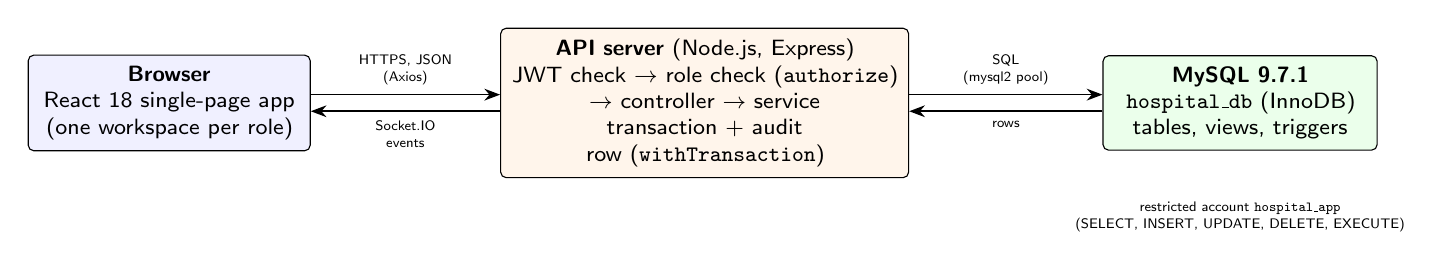
\begin{tikzpicture}[x=1cm,y=1cm, box/.style={draw, rounded corners=2pt, align=center, font=\sffamily\footnotesize, inner sep=4pt, fill=#1}, box/.default=white, arr/.style={-{Stealth[length=2mm]}, line width=0.6pt}]
  \node[box=blue!6, text width=3.3cm] (ui) at (-0.2,0) {\textbf{Browser}\\React 18 single-page app\\(one workspace per role)};
  \node[box=orange!8, text width=4.9cm] (api) at (6.6,0) {\textbf{API server} (Node.js, Express)\\JWT check $\to$ role check (\texttt{authorize})\\$\to$ controller $\to$ service\\transaction + audit row (\texttt{withTransaction})};
  \node[box=green!8, text width=3.2cm] (db) at (13.4,0) {\textbf{MySQL 9.7.1}\\\texttt{hospital\_db} (InnoDB)\\tables, views, triggers};
  \draw[arr] ([yshift=3pt]ui.east) -- node[above, font=\sffamily\tiny, align=center] {HTTPS, JSON\\(Axios)} ([yshift=3pt]api.west);
  \draw[arr] ([yshift=-3pt]api.west) -- node[below, font=\sffamily\tiny, align=center] {Socket.IO\\events} ([yshift=-3pt]ui.east);
  \draw[arr] ([yshift=3pt]api.east) -- node[above, font=\sffamily\tiny, align=center] {SQL\\(mysql2 pool)} ([yshift=3pt]db.west);
  \draw[arr] ([yshift=-3pt]db.west) -- node[below, font=\sffamily\tiny] {rows} ([yshift=-3pt]api.east);
  \node[font=\sffamily\tiny, align=center] at (13.4,-1.45) {restricted account \texttt{hospital\_app}\\(SELECT, INSERT, UPDATE, DELETE, EXECUTE)};
\end{tikzpicture}
\caption{Architecture: three tiers; the database is reached only through the API's restricted account}\label{fig:arch}
\end{figure}

\section{Front-End Technologies}
JavaScript throughout. The client is React 18 with React Router 6 (role-guarded routes), built with Vite 4, calling
the API through Axios and receiving live updates (bed changes, the doctor's queue, the emergency queue) over the
Socket.IO client. The API is Express 4 on Node.js with \texttt{mysql2/promise}, \texttt{jsonwebtoken} (sign-in
tokens), \texttt{bcryptjs} (password hashes) and Multer (lab report uploads). Tests use \texttt{node:test} and Puppeteer.

\section{Application Modules}
The API has 24 routers under \texttt{/api}. They map to the ER modules:
\begin{itemize}
\item \textbf{Patients and visits:} registration and search, appointments, the visit state machine (arrive, triage, start, finish), vital signs, consultation notes.
\item \textbf{Clinical orders:} prescriptions with structured dosing, surgery requests; the nurse's MAR (doses due, given, refused, missed).
\item \textbf{Pharmacy:} the dispense queue, dispensing by batch, stock receipt and adjustment, low-stock and expiry views.
\item \textbf{Laboratory:} the order board, results with automatic flagging, report uploads and secure downloads.
\item \textbf{Beds and admissions:} the bed board, admission and discharge, emergency queue and allocation, ambulances, billing.
\item \textbf{Staff and audit:} staff accounts, nurse ward assignments, doctor dashboard statistics, the audit log viewer.
\end{itemize}

\section{Database Connectivity}
\begin{itemize}
\item \textbf{Pool:} \texttt{server/config/db.js} creates a \texttt{mysql2} connection pool (20 connections) from
\texttt{server/.env}. All SQL uses placeholders (\texttt{?}), so user input is never spliced into a statement.
\item \textbf{Time:} every connection stores and reads date-times in UTC (\texttt{SET time\_zone = '+00:00'}),
whatever the time zone of the MySQL server or the API process. ``Today'' (today's appointments, ages, expiry, who is
on a ward) is the date in India, decided by the API (\texttt{server/utils/clock.js}) and passed to SQL as a
parameter, never \texttt{CURDATE()}.
\item \textbf{Restricted account:} the running API connects as \texttt{hospital\_app}, which can read and write rows
and call procedures but cannot change the schema; migrations use a separate administrative account.
\item \textbf{Transactions:} \texttt{withTransaction(req, fn)} takes a connection, begins a transaction, runs the
change and its audit row on that connection, then commits (or rolls back on any error) and releases it.
\item \textbf{Access control:} every route checks the token and the role (\texttt{authorize}); patient data is
further limited to a doctor's care set or a nurse's assigned wards (\texttt{utils/patientAccess.js}).
\end{itemize}

\section{Application Screenshots}
The screenshots (Figure~\ref{fig:screens} and Appendix~C) were taken from the application running on the test
database, which holds only made-up people.

\begin{figure}[H]\centering
\begin{tabular}{@{}cc@{}}
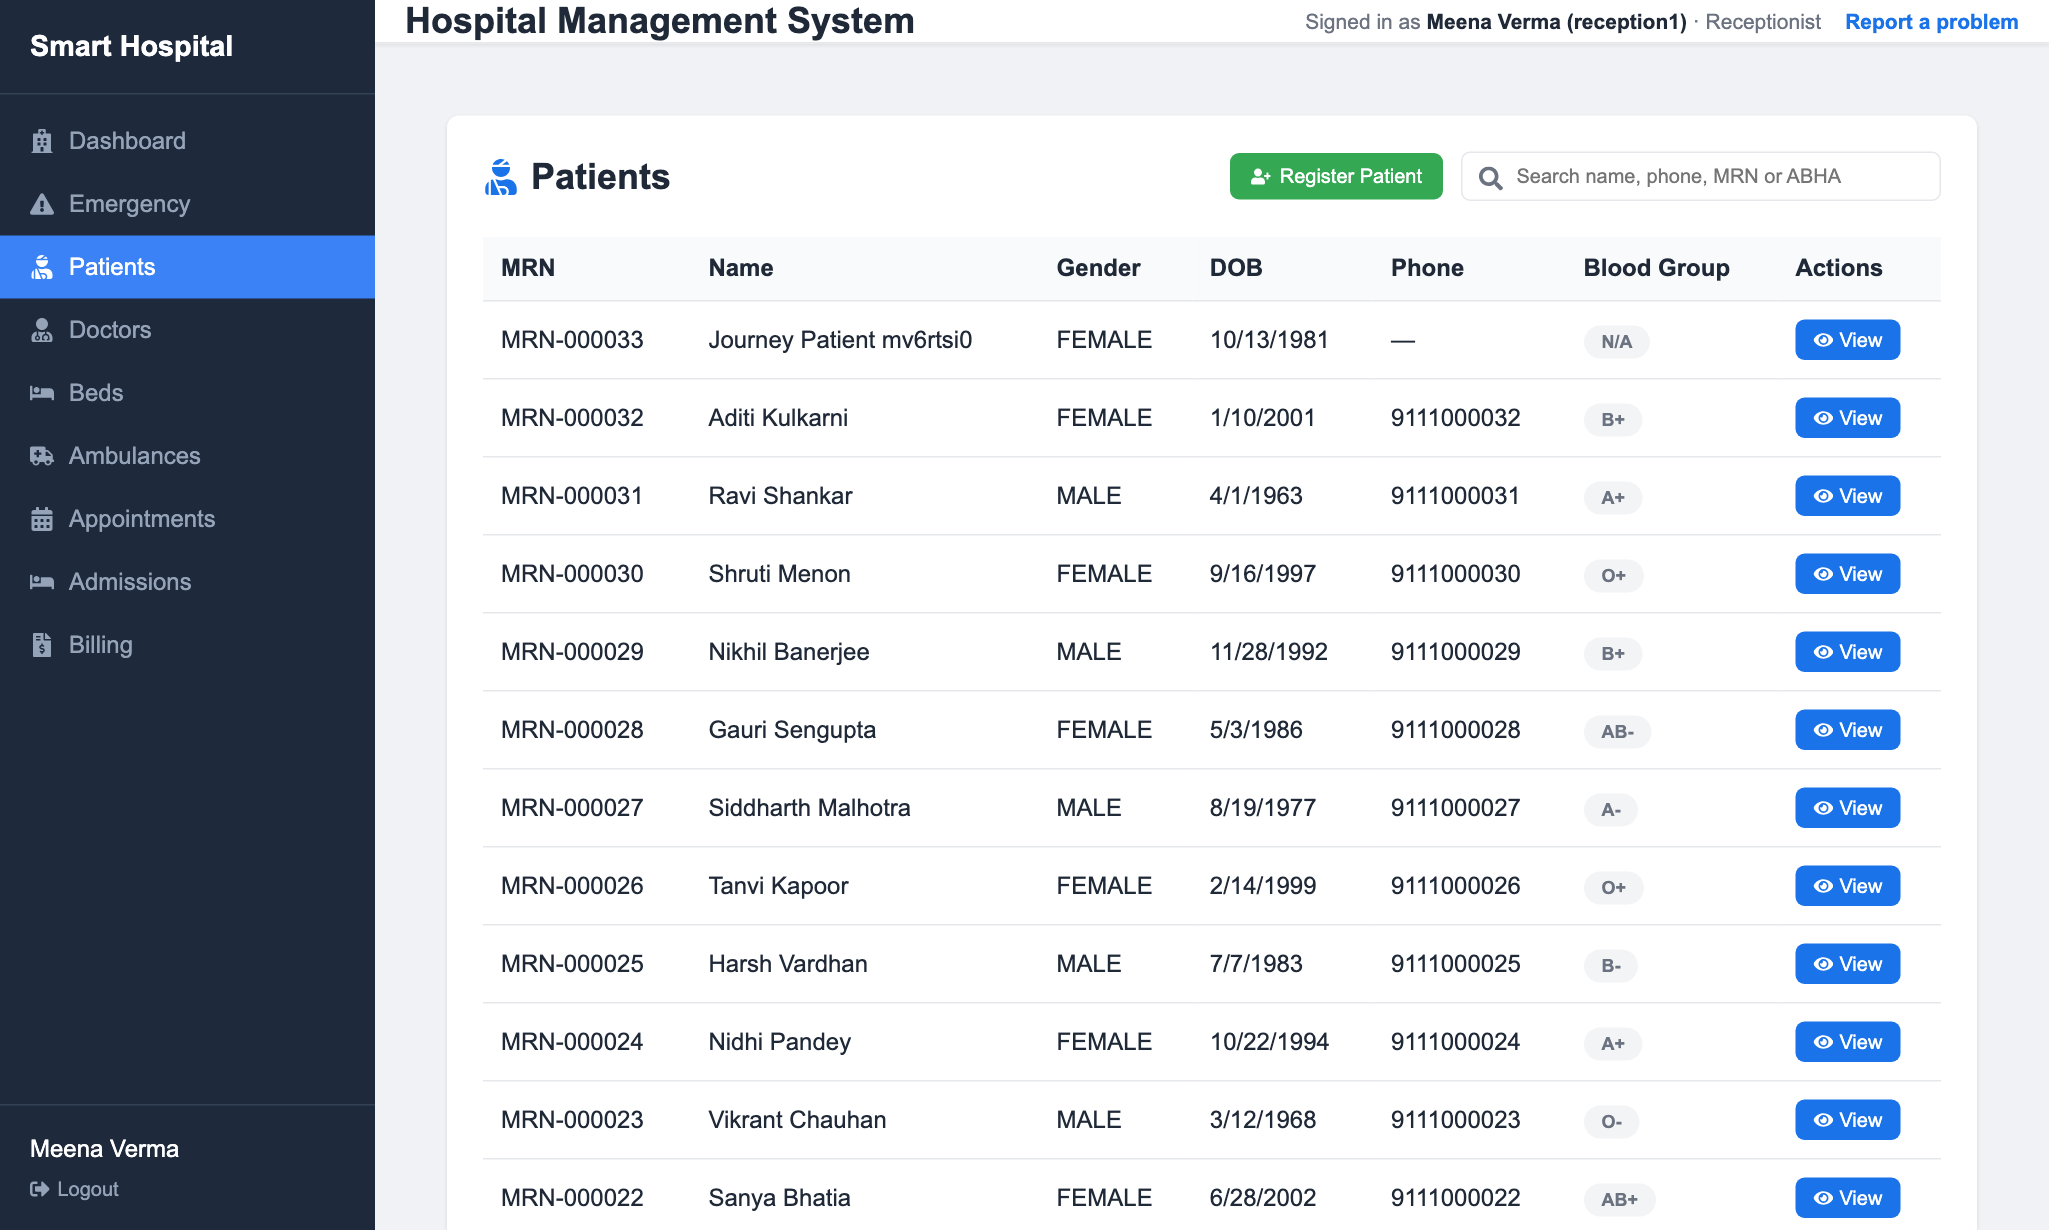
\includegraphics[width=0.485\textwidth]{reception-patients.png} & 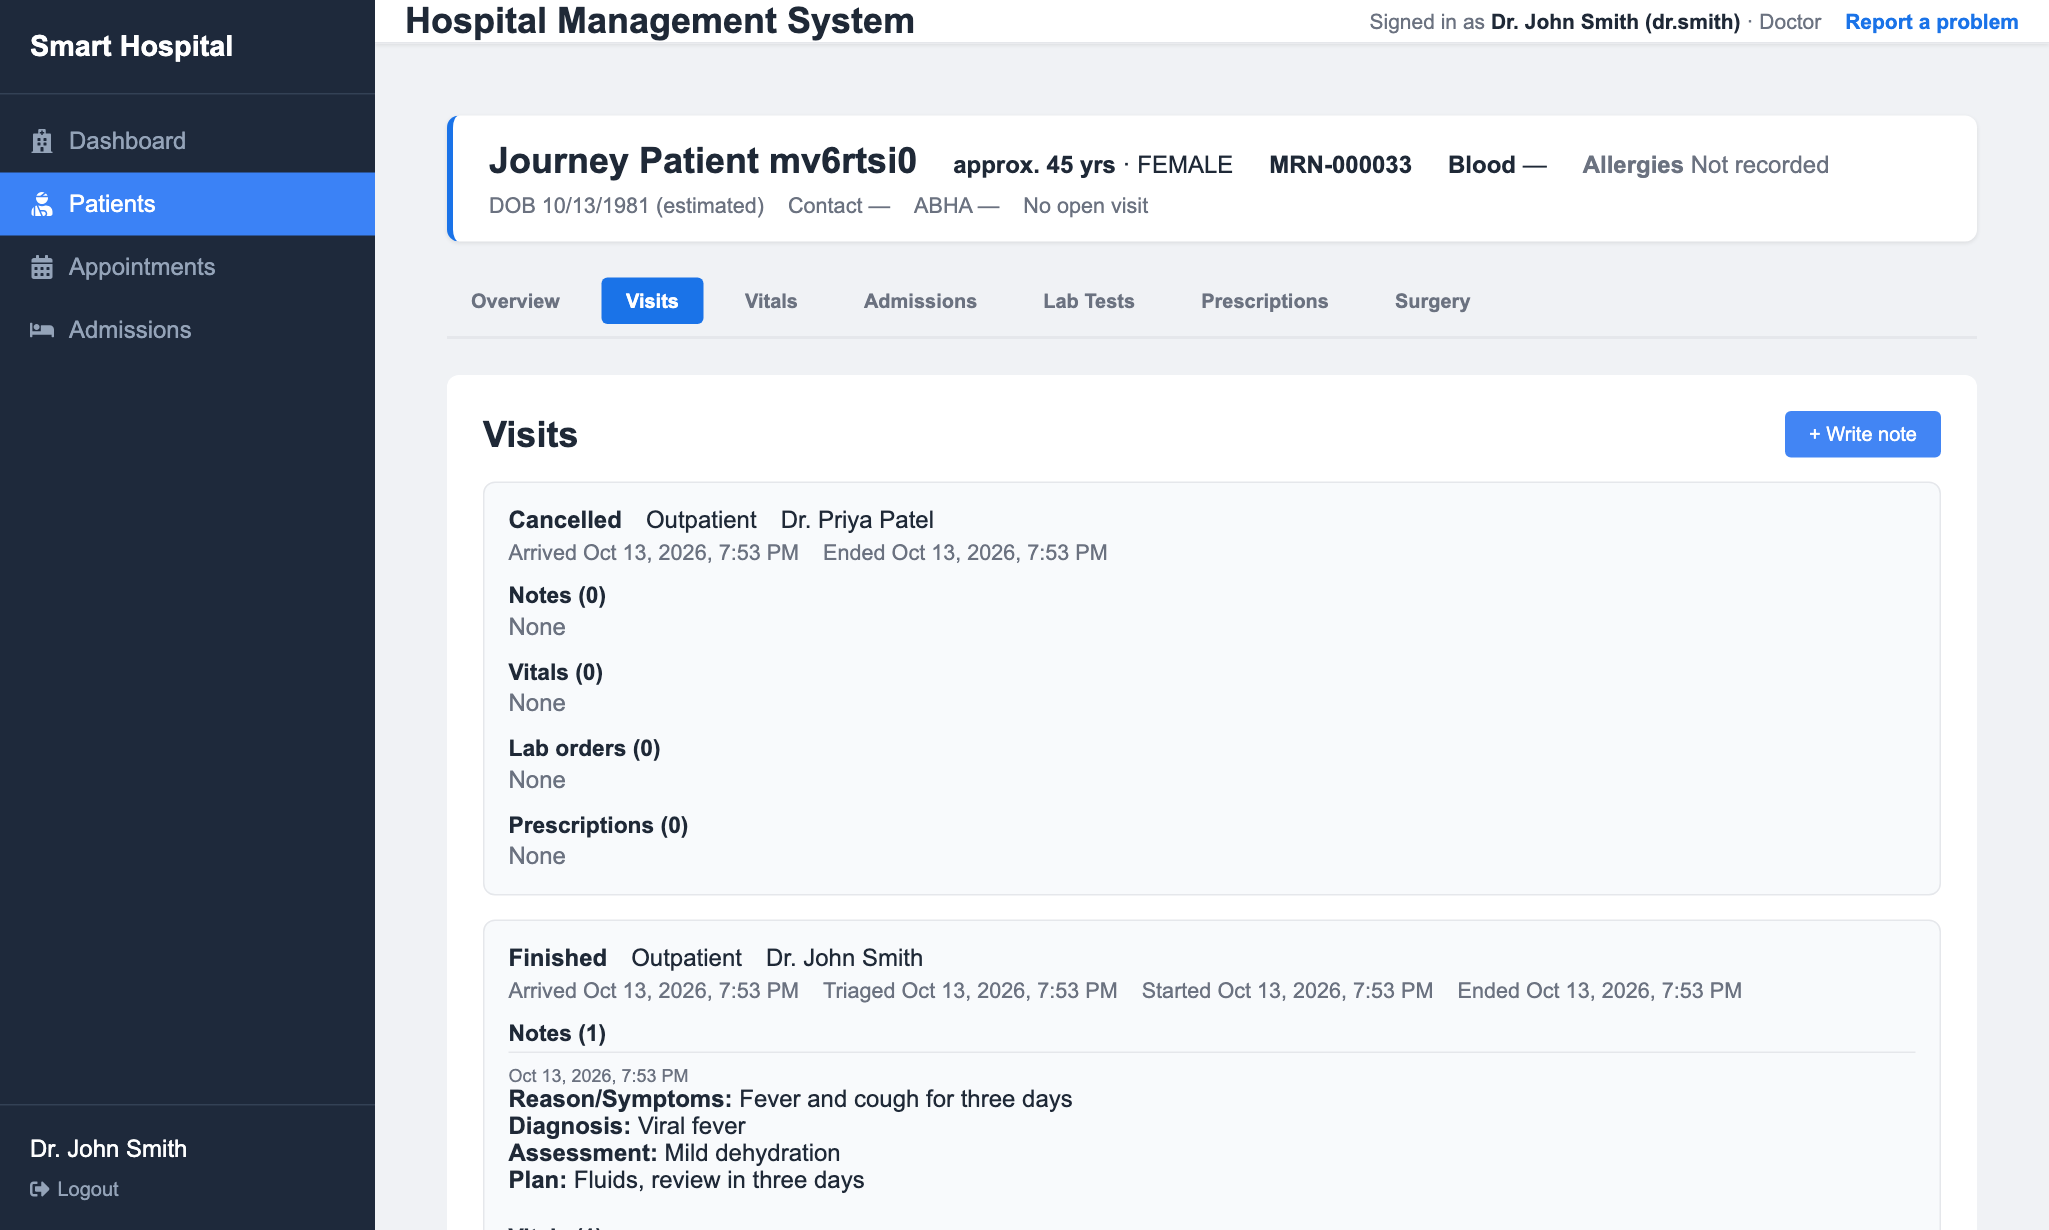
\includegraphics[width=0.485\textwidth]{doctor-patient.png} \\
\small (a) Receptionist: patient list and search & \small (b) Doctor: a patient's visits, notes and orders \\[3pt]
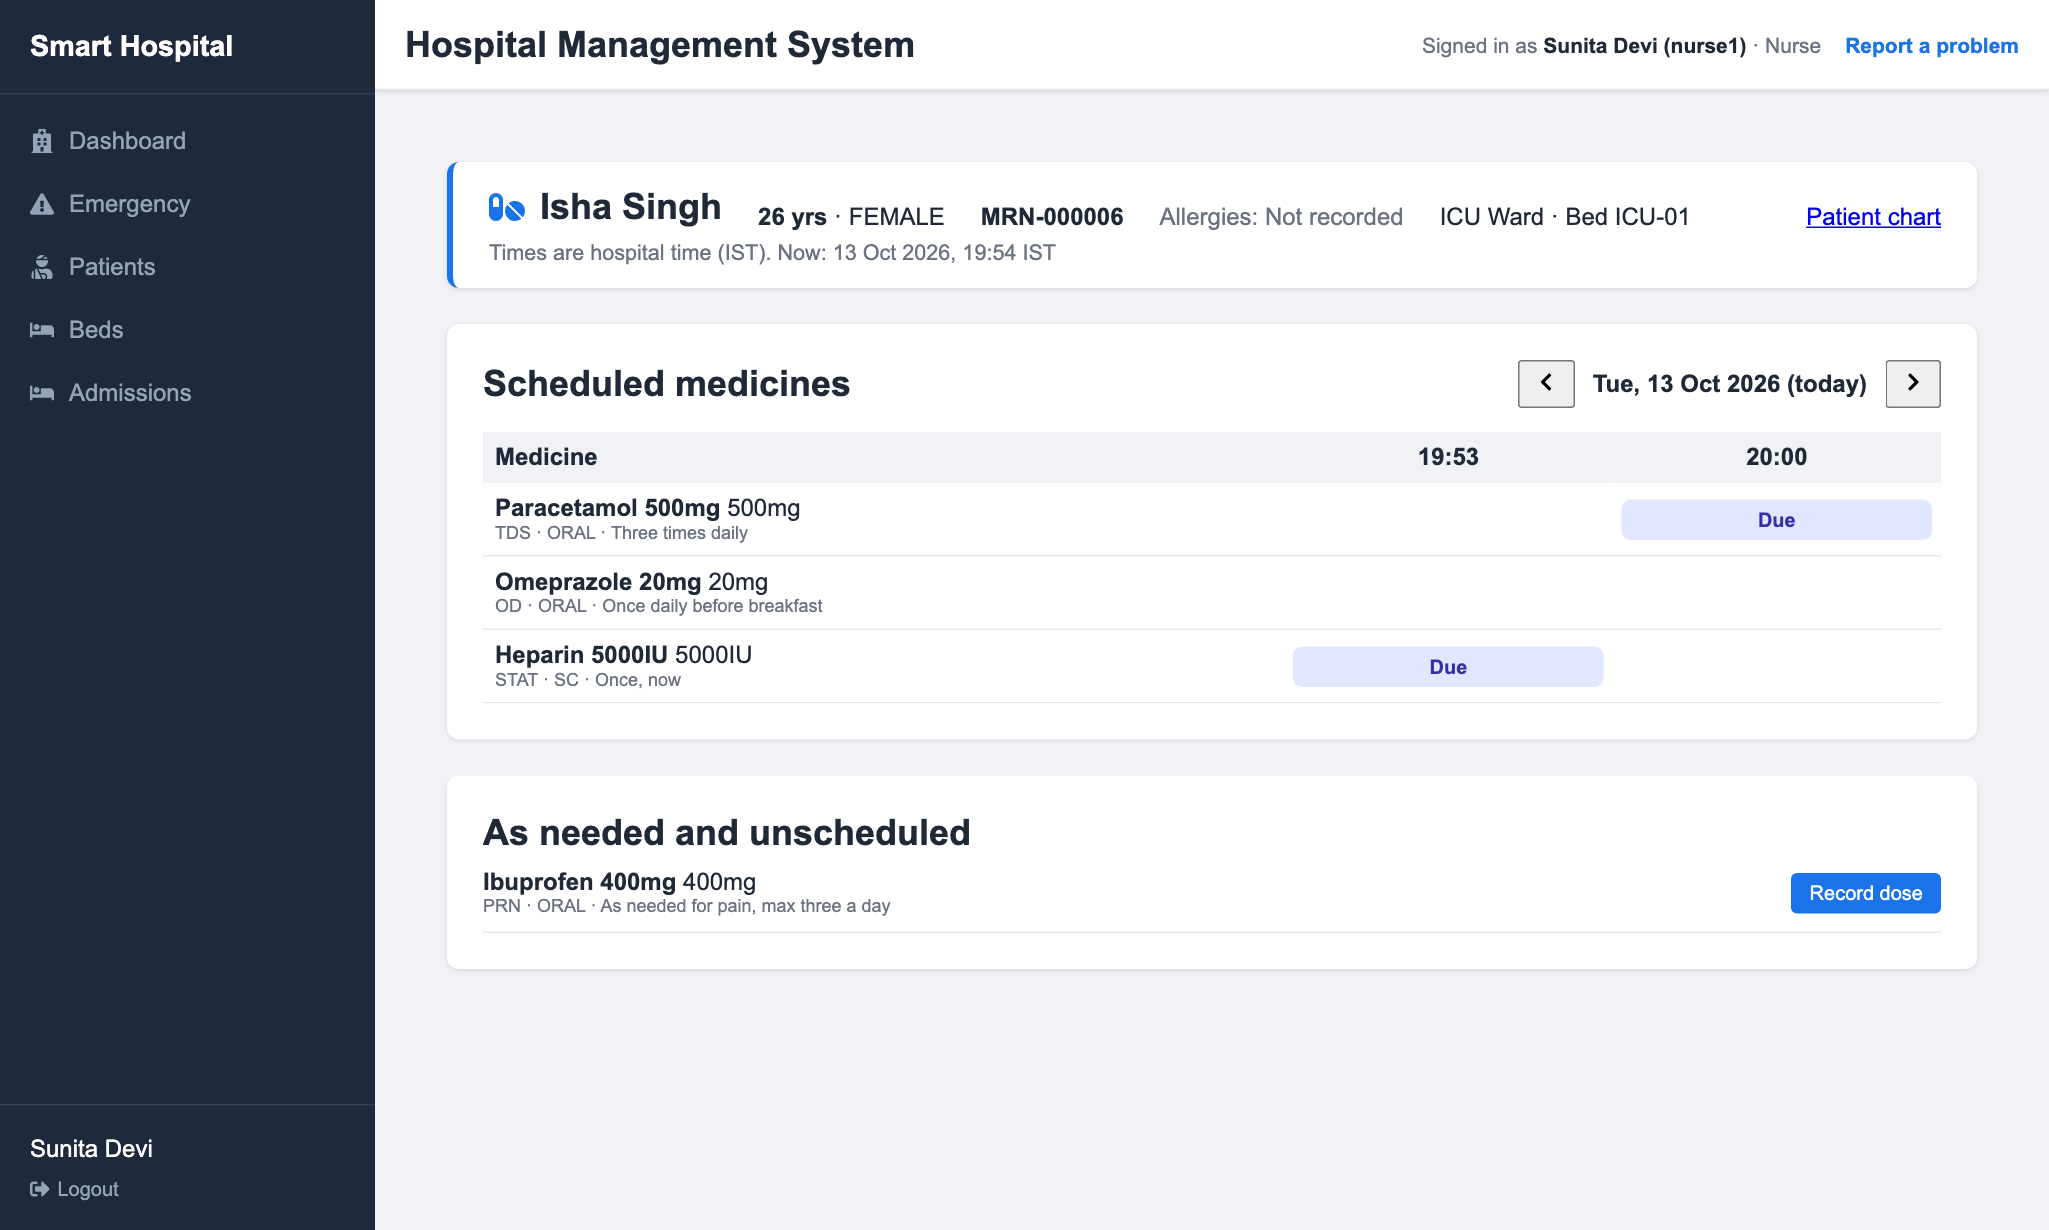
\includegraphics[width=0.485\textwidth]{nurse-mar.png} & 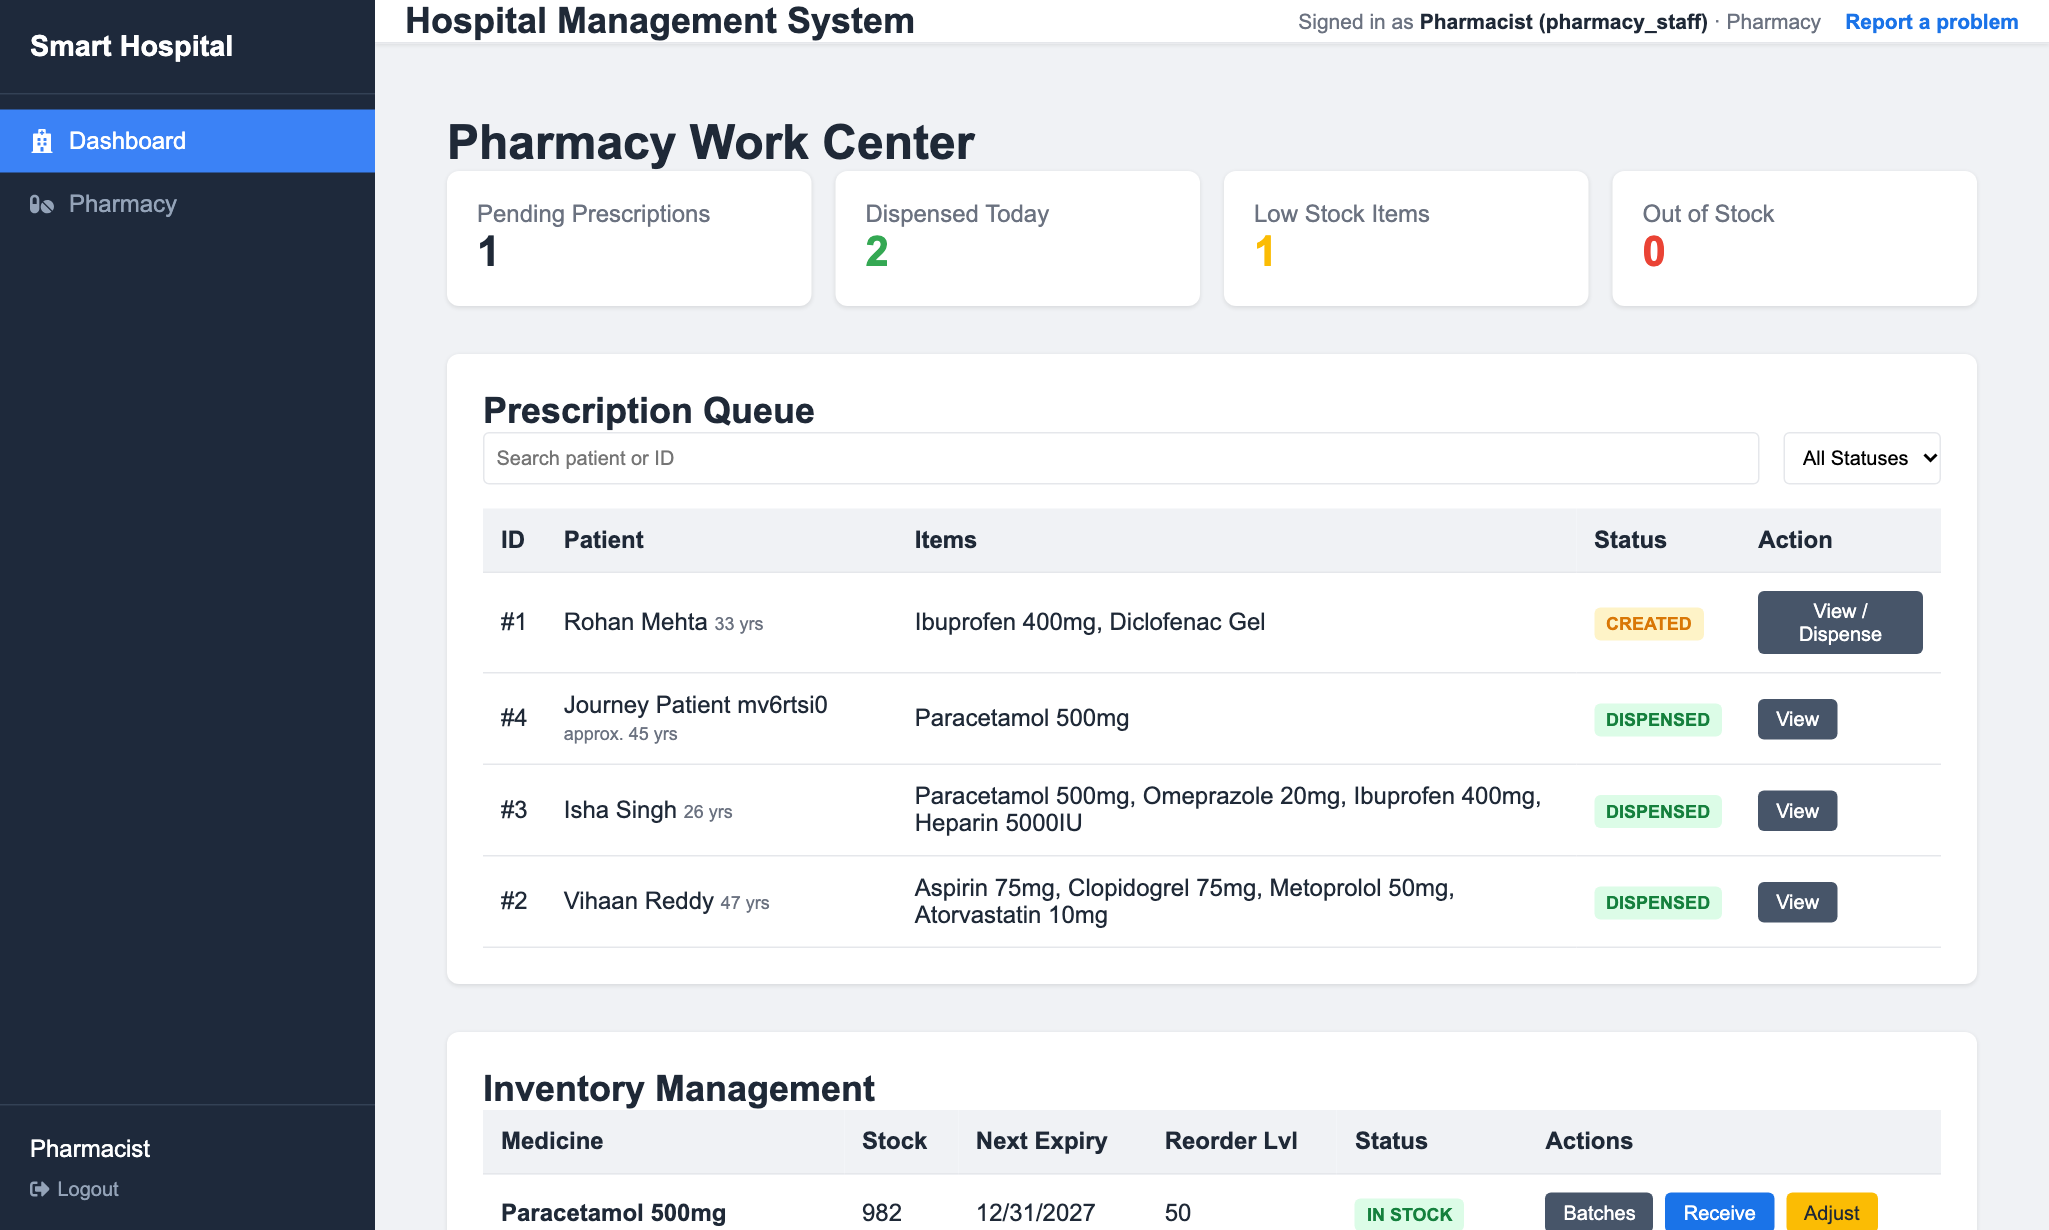
\includegraphics[width=0.485\textwidth]{pharmacy-dashboard.png} \\
\small (c) Nurse: medication administration record & \small (d) Pharmacy: dispense queue and stock \\
\end{tabular}
\caption{Major screens, one per role (test data)}\label{fig:screens}
\end{figure}

\section{Database Operations through the Application}
Each screen action becomes SQL in one transaction, and the result is visible in MySQL. The patient-journey browser
test drives these screens and then checks the rows in the database.

{\small
\begin{tabularx}{\textwidth}{@{}R{4.6cm}Y@{}}
\toprule
\textbf{Action on screen} & \textbf{Statements on hospital\_db} \\\midrule
Register a patient (reception) & \tbl{INSERT INTO patients}; \tbl{INSERT INTO audit\_logs} (CREATE\_PATIENT) \\
Book an appointment & \tbl{INSERT INTO appointments} (a duplicate slot fails the UNIQUE key: 409 ``Double booking detected'') \\
Mark arrived, start, finish a visit & \tbl{SELECT \dots{} FOR UPDATE} on the appointment and encounter; \tbl{INSERT}/\tbl{UPDATE encounters}; \tbl{UPDATE appointments SET status} \\
Record vital signs (nurse) & \tbl{INSERT INTO vital\_signs} (refused by the CHECKs if out of range) \\
Dispense (pharmacy) & Listing in Section~8.7: locks, \tbl{UPDATE} items and batches, \tbl{INSERT} movements \\
Admit, discharge (doctor) & \tbl{INSERT INTO admissions} / \tbl{UPDATE admissions SET status = 'DISCHARGED'}; triggers update the bed, the workload and \tbl{bed\_assignment\_log} \\
Edit a patient's details & \tbl{UPDATE patients}; the audit row names the changed fields, never their values \\
Cancel a prescription & \tbl{UPDATE prescriptions SET status = 'CANCELLED'}; pending doses \tbl{UPDATE medication\_administrations SET status = 'CANCELLED'} \\
Assign a nurse to a ward (admin) & \tbl{SELECT \dots{} FOR UPDATE} on the nurse's account, then on any assignment sharing a day (409 if one exists); \tbl{INSERT INTO nurse\_ward\_assignments} \\
End an assignment & \tbl{UPDATE nurse\_ward\_assignments SET end\_date = ?, ended\_at = ?}: the nurse loses the ward at once \\
Cancel an assignment not yet started & \tbl{DELETE FROM nurse\_ward\_assignments}, refused (409) once it has started \\
\bottomrule
\end{tabularx}}
Clinical records are not deleted through the application: they are kept, and corrections are recorded as new
states (for example a visit marked ENTERED\_IN\_ERROR), which the audit log requires. The one delete is cancelling a
nurse assignment before its first day, which never gave access to anything; the audit log keeps its dates.

\chapter{Testing and Results}

\section{Test Cases}
Each case was run against the API and database of the test environment; the actual result is the response or
MySQL error that came back.

{\scriptsize\setlength{\tabcolsep}{3pt}
\begin{longtable}{@{}R{0.55cm}R{2.2cm}R{3.6cm}R{2.3cm}R{6.9cm}R{0.6cm}@{}}
\caption{Test cases with their actual results}\label{tab:tests}\\
\toprule
\textbf{Test ID} & \textbf{Operation} & \textbf{Input} & \textbf{Expected Result} & \textbf{Actual Result} & \textbf{Status} \\\midrule\endfirsthead
\toprule\textbf{ID} & \textbf{Operation} & \textbf{Input} & \textbf{Expected} & \textbf{Actual} & \textbf{Status} \\\midrule\endhead
\rows{generated/test-cases.tex}
\bottomrule
\end{longtable}}

\section{Query Testing}
Each query of Section~8.6 was run on the test database and its output checked against the data. For example, the bed
totals agree (35 beds both by type in Query~13 and by ward in Table~\ref{tab:sample}), Query~6's LEFT JOIN
returns doctors with no active admission as 0 rather than dropping them, and Query~11's \tbl{> ALL} returns exactly
the medicines dearer than the most expensive antibiotic (25.00). The automated suite also tests the application's
own queries: for instance, that a doctor's patient list contains only patients in their care, and that every
medicine's total equals the sum of its batches after each stock test.

\section{Constraint Testing}
Cases T2 to T4, T6, T11 and T12 show the database refusing invalid data on its own (duplicate key, missing parent,
negative stock, duplicate ABHA, a dispense time without the flag, editing the audit log). T10 shows a composite
foreign key and the matching API check refusing a bill whose patient differs from its admission's patient.
The server suite contains a test for every constraint added in this work, run on the database itself.

\section{Results and Discussion}
\begin{itemize}
\item \textbf{Server suite:} 303 tests in 46 files (\texttt{node:test}) against a server on \tbl{hospital\_db\_test}, which is rebuilt from the migrations for every run: all pass.
\item \textbf{Time of day:} the same checks run against servers whose clocks read 00:30 IST (when the UTC date is still the day before) and 06:00 IST: nurse assignment status, a nurse's access, today's appointments and counts, ages and expiry agree at both times.
\item \textbf{Browser suite:} 121 tests in 29 files (Puppeteer) driving every role's screens: all pass, with the test machine's time zone set to India, UTC and Los Angeles in turn.
\item \textbf{Stress test:} 300 rounds of competing prescribing and dispensing, and 300 rounds of mixed writers: 0 deadlocks, stock consistent.
\item \textbf{Patient journey:} 13 steps from registration to discharge across five roles (every role but laboratory): all pass locally.
\end{itemize}
One defect was found while preparing this report: \tbl{POST /api/patients} answers HTTP 500 instead of saving
when the request omits the optional fields (blood group, phone, address, emergency contact), because the missing
values reach MySQL as \texttt{undefined}. The registration form always sends them, so users are not affected; it is
listed as a limitation and was not changed for this report.

\chapter{Conclusion and Future Scope}

\section{Conclusion}
The project models a hospital's operations as 30 entities and 69 relationships, maps them to 33 MySQL tables, and
normalizes them: 24 tables are in BCNF, and the 9 that keep a copied value have that copy enforced by composite
foreign keys or a CHECK constraint. The rules of the hospital live in the database (87 foreign keys, 23 unique keys,
30 CHECKs, 7 triggers, row locking in a fixed order), and a role-based React and Express application uses it through
a restricted account. Automated tests confirm the behaviour, including under concurrency.

\section{Limitations}
\begin{itemize}
\item A lab order stores one result value: multi-analyte panels (a lipid profile's four values) are recorded as text in one result.
\item The ABHA number is stored and validated for format and uniqueness only; there is no live integration with the national ABDM network.
\item Allergies are free text in one column, not a separate table, so they cannot be checked against a prescription automatically.
\item Bed transfers within one admission are not modelled; an admission has one bed.
\item \tbl{POST /api/patients} returns HTTP 500 when optional fields are omitted from the request (Section~10.4).
\item Seven of the ten views and the five stored procedures come from the original schema and are not used by the API.
\item One hospital only; no payment gateway or insurance claims.
\end{itemize}

\section{Future Scope}
\begin{itemize}
\item Panel results (one row per analyte) and a structured allergy list checked at prescribing time.
\item ABDM integration: verify ABHA numbers and exchange health records with consent.
\item Bed transfers, with the bed history as the source of truth for where a patient is.
\item Payments and insurance claims; dashboards over the audit log and the daily statistics.
\end{itemize}

\chapter*{References}
\addcontentsline{toc}{chapter}{References}
\begin{enumerate}[label={[\arabic*]}, leftmargin=2em]
\item R.~Elmasri and S.~B.~Navathe, \emph{Fundamentals of Database Systems}, 7th~ed. Pearson, 2016.
\item A.~Silberschatz, H.~F.~Korth and S.~Sudarshan, \emph{Database System Concepts}, 7th~ed. McGraw-Hill, 2019.
\item P.~P.-S.~Chen, ``The entity-relationship model: toward a unified view of data,'' \emph{ACM Transactions on Database Systems}, vol.~1, no.~1, pp.~9--36, 1976.
\item E.~F.~Codd, ``A relational model of data for large shared data banks,'' \emph{Communications of the ACM}, vol.~13, no.~6, pp.~377--387, 1970.
\item Oracle, \emph{MySQL 9.7 Reference Manual}, chapters on InnoDB locking, foreign keys, CHECK constraints, generated columns and triggers. [Online]. Available: \url{https://dev.mysql.com/doc/}
\item OpenJS Foundation, \emph{Node.js Documentation} (including the \texttt{node:test} runner). [Online]. Available: \url{https://nodejs.org/docs/}
\item \emph{Express 4 API Reference}. [Online]. Available: \url{https://expressjs.com/}
\item Meta, \emph{React Documentation}. [Online]. Available: \url{https://react.dev/}
\item \emph{mysql2 for Node.js}. [Online]. Available: \url{https://sidorares.github.io/node-mysql2/docs}
\item Google, \emph{Puppeteer Documentation}. [Online]. Available: \url{https://pptr.dev/}
\item National Health Authority, \emph{Ayushman Bharat Digital Mission: ABHA number}. [Online]. Available: \url{https://abdm.gov.in/}
\end{enumerate}

\clearpage
\appendix
\chapter{Complete MySQL Script}
The complete script is supplied as a separate file with this report: \textbf{\texttt{docs/report/hospital\_db\_full.sql}}
(about 130 KB). It was exported with \texttt{mysqldump} from a database built from \texttt{database/seed.sql} and
migrations 000--023, the same schema as \texttt{hospital\_db}, and contains, in order:
\begin{itemize}
\item \texttt{CREATE DATABASE hospital\_db} (utf8mb4) and \texttt{USE hospital\_db};
\item the 33 \texttt{CREATE TABLE} statements with every primary key, foreign key (including the 15 composite consistency keys), UNIQUE key, CHECK constraint, index and the generated column;
\item the sample data as \texttt{INSERT} statements (all people in it are made up; account passwords are bcrypt hashes of the documented demo password);
\item the 10 views, 7 triggers and 5 stored procedures.
\end{itemize}
Load it with \texttt{mysql -u root -p < hospital\_db\_full.sql}. Loaded into an empty server, it produced a database
whose structure matched \texttt{hospital\_db} exactly (schema-diff: no differences). The queries of Section~8.6 are in
\texttt{docs/report/generated/q1.sql} to \texttt{q15.sql}, and the migrations that build the schema step by step are in
\texttt{database/migrations/}.

\chapter{Source Code}
The source code is in the GitHub repository
\textbf{\url{https://github.com/rohithsaivemuri-sudo/hospital-dashboard}} (branch \texttt{main}):
\begin{itemize}
\item \texttt{server/}: the Express API (routes, controllers, services, middleware), migration and test scripts, and the automated tests (\texttt{server/tests});
\item \texttt{client/}: the React application (\texttt{client/src/pages} has one folder per module);
\item \texttt{database/}: the migrations and the seed data;
\item \texttt{tests/ui/}: the browser tests; \texttt{deploy/azure/}: deployment scripts;
\item \texttt{docs/}: this report and its source (\texttt{docs/report}), the BCNF analysis, the database report and the editable ER diagrams (\texttt{er-diagrams.drawio}).
\end{itemize}
A demonstration copy runs at \url{https://hms-demo-in.indonesiacentral.cloudapp.azure.com} (sign-in required).

\chapter{Additional Screenshots}
\begin{figure}[H]\centering
\begin{tabular}{@{}cc@{}}
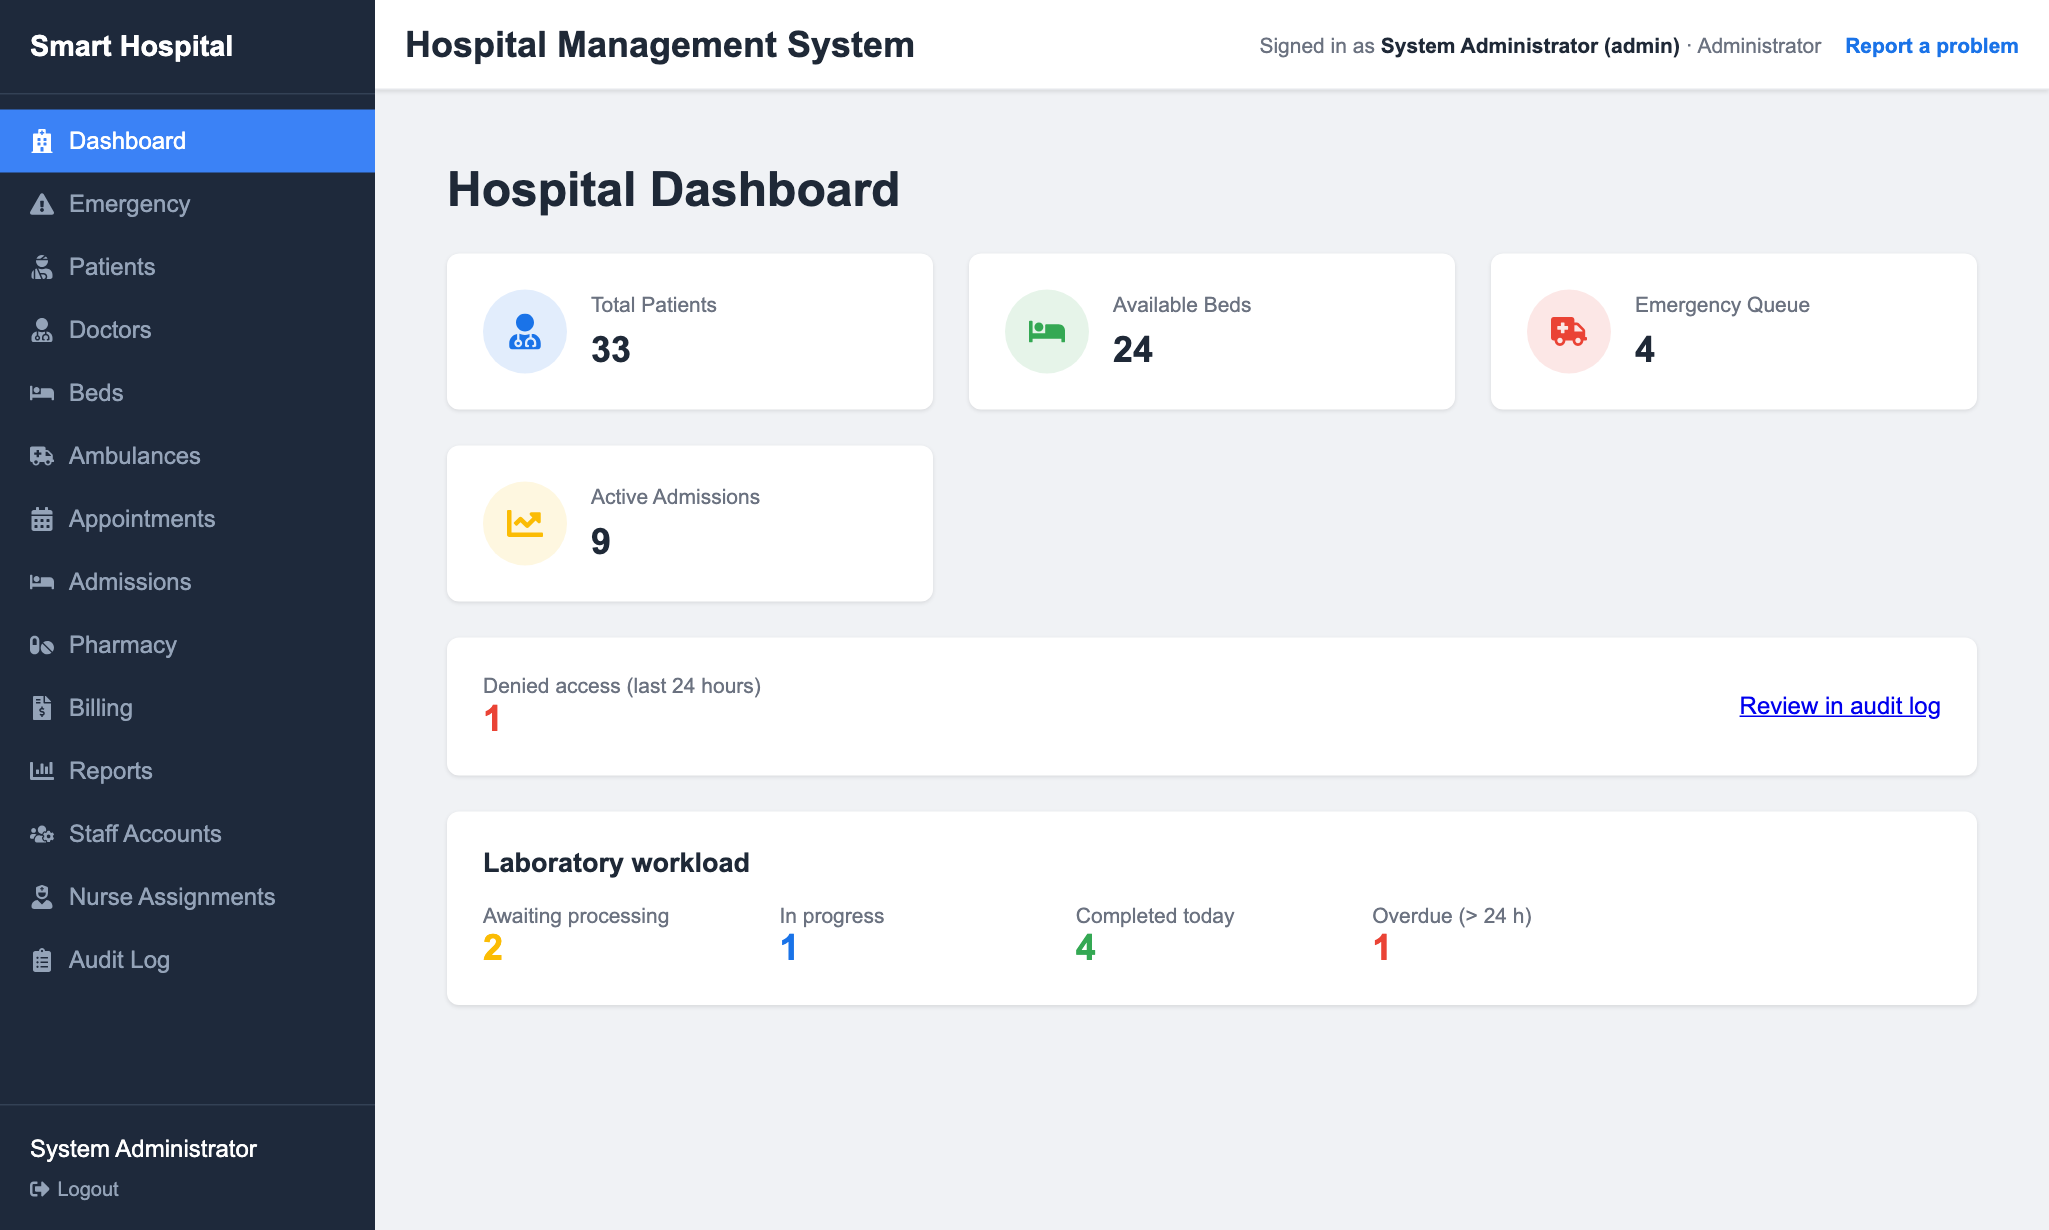
\includegraphics[width=0.485\textwidth]{admin-dashboard.png} & 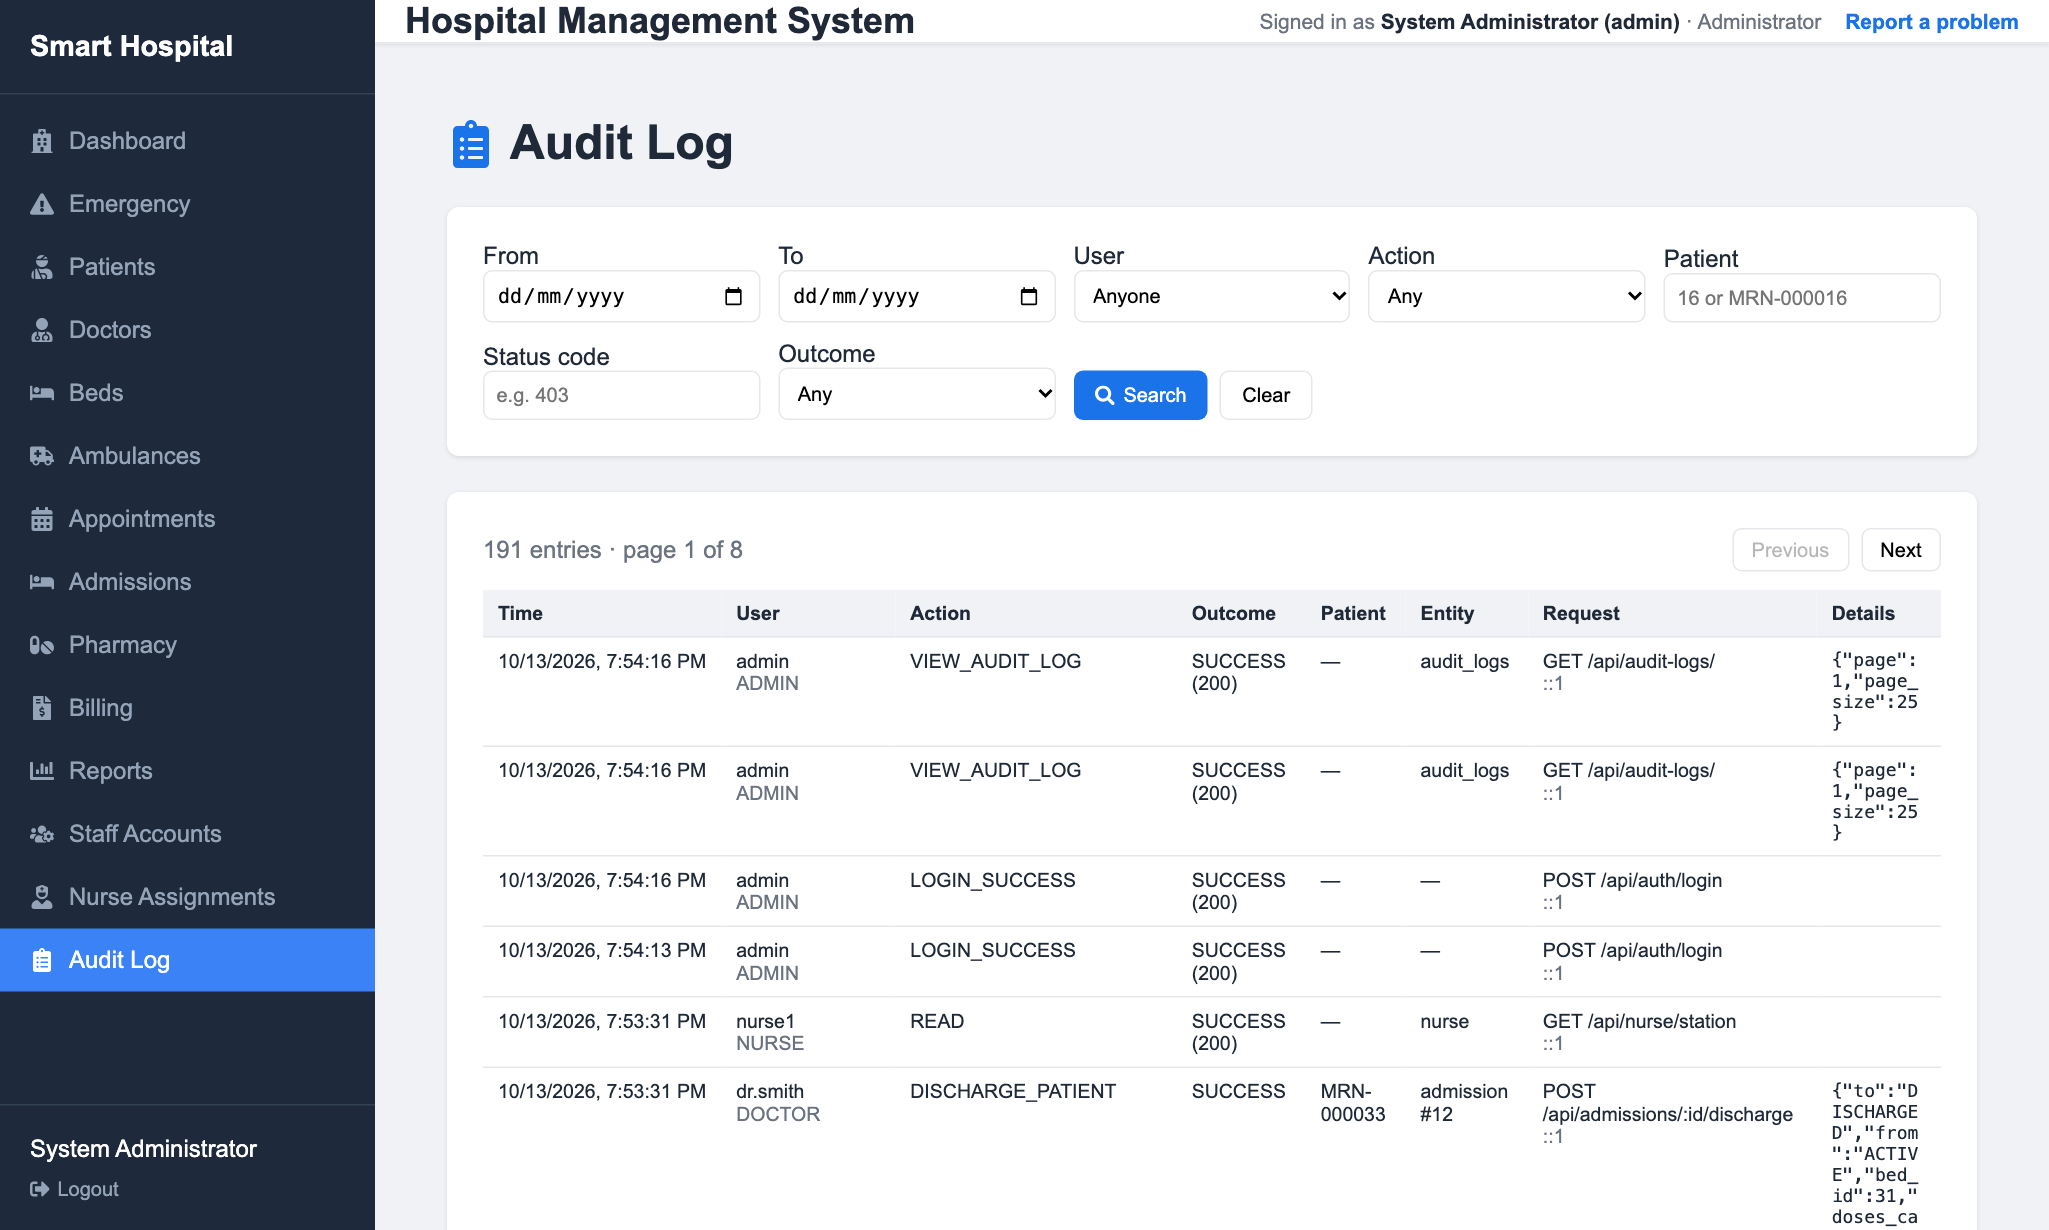
\includegraphics[width=0.485\textwidth]{admin-audit.png} \\
\small (a) Administrator: hospital dashboard & \small (b) Administrator: audit log \\[3pt]
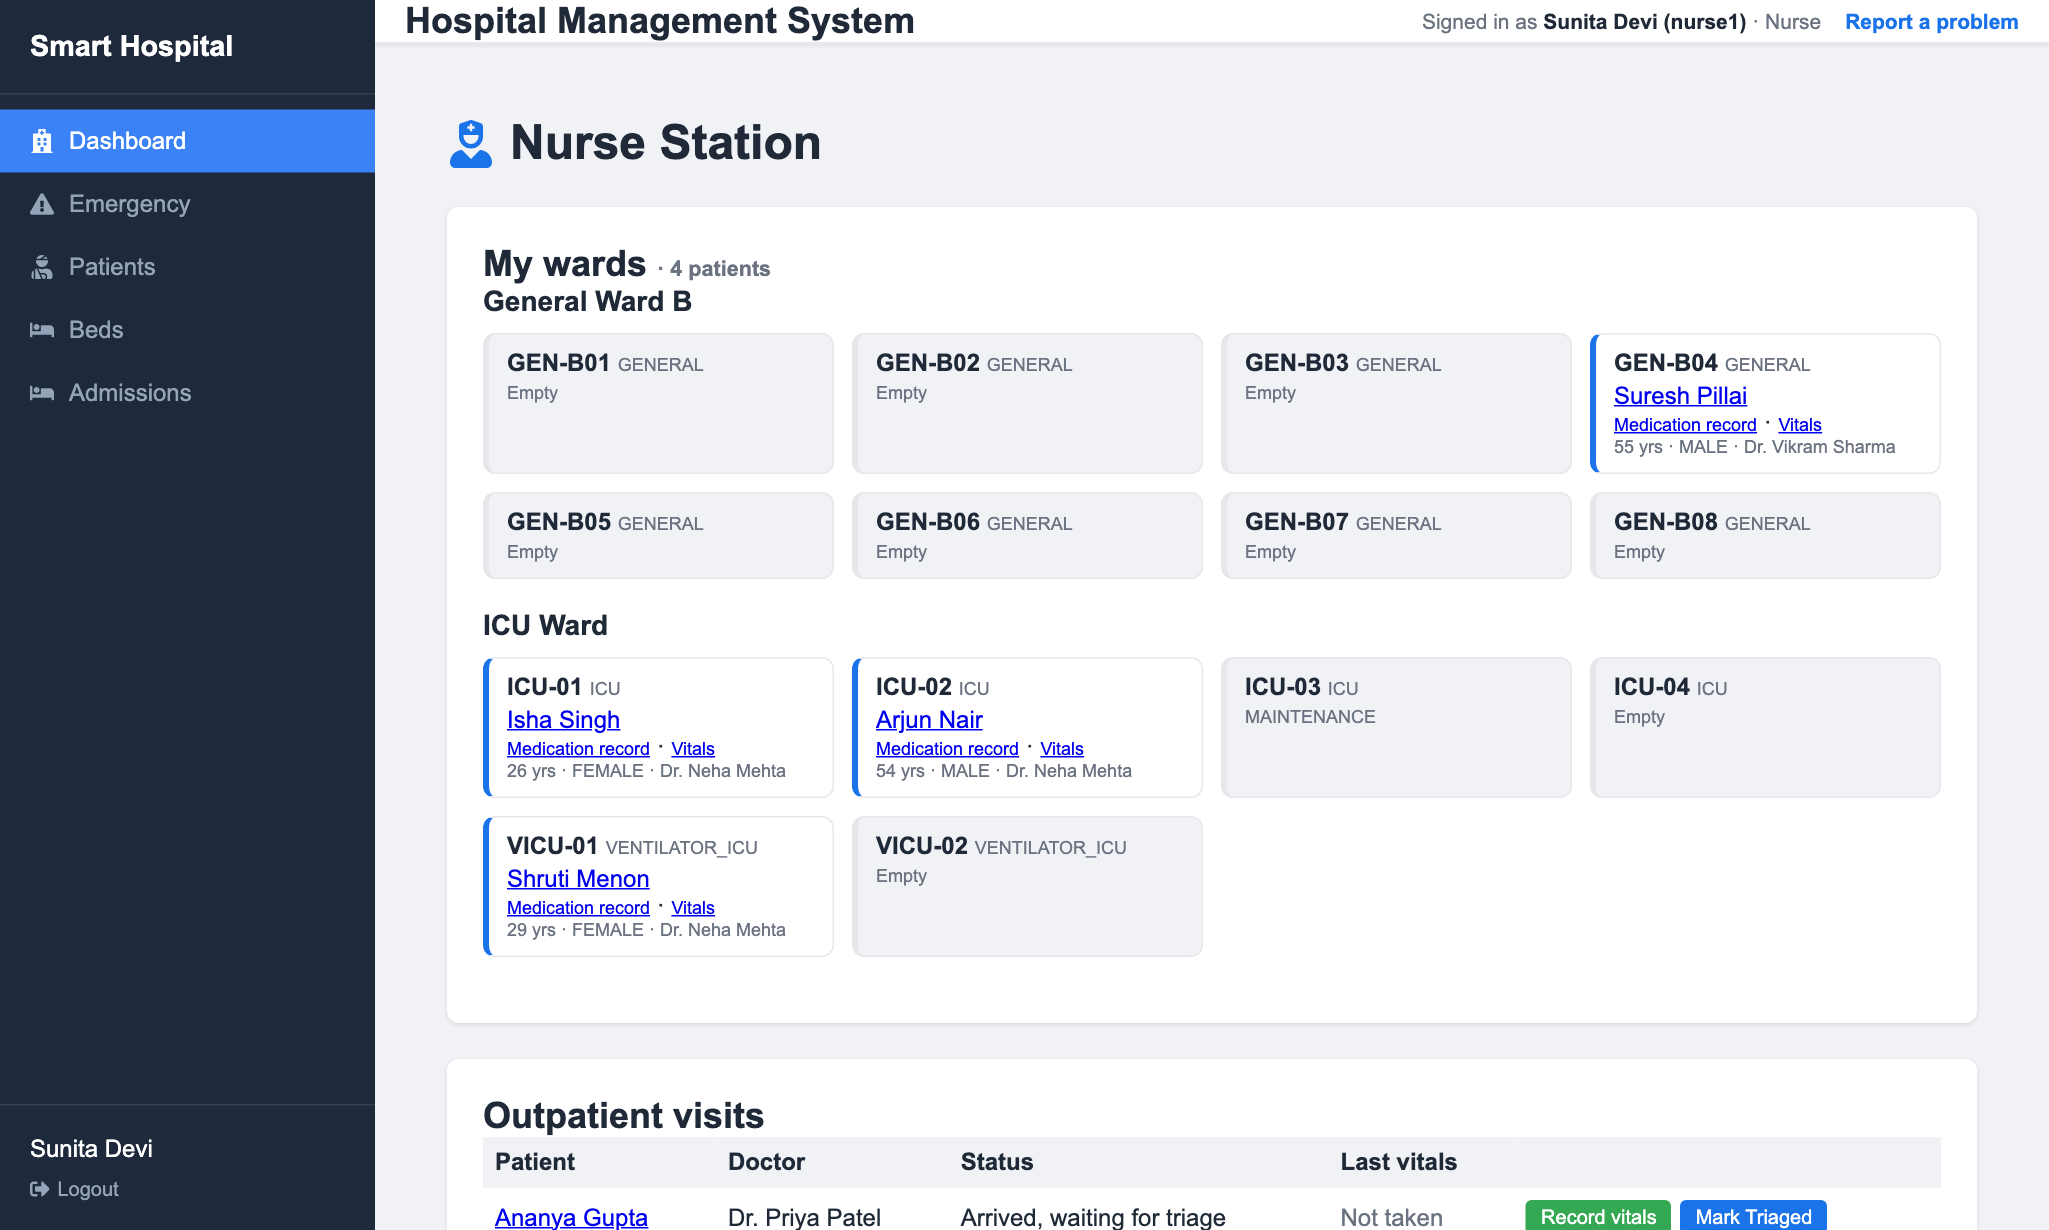
\includegraphics[width=0.485\textwidth]{nurse-station.png} & 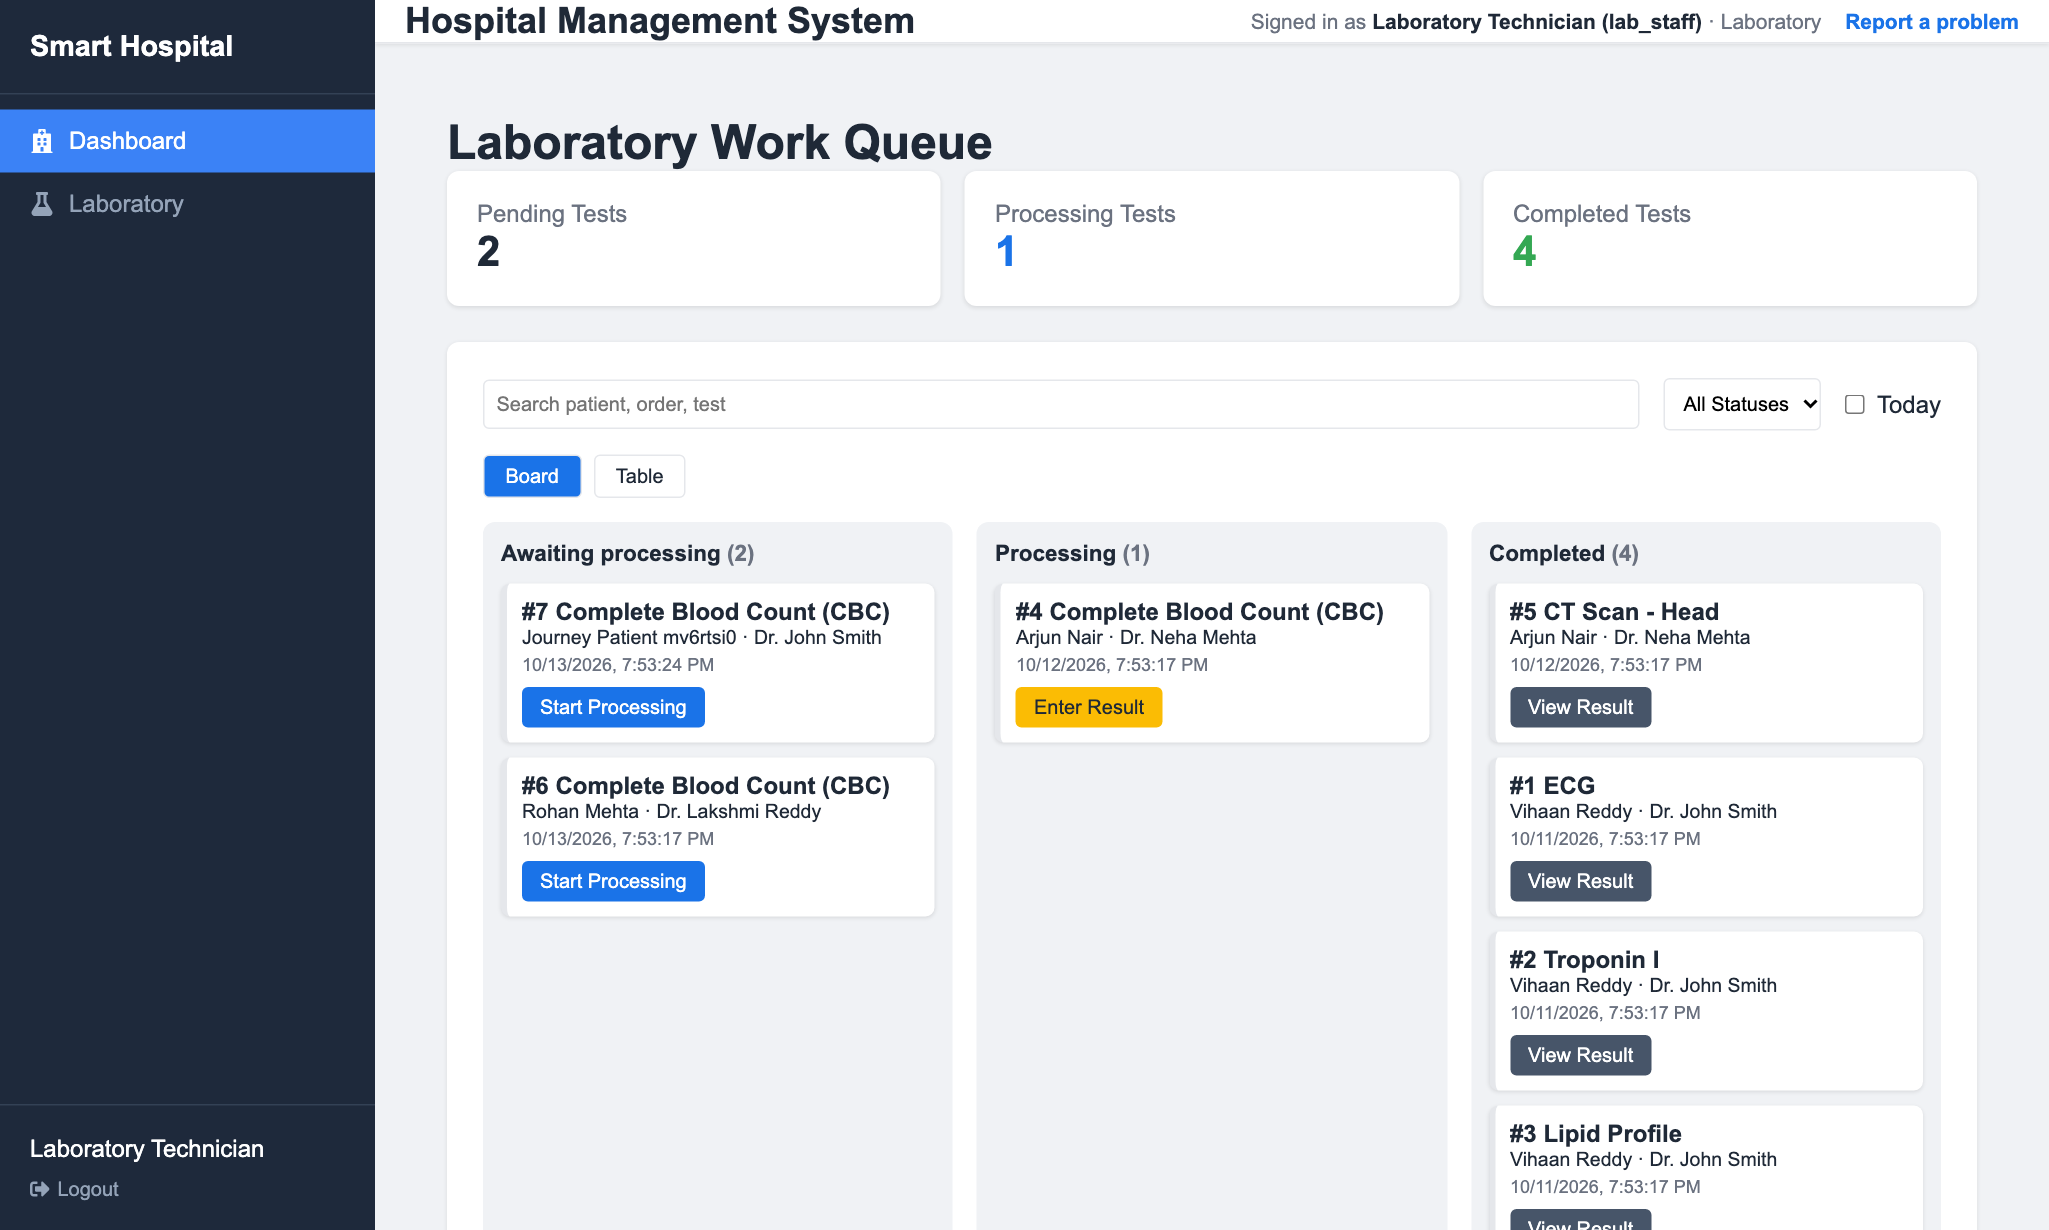
\includegraphics[width=0.485\textwidth]{lab-dashboard.png} \\
\small (c) Nurse: ward station with assigned beds & \small (d) Laboratory: order board \\[3pt]
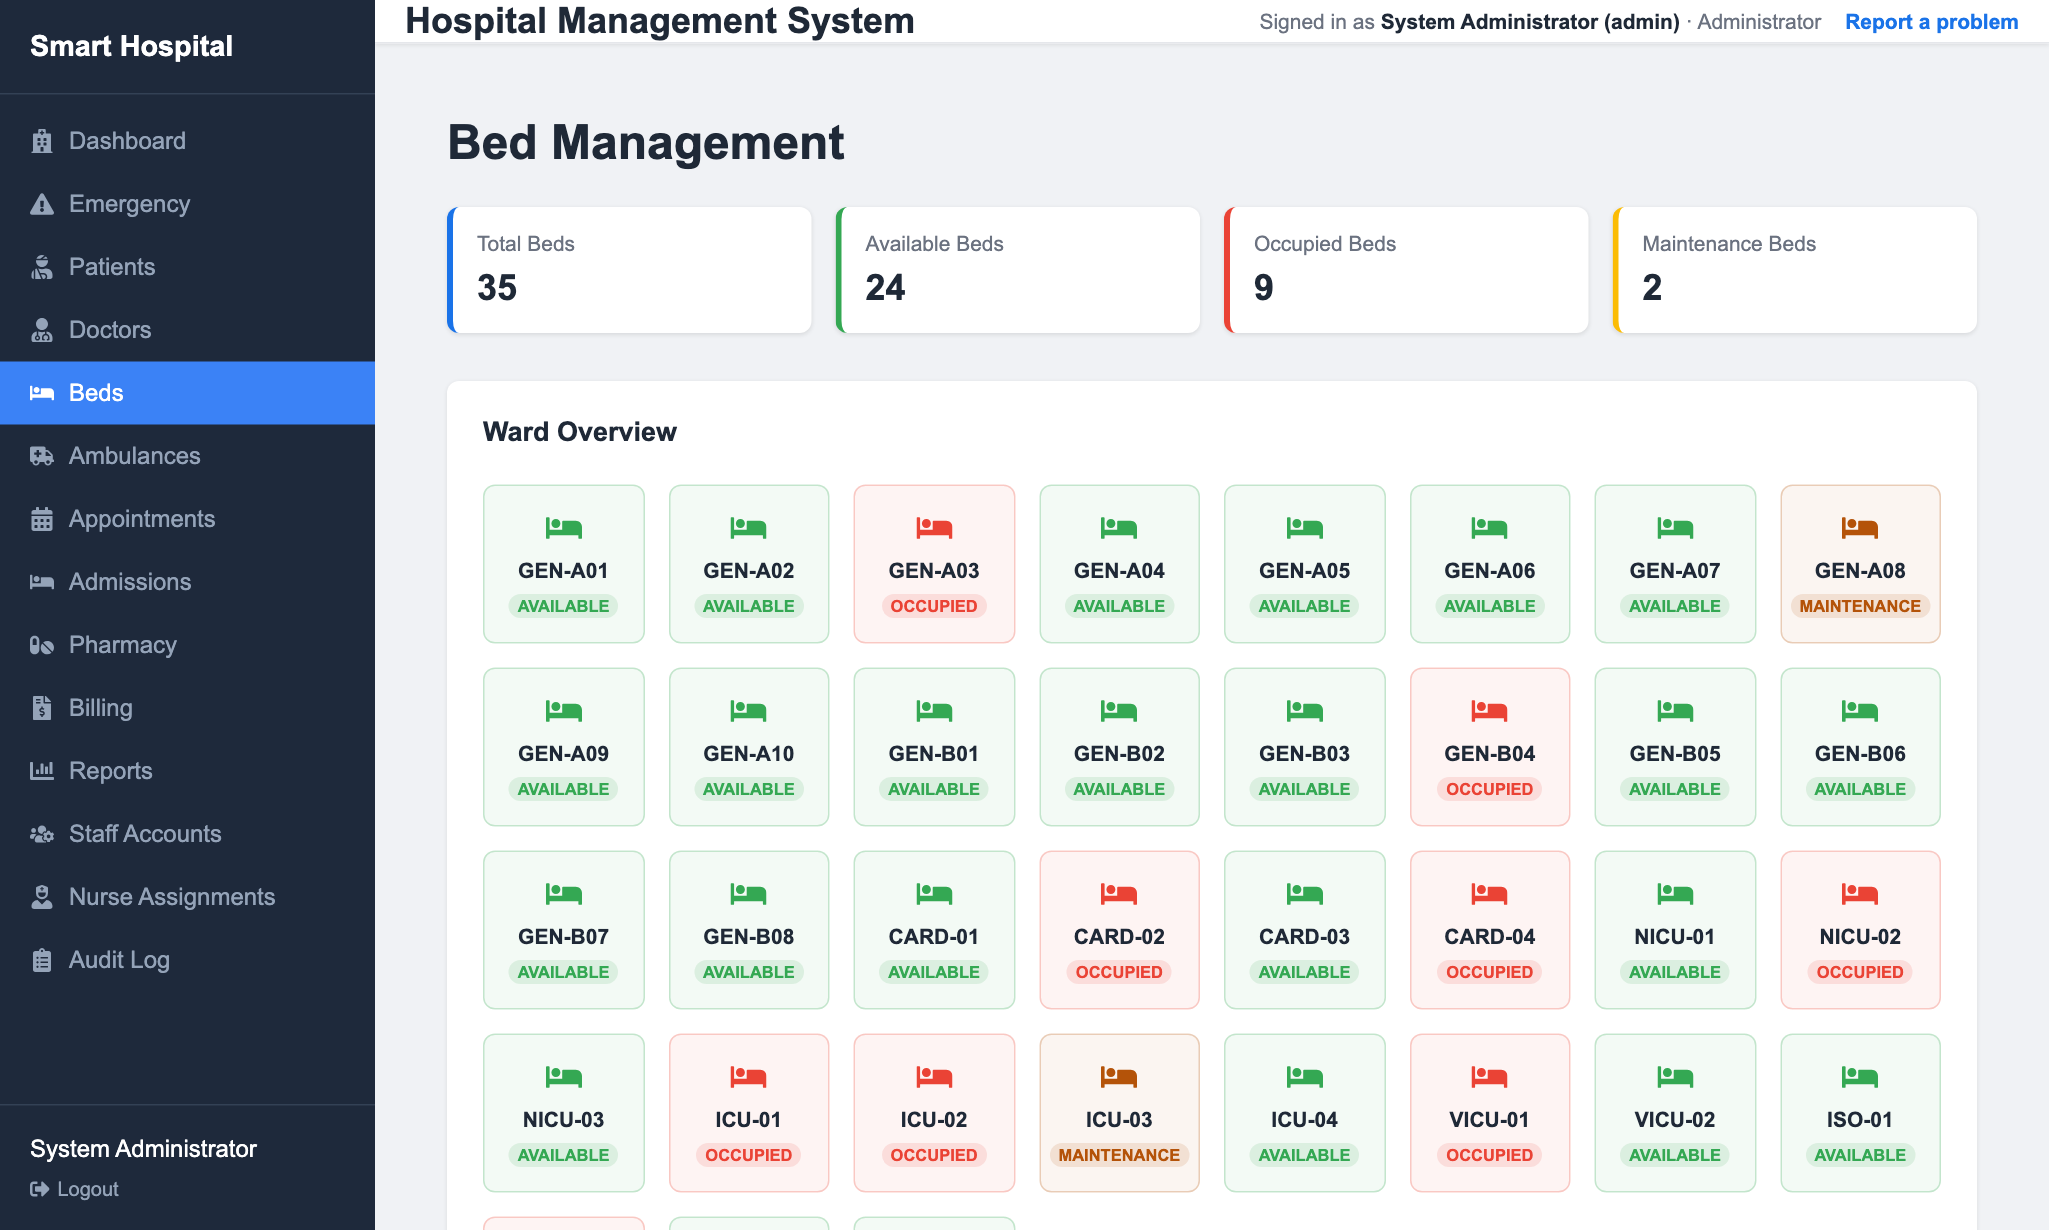
\includegraphics[width=0.485\textwidth]{admin-beds.png} & 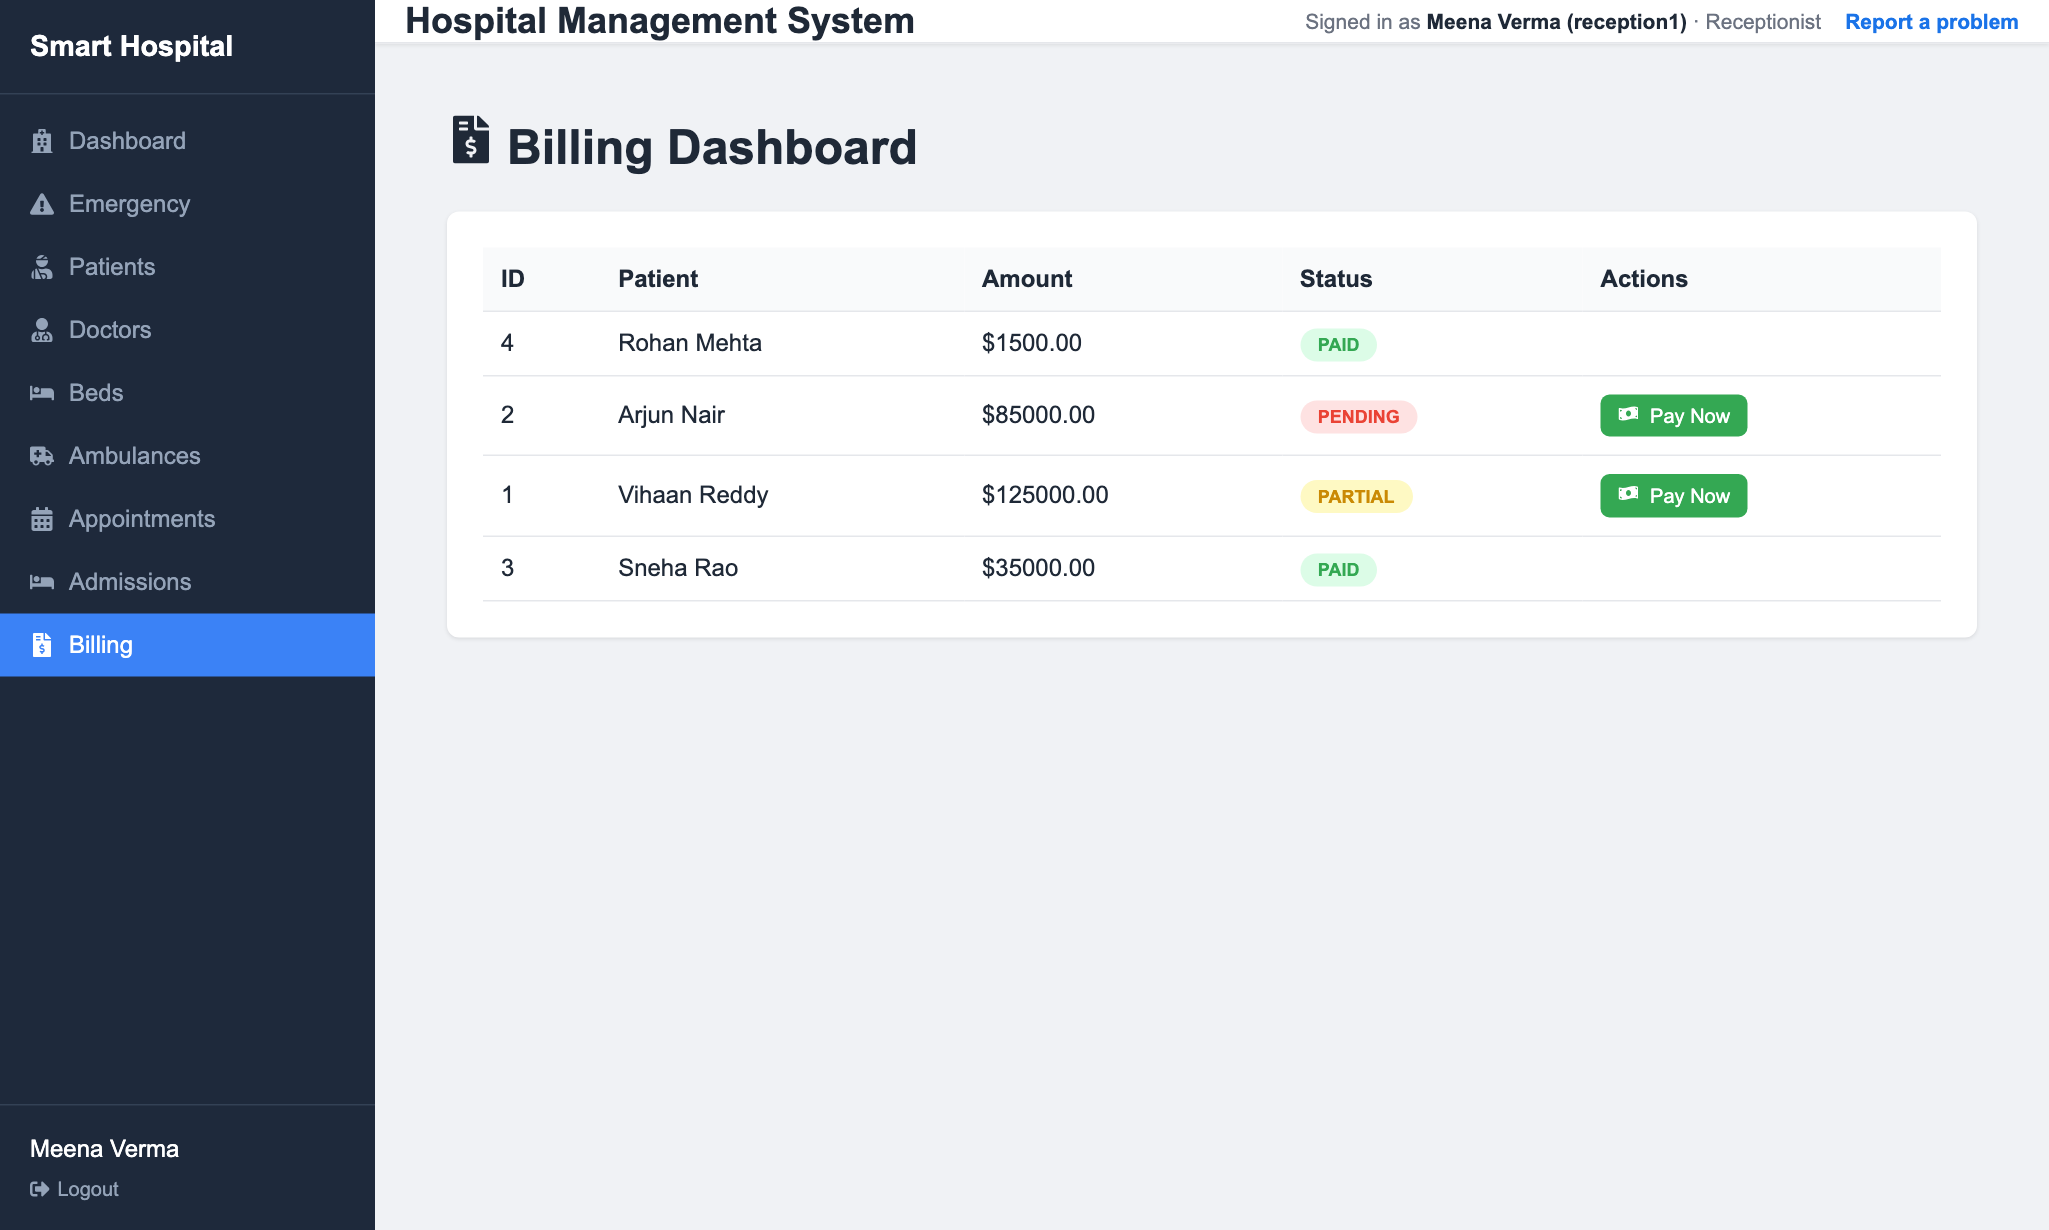
\includegraphics[width=0.485\textwidth]{reception-billing.png} \\
\small (e) Bed board & \small (f) Receptionist: billing \\
\end{tabular}
\caption{Further screens (test data)}\label{fig:more-screens}
\end{figure}

\chapter{Team Contribution}
\begin{tabularx}{\textwidth}{@{}p{4cm}p{3cm}X@{}}
\toprule
\textbf{Team member} & \textbf{Roll number} & \textbf{Contribution} \\\midrule
\placeholder{name} & \placeholder{roll no.} & \placeholder{contribution} \\[8pt]
\placeholder{name} & \placeholder{roll no.} & \placeholder{contribution} \\[8pt]
\placeholder{name} & \placeholder{roll no.} & \placeholder{contribution} \\[8pt]
\placeholder{name} & \placeholder{roll no.} & \placeholder{contribution} \\
\bottomrule
\end{tabularx}

\chapter*{Suggested Evaluation Scheme}
\addcontentsline{toc}{chapter}{Suggested Evaluation Scheme}
\begin{center}
\begin{tabular}{@{}lrl@{}}
\toprule
\textbf{Component} & \textbf{Marks} & \textbf{Where in this report} \\\midrule
Problem analysis and requirements & 5 & Chapters 1, 2 \\
ER diagram and constraints & 10 & Chapter 3 \\
ER-to-relational mapping & 10 & Chapter 4 \\
Functional dependencies and keys & 10 & Chapter 5 \\
Normalization & 15 & Chapter 6 \\
MySQL schema, constraints, and sample data & 10 & Chapters 7, 8.1--8.5, Appendix A \\
SQL queries and advanced DBMS features & 15 & Sections 8.6, 8.7 \\
Front-end integration and functionality & 10 & Chapter 9 \\
Testing and report quality & 5 & Chapter 10 \\
Viva and conceptual understanding & 10 & -- \\\midrule
\textbf{Total} & \textbf{100} & \\
\bottomrule
\end{tabular}
\end{center}
\textbf{Evaluation principle:} Marks should primarily reflect the correctness of database design, ER-to-relational
mapping, functional dependencies, normalization, SQL implementation, and understanding of DBMS concepts. Front-end
appearance alone must not determine the project grade.

\end{document}
